\documentclass{article}
\title{CS419: Assignment 1}
\author{Varun Patil - 160010005}
\usepackage[margin=0.8in]{geometry}

\usepackage[utf8]{inputenc}
\usepackage{pgfplots}

\begin{document}
	\maketitle
	
\section{Introduction \& Tools}
The problem statement is to create a regression tree to fit the given data. No python libraries may or have been used including but not limited to machine learning libraries such as \texttt{sklearn}, \texttt{TensorFlow} and other general computational libraries such as \texttt{numpy}. All code has been written and tested in Python 3.6 on Microsoft Windows 10. The only library used is \texttt{matplotlib} for plotting loss graph.

\section{Training Algorithm}
The regression tree was trained by creating splits for each feature at every step, minimizing the loss by choosing the split with lowest loss of all. In case multiple splits have the same minimum loss, one of these is chosen randomly. In case one feature has multiple points of splits with the same loss, the median of these is taken to make the split. Internally, splits are taken by sorting the data to split for each feature and then iterating it in the reverse sense calculating losses for each possible split. All trees were constrained to a maximum depth of 15 levels.

\section{Dataset Split}
25\% (150) and 5\% (200) of the samples were used for validation and pruning for the first and second (larger) dataset respectively. These values were obtained by experimentation for lowest validation loss.

\section{Notes on Implementation}
All training, pruning and inference code is kept in a single file \texttt{helpers.py} which is non-specific to the data provided. Functions from this file are called everywhere else with the hyperparameters as arguments. All \texttt{train.py} files take the following arguments:
\begin{itemize}
	\item \texttt{-d} or \texttt{--data\_file}\\
	The CSV file to be used as data input. Defaults to \texttt{train.csv}
	\item \texttt{-m} or \texttt{--mean\_squared}\\
	Use the mean squared error for loss. This argument is redundant.
	\item \texttt{-a} or \texttt{--absolute}\\
	Use the absolute error for loss.
	\item \texttt{-v} or \texttt{--verbose}\\
	Turn on verbose mode. This will significantly increase training time.
	\item \texttt{-f} or \texttt{--forest}\\
	Train a random forest instead of a single tree.
	\item \texttt{-l} or \texttt{--min\_leaf\_size}\\
	Specify the minimum number of examples for each leaf node.
\end{itemize}

All \texttt{infer.py} files take no arguments and produce \texttt{output.csv} using the trained pickled \texttt{model} and \texttt{test.csv}

\newpage

\section{Results}
\subsection{Dataset 1}
A minimum mean squared validation loss of approx. \textbf{3.20} and absolute loss of \textbf{3.70} were observed after training. Similar values were obtained on the test dataset with loss around 4.5 to 4.8. Due to the random nature of selection of conflicting best features, some variation in losses was observed for different trained trees on the same hyperparameters. Each leaf was constrained to have a minimum of 2 samples, changing this to 10 increased final validation loss to approx. 5.44. The model showed exactly zero loss on training data before pruning. The tree had approx. \textbf{130-140 nodes} after pruning.

% This file was created by matplotlib2tikz v0.6.17.
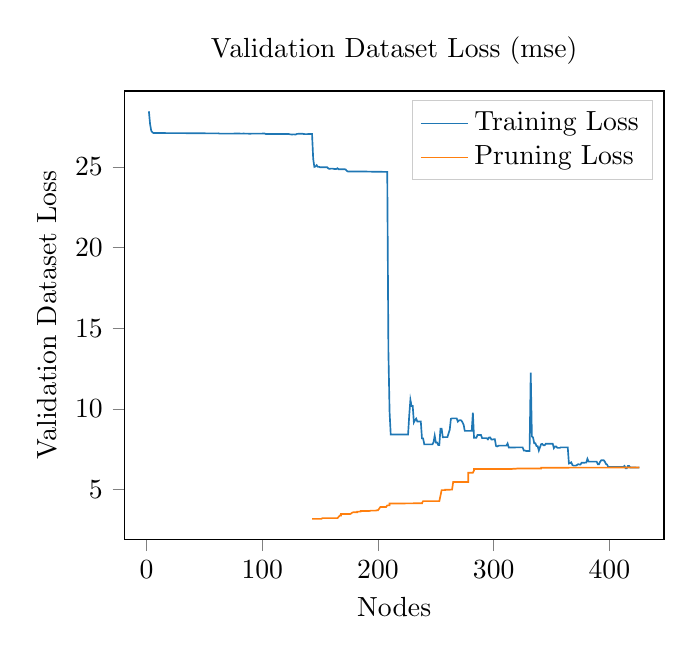
\begin{tikzpicture}

\definecolor{color0}{rgb}{0.12156862745098,0.466666666666667,0.705882352941177}
\definecolor{color1}{rgb}{1,0.498039215686275,0.0549019607843137}

\begin{axis}[
title={Validation Dataset Loss (mse)},
xlabel={Nodes},
ylabel={Validation Dataset Loss},
xmin=-19.2, xmax=447.2,
ymin=1.9267052, ymax=29.7153334666667,
tick align=outside,
tick pos=left,
x grid style={white!69.01960784313725!black},
y grid style={white!69.01960784313725!black},
legend cell align={left},
legend style={draw=white!80.0!black},
legend entries={{Training Loss},{Pruning Loss}}
]
\addlegendimage{no markers, color0}
\addlegendimage{no markers, color1}
\addplot [semithick, color0]
table {%
2 28.452214
3 27.6652506666667
4 27.2539146666667
5 27.1535066666667
6 27.107
7 27.107
8 27.1052826666667
9 27.1052826666667
10 27.1052826666667
11 27.1052826666667
12 27.1052826666667
13 27.1052826666667
14 27.1052826666667
15 27.1052826666667
16 27.1052826666667
17 27.101166
18 27.101166
19 27.101166
20 27.101166
21 27.101166
22 27.101166
23 27.101166
24 27.101166
25 27.101166
26 27.101166
27 27.1010186666667
28 27.1010186666667
29 27.1010186666667
30 27.101022
31 27.1014813333333
32 27.10203
33 27.10175
34 27.0981926666667
35 27.0981926666667
36 27.0981926666667
37 27.0981926666667
38 27.0981926666667
39 27.0981926666667
40 27.0944406666667
41 27.0920833333333
42 27.0912726666667
43 27.090532
44 27.0901766666667
45 27.0901766666667
46 27.0901766666667
47 27.090532
48 27.090532
49 27.090532
50 27.0910086666667
51 27.0878513333333
52 27.0863626666667
53 27.086582
54 27.086596
55 27.086596
56 27.086596
57 27.086596
58 27.086612
59 27.086612
60 27.086612
61 27.086612
62 27.088436
63 27.0698493333333
64 27.0690093333333
65 27.0690093333333
66 27.0690093333333
67 27.0690093333333
68 27.0687293333333
69 27.0687293333333
70 27.0687293333333
71 27.0694713333333
72 27.0694713333333
73 27.0694713333333
74 27.0694713333333
75 27.0694713333333
76 27.075696
77 27.0733426666667
78 27.0733426666667
79 27.0733426666667
80 27.074136
81 27.0724
82 27.0724
83 27.070576
84 27.0768246666667
85 27.0694646666667
86 27.06764
87 27.0677626666667
88 27.0671893333333
89 27.0671893333333
90 27.0665813333333
91 27.0693433333333
92 27.0693433333333
93 27.0693433333333
94 27.06929
95 27.06929
96 27.06929
97 27.06929
98 27.06929
99 27.06929
100 27.073066
101 27.074074
102 27.075988
103 27.046374
104 27.043878
105 27.0424273333333
106 27.043028
107 27.043028
108 27.043028
109 27.043028
110 27.043028
111 27.043028
112 27.043028
113 27.043028
114 27.043028
115 27.043028
116 27.0434973333333
117 27.0434973333333
118 27.043014
119 27.043014
120 27.043508
121 27.043508
122 27.043508
123 27.043508
124 27.02691
125 27.017764
126 27.0176553333333
127 27.0229933333333
128 27.0199046666667
129 27.0199046666667
130 27.0571973333333
131 27.0571313333333
132 27.0594006666667
133 27.0594006666667
134 27.0594006666667
135 27.0594426666667
136 27.0430426666667
137 27.0404053333333
138 27.0405013333333
139 27.0405013333333
140 27.0482106666667
141 27.0432826666667
142 27.0443813333333
143 27.0443813333333
144 25.4983333333333
145 25.0077026666667
146 25.0344893333333
147 25.1165906666667
148 25.0093086666667
149 25.010314
150 24.9848526666667
151 24.9860893333333
152 24.9860893333333
153 24.9860893333333
154 24.9860893333333
155 24.9860893333333
156 24.9860893333333
157 24.916516
158 24.883164
159 24.8986226666667
160 24.8986226666667
161 24.8986226666667
162 24.881244
163 24.8810413333333
164 24.8809033333333
165 24.925394
166 24.8606873333333
167 24.8605833333333
168 24.8605833333333
169 24.8568233333333
170 24.8614873333333
171 24.8631833333333
172 24.8515733333333
173 24.7642193333333
174 24.723878
175 24.723988
176 24.7237106666667
177 24.7237826666667
178 24.7237826666667
179 24.7238466666667
180 24.7238466666667
181 24.7238466666667
182 24.7238466666667
183 24.724084
184 24.724084
185 24.719196
186 24.7244626666667
187 24.7207233333333
188 24.7207233333333
189 24.7207233333333
190 24.7207793333333
191 24.7138913333333
192 24.7138913333333
193 24.7138913333333
194 24.7144326666667
195 24.7063746666667
196 24.7063746666667
197 24.70602
198 24.70602
199 24.70602
200 24.70602
201 24.70602
202 24.70602
203 24.70602
204 24.7003846666667
205 24.7003846666667
206 24.7003846666667
207 24.7003846666667
208 24.7003846666667
209 13.5285906666667
210 9.82925733333334
211 8.42235333333334
212 8.42227333333334
213 8.42227333333334
214 8.42227333333334
215 8.42218266666667
216 8.42218266666667
217 8.42218266666667
218 8.42218266666667
219 8.42218266666667
220 8.42166333333334
221 8.42166333333334
222 8.42166333333334
223 8.42166333333334
224 8.42158
225 8.42158
226 8.42158
227 9.61238
228 10.572944
229 10.19183
230 10.19183
231 9.172546
232 9.30909
233 9.40623
234 9.226036
235 9.226036
236 9.226036
237 9.226036
238 8.18194533333334
239 8.17536733333334
240 7.80672733333333
241 7.80807733333334
242 7.80807733333334
243 7.80672733333333
244 7.80672733333333
245 7.80672733333333
246 7.80672733333333
247 7.80672733333333
248 7.94948133333333
249 8.34970866666667
250 7.92976933333334
251 7.92976933333334
252 7.77383666666667
253 7.77335666666667
254 8.78666866666666
255 8.78666866666666
256 8.253122
257 8.25572533333333
258 8.25572533333333
259 8.25572533333333
260 8.25572533333333
261 8.491672
262 8.712056
263 9.39554733333333
264 9.42094666666667
265 9.42094666666667
266 9.42094666666667
267 9.42094666666667
268 9.42094666666667
269 9.21922866666666
270 9.29606866666666
271 9.30583666666667
272 9.29361866666667
273 9.17881866666667
274 9.03065666666667
275 8.64477866666667
276 8.64477866666667
277 8.64477866666667
278 8.64477866666667
279 8.64477866666667
280 8.64477866666667
281 8.64477866666667
282 9.77413066666667
283 8.21282933333333
284 8.21511866666667
285 8.21511866666667
286 8.39020666666667
287 8.39020666666667
288 8.39020666666667
289 8.39020666666667
290 8.19704866666667
291 8.19704866666667
292 8.19704866666667
293 8.19704866666667
294 8.19704866666667
295 8.12401866666667
296 8.23638133333334
297 8.23638133333334
298 8.10891466666667
299 8.10891466666667
300 8.12583133333334
301 8.12583133333334
302 7.710652
303 7.67876733333334
304 7.721154
305 7.73238066666667
306 7.73238066666667
307 7.73238066666667
308 7.73238066666667
309 7.731258
310 7.731258
311 7.73106
312 7.865612
313 7.61987866666667
314 7.61987866666667
315 7.62007666666667
316 7.62007666666667
317 7.62007666666667
318 7.62007666666667
319 7.62007666666667
320 7.62228466666667
321 7.62228466666667
322 7.62228466666667
323 7.62228466666667
324 7.62228466666667
325 7.62228466666667
326 7.43023266666667
327 7.426844
328 7.40296733333334
329 7.40296733333334
330 7.40296733333334
331 7.40296733333334
332 12.2624073333333
333 8.297714
334 8.241306
335 7.88352
336 7.88352
337 7.69828333333334
338 7.69828333333334
339 7.42608933333334
340 7.62848933333334
341 7.82235066666667
342 7.83763866666667
343 7.74933533333333
344 7.74933533333333
345 7.85473266666667
346 7.850976
347 7.850976
348 7.851072
349 7.851072
350 7.85115466666667
351 7.85115466666667
352 7.57315466666667
353 7.677248
354 7.680422
355 7.59454466666667
356 7.59454466666667
357 7.59454466666667
358 7.62047266666667
359 7.62047266666667
360 7.62047266666667
361 7.62047266666667
362 7.62047266666667
363 7.62047266666667
364 7.62047266666667
365 6.622618
366 6.64690733333333
367 6.69807733333333
368 6.53115066666667
369 6.49190266666667
370 6.49190266666667
371 6.49190266666667
372 6.52773666666667
373 6.58006266666667
374 6.56615066666667
375 6.56615066666667
376 6.66788866666667
377 6.66788866666667
378 6.66788866666667
379 6.67892866666667
380 6.67892866666667
381 6.91505333333334
382 6.73913
383 6.73913
384 6.73913
385 6.73913
386 6.73913
387 6.73913
388 6.73913
389 6.73913
390 6.57410666666667
391 6.57410666666667
392 6.73679666666667
393 6.82721333333333
394 6.82721333333333
395 6.82721333333333
396 6.74914933333333
397 6.59437266666667
398 6.558036
399 6.41215066666667
400 6.41215066666667
401 6.41215066666667
402 6.41215066666667
403 6.41215066666667
404 6.41215066666667
405 6.41215066666667
406 6.41303933333333
407 6.41303933333333
408 6.41303933333333
409 6.41303933333333
410 6.41303933333333
411 6.41150333333333
412 6.40927733333333
413 6.47082733333333
414 6.32734666666667
415 6.32734666666667
416 6.47489666666667
417 6.47489666666667
418 6.37368133333333
419 6.374668
420 6.374668
421 6.374668
422 6.374668
423 6.370508
424 6.370508
425 6.370508
426 6.37062
};
\addplot [semithick, color1]
table {%
426 6.37062
426 6.37062
425 6.37062
423 6.37062
423 6.37062
422 6.37062
422 6.37062
421 6.37062
419 6.37062
418 6.37062
418 6.37062
418 6.37062
418 6.37062
416 6.37062
414 6.37062
414 6.37062
413 6.37062
413 6.37062
412 6.37062
412 6.37061666666667
410 6.37061666666667
409 6.37061666666667
408 6.37061666666667
408 6.37061666666667
408 6.37061666666667
406 6.37061666666667
406 6.37061666666667
404 6.37061666666667
403 6.37061666666667
403 6.37061666666667
403 6.37061666666667
403 6.37061666666667
403 6.37061666666667
403 6.37061666666667
403 6.37061666666667
402 6.37061666666667
402 6.37061666666667
401 6.37061666666667
401 6.37014
399 6.36978466666667
397 6.36978466666667
397 6.36978466666667
397 6.36977066666667
396 6.36955133333333
396 6.36955133333333
395 6.36955133333333
394 6.36955133333333
392 6.36955133333333
392 6.36955133333333
391 6.36955133333333
391 6.36955133333333
389 6.36953533333333
388 6.36953533333333
388 6.36953533333333
388 6.36953533333333
388 6.36953533333333
388 6.36953533333333
387 6.36953533333333
387 6.36953533333333
387 6.36879333333333
387 6.36879333333333
385 6.36879333333333
383 6.36879333333333
383 6.36879333333333
382 6.36879333333333
381 6.36879333333333
380 6.36879333333333
379 6.36879333333333
379 6.36879333333333
378 6.36879333333333
378 6.36879333333333
378 6.36879333333333
377 6.36879333333333
376 6.36879333333333
376 6.36879333333333
376 6.36768866666667
371 6.36768866666667
371 6.367566
371 6.367566
370 6.367566
369 6.367566
369 6.367566
369 6.367566
369 6.367566
369 6.367566
368 6.367566
367 6.367566
367 6.367566
367 6.367566
365 6.367566
365 6.366558
365 6.364644
363 6.360868
361 6.360868
360 6.35815933333333
357 6.35815933333333
357 6.35815933333333
357 6.35815933333333
356 6.35815933333333
356 6.35815933333333
354 6.35755866666667
354 6.35755866666667
354 6.35755866666667
352 6.35755866666667
352 6.35755866666667
350 6.35755866666667
350 6.35755866666667
350 6.35755866666667
349 6.35755866666667
348 6.35755866666667
347 6.35755866666667
346 6.35755866666667
346 6.35755866666667
346 6.35755866666667
344 6.35755866666667
343 6.35706466666667
342 6.35706466666667
342 6.35706466666667
341 6.35706466666667
341 6.35481533333333
341 6.31752266666667
338 6.31752266666667
338 6.31752266666667
338 6.31752266666667
336 6.31525333333333
336 6.31521133333333
334 6.31521133333333
334 6.31521133333333
334 6.31511533333333
334 6.31511533333333
332 6.31511533333333
332 6.31401666666667
332 6.31401666666667
330 6.31401666666667
330 6.31123533333334
328 6.31123533333334
328 6.31123533333334
328 6.31023
327 6.31023
327 6.31023
326 6.31023
325 6.30899333333333
325 6.30899333333333
324 6.30899333333333
323 6.30899333333333
321 6.30899333333333
321 6.30899333333333
321 6.30899333333333
320 6.30899333333333
319 6.29353466666667
319 6.29353466666667
318 6.29353466666667
318 6.29353466666667
318 6.29353466666667
318 6.29353466666667
318 6.29353466666667
318 6.29353466666667
317 6.29353466666667
317 6.29353466666667
317 6.29183866666667
316 6.28717466666667
316 6.28717466666667
315 6.28717466666667
315 6.28717466666667
315 6.28706466666667
315 6.28706466666667
315 6.28706466666667
314 6.28706466666667
314 6.28706466666667
312 6.28700066666667
310 6.28692866666667
310 6.28692866666667
309 6.28669133333333
307 6.28669133333333
306 6.28669133333333
306 6.28669133333333
305 6.28669133333333
305 6.28663533333333
303 6.28663533333333
303 6.28663533333333
302 6.28663533333333
302 6.286094
300 6.286094
300 6.286094
300 6.286094
299 6.286094
298 6.286094
298 6.286094
297 6.286094
296 6.286094
296 6.286094
295 6.286094
295 6.286094
294 6.286094
294 6.286094
293 6.286094
292 6.286094
292 6.286094
292 6.286094
292 6.286094
291 6.286094
291 6.286094
290 6.286094
290 6.286094
289 6.286094
289 6.286094
288 6.286094
287 6.286094
287 6.286094
286 6.286094
286 6.286094
285 6.286094
285 6.286094
284 6.286094
284 6.286094
283 6.286094
283 6.188954
282 6.05241
281 6.05241
281 6.05241
281 6.05241
280 6.05241
280 6.05241
278 6.05241
278 5.481638
273 5.481638
272 5.481638
272 5.481638
271 5.481638
271 5.481638
270 5.481638
269 5.481638
269 5.481638
268 5.481638
268 5.481638
268 5.481638
268 5.481638
265 5.481638
265 5.481638
265 5.481638
264 5.00187266666667
264 5.00187266666667
263 5.00187266666667
263 5.00187266666667
261 4.99926933333334
258 4.99926933333334
258 4.99926933333334
258 4.97387
258 4.97387
257 4.97387
257 4.97387
255 4.97387
253 4.29037866666667
253 4.29037866666667
253 4.29037866666667
253 4.29037866666667
253 4.29037866666667
253 4.29037866666667
252 4.29037866666667
252 4.29037866666667
251 4.29037866666667
251 4.29037866666667
251 4.29037866666667
249 4.29037866666667
249 4.29037866666667
247 4.29037866666667
246 4.29037866666667
246 4.29037866666667
246 4.29037866666667
246 4.29037866666667
244 4.29037866666667
244 4.29037866666667
243 4.29037866666667
242 4.29037866666667
242 4.29037866666667
242 4.29037866666667
240 4.29037866666667
239 4.29037866666667
239 4.29037866666667
238 4.178016
238 4.16109933333333
238 4.16109933333333
236 4.16109933333333
235 4.16109933333333
234 4.16109933333333
234 4.16109933333333
234 4.16109933333333
234 4.16109933333333
232 4.16109933333333
232 4.16109933333333
232 4.16109933333333
231 4.16109933333333
230 4.15119333333333
230 4.15119333333333
229 4.15119333333333
229 4.15119333333333
228 4.15119333333333
227 4.15099533333333
226 4.15099533333333
223 4.15099533333333
223 4.14878733333333
223 4.14878733333333
222 4.14878733333333
220 4.14878733333333
220 4.14878733333333
220 4.14878733333333
218 4.14878733333333
216 4.14878733333333
215 4.14878733333333
215 4.14878733333333
215 4.14878733333333
214 4.14878733333333
214 4.14878733333333
213 4.14878733333333
212 4.14878733333333
212 4.14878733333333
212 4.14878733333333
211 4.14878733333333
211 4.14878733333333
210 4.14878733333333
210 4.14878733333333
210 4.13349933333333
210 4.13349933333333
210 4.028102
208 4.028102
207 3.922544
207 3.922544
207 3.922544
207 3.922544
206 3.92246133333333
204 3.92236533333333
202 3.92236533333333
200 3.723722
200 3.723722
200 3.723722
200 3.723722
199 3.723722
198 3.702332
198 3.702332
198 3.702332
197 3.702332
195 3.702332
195 3.702332
194 3.702332
192 3.676404
188 3.676404
186 3.676404
186 3.676404
186 3.676404
185 3.676404
185 3.64057
183 3.64057
183 3.64057
182 3.64057
182 3.602156
180 3.602156
180 3.602156
179 3.602156
179 3.602156
178 3.591116
176 3.489378
175 3.489378
175 3.489378
174 3.489378
174 3.489378
173 3.489378
173 3.489378
172 3.489378
170 3.489378
168 3.489378
168 3.489378
168 3.39896133333333
168 3.39896133333333
167 3.39896133333333
165 3.23627133333333
163 3.23627133333333
163 3.23627133333333
163 3.23627133333333
163 3.23627133333333
162 3.23627133333333
162 3.23627133333333
161 3.23627133333333
161 3.23627133333333
160 3.23627133333333
158 3.23627133333333
157 3.23627133333333
157 3.23627133333333
156 3.23627133333333
156 3.23627133333333
154 3.23627133333333
154 3.23627133333333
153 3.23627133333333
153 3.23627133333333
153 3.23627133333333
152 3.23627133333333
152 3.23627133333333
152 3.23627133333333
151 3.18993666666667
149 3.18993666666667
149 3.18993666666667
149 3.18993666666667
147 3.18993666666667
147 3.18993666666667
146 3.18993666666667
146 3.18982466666667
144 3.18982466666667
143 3.18982466666667
143 3.18982466666667
143 3.18982466666667
143 3.18982466666667
};
\end{axis}

\end{tikzpicture}
% This file was created by matplotlib2tikz v0.6.17.
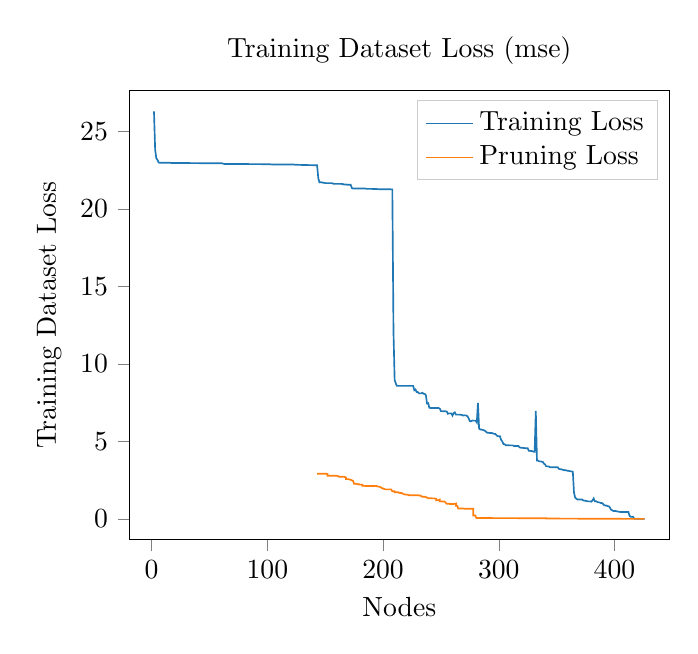
\begin{tikzpicture}

\definecolor{color0}{rgb}{0.12156862745098,0.466666666666667,0.705882352941177}
\definecolor{color1}{rgb}{1,0.498039215686275,0.0549019607843137}

\begin{axis}[
title={Training Dataset Loss (mse)},
xlabel={Nodes},
ylabel={Training Dataset Loss},
xmin=-19.2, xmax=447.2,
ymin=-1.3149935915493, ymax=27.6148654225352,
tick align=outside,
tick pos=left,
x grid style={white!69.01960784313725!black},
y grid style={white!69.01960784313725!black},
legend cell align={left},
legend style={draw=white!80.0!black},
legend entries={{Training Loss},{Pruning Loss}}
]
\addlegendimage{no markers, color0}
\addlegendimage{no markers, color1}
\addplot [semithick, color0]
table {%
2 26.2998718309859
3 23.8300622065728
4 23.2778143192488
5 23.1705100938967
6 22.9962377934272
7 22.9839842723005
8 22.9837213615024
9 22.9832246478873
10 22.9830406103286
11 22.9830396713615
12 22.9827230046948
13 22.9826551643193
14 22.9826316901409
15 22.982391314554
16 22.9823575117371
17 22.9634021126761
18 22.9629387323944
19 22.9620401408451
20 22.9620363849765
21 22.962032629108
22 22.9620323943662
23 22.9620208920188
24 22.962003286385
25 22.9619974178404
26 22.9616028169014
27 22.9614929577465
28 22.9614779342723
29 22.9614779342723
30 22.9614720657277
31 22.962084741784
32 22.960488028169
33 22.9600361502348
34 22.9592464788733
35 22.9592544600939
36 22.9592544600939
37 22.9589830985916
38 22.9583962441315
39 22.9583201877934
40 22.9572664319249
41 22.9537509389671
42 22.9535105633803
43 22.9534821596244
44 22.9523922535211
45 22.9522455399061
46 22.9522058685446
47 22.9512049295775
48 22.9511370892019
49 22.9510974178404
50 22.9510690140845
51 22.9475535211268
52 22.9471518779343
53 22.9471403755869
54 22.9470368544601
55 22.9465410798122
56 22.9463298122066
57 22.9462769953052
58 22.9462497652582
59 22.9462460093897
60 22.946185915493
61 22.9460147887324
62 22.913473943662
63 22.9032899061033
64 22.9026056338028
65 22.9025718309859
66 22.9025568075118
67 22.9026338028169
68 22.9025680751174
69 22.9025643192488
70 22.9025305164319
71 22.9024269953052
72 22.9023234741784
73 22.9018352112676
74 22.9017070422535
75 22.9016920187794
76 22.9009600938967
77 22.899482629108
78 22.8990169014085
79 22.8985201877934
80 22.8986539906103
81 22.8977516431925
82 22.8973570422535
83 22.8970180751174
84 22.8956723004695
85 22.8928741784038
86 22.8927392018779
87 22.8927382629108
88 22.8927147887324
89 22.8924744131455
90 22.8921354460094
91 22.8908328638498
92 22.8910647887324
93 22.8905894366197
94 22.8905884976526
95 22.8883340375587
96 22.887970657277
97 22.8882147887324
98 22.8873124413146
99 22.8868157276995
100 22.8866129107981
101 22.8865791079812
102 22.8865507042254
103 22.8780420187793
104 22.8705715962441
105 22.86735657277
106 22.8660626760563
107 22.8655873239437
108 22.865527230047
109 22.8655269953052
110 22.8655269953052
111 22.8652218309859
112 22.8650697183099
113 22.8650169014084
114 22.8647612676056
115 22.8647610328639
116 22.8646267605634
117 22.8645025821596
118 22.8643558685446
119 22.86435
120 22.8642427230047
121 22.8642877934272
122 22.8642417840376
123 22.8641478873239
124 22.8549321596244
125 22.8526335680751
126 22.8527124413146
127 22.8469262910798
128 22.8439288732394
129 22.8429063380282
130 22.8362018779343
131 22.8361934272301
132 22.836158685446
133 22.8354741784038
134 22.8342232394366
135 22.8342117370892
136 22.825934741784
137 22.8254183098592
138 22.8253422535211
139 22.8252575117371
140 22.8219889671362
141 22.8218443661972
142 22.821829342723
143 22.8214903755869
144 21.9846115023474
145 21.714946713615
146 21.7294603286385
147 21.7179936619718
148 21.69485
149 21.6946525821596
150 21.668841314554
151 21.6686319248826
152 21.6678605633803
153 21.6677469483568
154 21.6675213615024
155 21.6675204225352
156 21.6674265258216
157 21.6241636150235
158 21.6190819248826
159 21.6178690140845
160 21.617697887324
161 21.6176694835681
162 21.6154150234742
163 21.6153737089202
164 21.6153715962441
165 21.6131105633803
166 21.5775847417841
167 21.5775450704225
168 21.5775429577465
169 21.5647448356808
170 21.5643877934272
171 21.5617502347418
172 21.5613161971831
173 21.3522267605634
174 21.3220708920188
175 21.3220424882629
176 21.321741314554
177 21.3216309859155
178 21.3216225352113
179 21.3216
180 21.3215997652582
181 21.3215997652582
182 21.3215997652582
183 21.3215150234742
184 21.3215147887324
185 21.3132622065728
186 21.2966462441315
187 21.2942354460094
188 21.2942016431925
189 21.2941901408451
190 21.2941441314554
191 21.2915262910798
192 21.2914323943662
193 21.2914321596244
194 21.2913861502348
195 21.278432629108
196 21.2763622065728
197 21.2763161971831
198 21.2761866197183
199 21.2761582159625
200 21.2761579812207
201 21.2758009389672
202 21.2684403755869
203 21.2685492957747
204 21.2670842723005
205 21.2670758215963
206 21.2661734741784
207 21.2661274647888
208 21.2638730046949
209 12.056641314554
210 8.96405915492959
211 8.7346647887324
212 8.58417089201879
213 8.58397347417841
214 8.58394507042254
215 8.58402769953052
216 8.5837647887324
217 8.58376384976527
218 8.58376009389672
219 8.58367558685447
220 8.5832809859155
221 8.5832809859155
222 8.58288638497653
223 8.58282159624414
224 8.58267488262912
225 8.58208802816902
226 8.58202018779344
227 8.29904929577466
228 8.35155446009391
229 8.1871016431925
230 8.18574577464789
231 8.10072206572771
232 8.09711455399062
233 8.09663920187794
234 8.13432746478874
235 8.067870657277
236 8.06732981220658
237 7.97854460093897
238 7.44682629107982
239 7.46758051643193
240 7.1695147887324
241 7.15844577464789
242 7.15681056338029
243 7.15549014084507
244 7.15548920187794
245 7.15515023474179
246 7.15403262910799
247 7.15394788732395
248 7.15484835680752
249 7.11849460093897
250 6.9524661971831
251 6.95207159624414
252 6.9467192488263
253 6.95209014084507
254 6.93929014084507
255 6.93708145539907
256 6.77924107981221
257 6.80979530516432
258 6.80744553990611
259 6.80714131455399
260 6.66395798122066
261 6.83158990610329
262 6.87567253521127
263 6.73037934272301
264 6.73015375586855
265 6.72784389671362
266 6.72615375586855
267 6.7159
268 6.71428286384977
269 6.66600093896714
270 6.68467699530517
271 6.67770516431925
272 6.67415375586855
273 6.61733122065728
274 6.48294553990611
275 6.30074812206573
276 6.30062394366198
277 6.34612816901409
278 6.34117042253521
279 6.34005281690141
280 6.33564694835681
281 6.22421009389672
282 7.48896877934272
283 5.8203265258216
284 5.76873591549296
285 5.76596502347418
286 5.74308615023474
287 5.71825516431925
288 5.68611901408451
289 5.62042863849765
290 5.55913262910798
291 5.55747629107981
292 5.54709131455399
293 5.54312417840376
294 5.54304812206573
295 5.51641220657277
296 5.48462253521127
297 5.48401197183099
298 5.39604201877934
299 5.34060539906103
300 5.33693755868545
301 5.33637394366197
302 5.09966713615023
303 5.00433732394366
304 4.83215704225352
305 4.82401338028169
306 4.74917394366197
307 4.74824225352113
308 4.74817441314554
309 4.74831056338028
310 4.74323802816901
311 4.74320962441315
312 4.74200234741784
313 4.70810563380282
314 4.69963145539906
315 4.69910915492958
316 4.6990161971831
317 4.69900469483568
318 4.61583098591549
319 4.58751643192488
320 4.58738122065728
321 4.57722535211268
322 4.57506197183099
323 4.55811549295775
324 4.55806948356808
325 4.55806572769953
326 4.38909953051643
327 4.38724788732394
328 4.38231244131455
329 4.37146150234742
330 4.33704647887324
331 4.32960892018779
332 6.9706089201878
333 3.76501267605634
334 3.75413661971831
335 3.7133176056338
336 3.7133176056338
337 3.69148075117371
338 3.69082136150235
339 3.56175962441315
340 3.51822159624413
341 3.38965633802817
342 3.38958028169014
343 3.3910558685446
344 3.34224460093897
345 3.33593098591549
346 3.33343497652582
347 3.33341995305164
348 3.33349600938967
349 3.33332488262911
350 3.33332394366197
351 3.33317723004695
352 3.2247265258216
353 3.20666079812207
354 3.20664178403756
355 3.17130281690141
356 3.15542488262911
357 3.13943403755869
358 3.14277136150235
359 3.11012558685446
360 3.10965023474178
361 3.08203309859155
362 3.0792441314554
363 3.05146572769953
364 3.05130704225352
365 1.69420704225352
366 1.37397558685446
367 1.30442276995305
368 1.25575610328639
369 1.25519835680751
370 1.25481384976526
371 1.25323544600939
372 1.24968403755869
373 1.18790727699531
374 1.1763382629108
375 1.1706985915493
376 1.14462605633803
377 1.13120117370892
378 1.12962276995305
379 1.12952887323944
380 1.11019342723005
381 1.19776596244131
382 1.31716384976526
383 1.13703708920188
384 1.13693356807512
385 1.09767511737089
386 1.06708333333333
387 1.0631161971831
388 1.029929342723
389 1.0242896713615
390 0.978475821596244
391 0.886779812206573
392 0.869182394366197
393 0.863542723004695
394 0.821540610328638
395 0.820638262910798
396 0.736811502347418
397 0.599352582159625
398 0.559600234741784
399 0.511216197183099
400 0.510506103286385
401 0.509229107981221
402 0.485341549295775
403 0.475185680751174
404 0.450238262910798
405 0.449021361502348
406 0.448516666666667
407 0.44851220657277
408 0.448507511737089
409 0.448488497652582
410 0.448412441314554
411 0.448336384976526
412 0.446753990610329
413 0.209584741784038
414 0.131432394366197
415 0.13116103286385
416 0.136915962441315
417 0.0222208920187794
418 0.00288544600938968
419 0.00335023474178406
420 0.00381502347417843
421 0.00358943661971833
422 0.00253568075117372
423 0.000118779342723001
424 0.000109859154929576
425 3.3802816901407e-05
426 0
};
\addplot [semithick, color1]
table {%
426 0.000496713615023472
426 0.000497652582159623
425 0.000681690140845068
423 0.000681690140845068
423 0.000705164319248823
422 0.000773004694835678
422 0.000806807511737086
421 0.00104718309859155
419 0.00136384976525821
418 0.00136384976525821
418 0.00136760563380281
418 0.00136784037558685
418 0.00137934272300469
416 0.00138309859154929
414 0.00228169014084507
414 0.00267629107981221
413 0.00268215962441315
413 0.00268215962441315
412 0.00269718309859155
412 0.00270305164319249
410 0.00270305164319249
409 0.00270305164319249
408 0.00270305164319249
408 0.00297441314553991
408 0.00356126760563381
406 0.00356126760563381
406 0.00363732394366197
404 0.0036293427230047
403 0.0036293427230047
403 0.0036293427230047
403 0.0036293427230047
403 0.0036293427230047
403 0.0036293427230047
403 0.0036293427230047
403 0.00366901408450704
402 0.00381572769953052
402 0.00385539906103286
401 0.00392323943661972
401 0.00395164319248826
399 0.00495258215962442
397 0.00495258215962442
397 0.00495258215962442
397 0.00505610328638498
396 0.00506760563380282
396 0.00512042253521127
395 0.00533169014084508
394 0.0058274647887324
392 0.0058274647887324
392 0.00588755868544601
391 0.00589131455399061
391 0.00606244131455399
389 0.00608967136150235
388 0.00608967136150235
388 0.00608967136150235
388 0.00608967136150235
388 0.00608967136150235
388 0.00610469483568075
387 0.00613849765258216
387 0.00614225352112676
387 0.00624577464788732
387 0.00634929577464789
385 0.0063830985915493
383 0.0063830985915493
383 0.0063981220657277
382 0.00652629107981221
381 0.00701455399061033
380 0.00701455399061033
379 0.00701455399061033
379 0.0075112676056338
378 0.00797699530516432
378 0.00797699530516432
378 0.00837159624413146
377 0.00837159624413146
376 0.00837159624413146
376 0.00837159624413146
376 0.0116884976525822
371 0.0116884976525822
371 0.0116894366197183
371 0.0119298122065728
370 0.0119298122065728
369 0.0119298122065728
369 0.0119298122065728
369 0.0119298122065728
369 0.0124051643192488
369 0.0146596244131455
368 0.0146596244131455
367 0.0146596244131455
367 0.0155619718309859
367 0.0160586854460094
365 0.0158145539906103
365 0.0158483568075117
365 0.0158767605633803
363 0.0160795774647887
361 0.0164429577464789
360 0.0175145539906103
357 0.0175145539906103
357 0.0175145539906103
357 0.0175746478873239
356 0.01805
356 0.018050234741784
354 0.019344131455399
354 0.0193969483568075
354 0.0196525821596244
352 0.0198046948356807
352 0.0198049295774648
350 0.0201100938967136
350 0.0202342723004695
350 0.0202401408450704
349 0.0202401408450704
348 0.0202401408450704
347 0.0202401408450704
346 0.0202401408450704
346 0.0202861502347418
346 0.0203800469483568
344 0.0203349765258216
343 0.0204422535211267
342 0.0204422535211267
342 0.0214647887323943
341 0.0214647887323943
341 0.0302483568075117
341 0.0369528169014084
338 0.0369528169014084
338 0.0376373239436619
338 0.0388882629107981
336 0.0389230046948357
336 0.0389345070422535
334 0.0389345070422535
334 0.0389345070422535
334 0.0390105633802817
334 0.0390953051643192
332 0.0390953051643192
332 0.0391103286384976
332 0.0394492957746478
330 0.0394492957746478
330 0.0428624413145539
328 0.0428624413145539
328 0.0428624413145539
328 0.0430598591549295
327 0.0430598591549295
327 0.0431734741784037
326 0.0439448356807511
325 0.0441542253521126
325 0.0442481220657277
324 0.0442490610328638
323 0.0444746478873239
321 0.0444746478873239
321 0.0444746478873239
321 0.0445030516431925
320 0.0446741784037558
319 0.0458870892018779
319 0.0458870892018779
318 0.0458870892018779
318 0.0458870892018779
318 0.0458870892018779
318 0.0458870892018779
318 0.0458870892018779
318 0.0458892018779342
317 0.0458892018779342
317 0.0458892018779342
317 0.0485267605633802
316 0.0488838028169014
316 0.0488838028169014
315 0.0488838028169014
315 0.0488838028169014
315 0.0489122065727699
315 0.0489206572769953
315 0.0489206572769953
314 0.0489208920187793
314 0.0489208920187793
312 0.0489434272300469
310 0.0490537558685446
310 0.0490539906103286
309 0.0491387323943661
307 0.0491387323943661
306 0.0491387323943661
306 0.049150234741784
305 0.0491840375586854
305 0.0492300469483568
303 0.0492300469483568
303 0.0492302816901408
302 0.0493241784037558
302 0.0493701877934272
300 0.0493701877934272
300 0.0493701877934272
300 0.0493985915492957
299 0.0495281690140844
298 0.0495281690140844
298 0.0498852112676056
297 0.0498854460093896
296 0.0498854460093896
296 0.049893896713615
295 0.049893896713615
295 0.0507962441314553
294 0.0507962441314553
294 0.0530507042253521
293 0.0530967136150234
292 0.0530967136150234
292 0.0530967136150234
292 0.0530967136150234
292 0.053125117370892
291 0.0533225352112676
291 0.0533262910798122
290 0.0533272300469483
290 0.0533272300469483
289 0.0533272300469483
289 0.0537218309859155
288 0.0537218309859155
287 0.0537218309859155
287 0.0543086854460093
286 0.0543086854460093
286 0.0543765258215962
285 0.0543765258215962
285 0.0543765258215962
284 0.0543765258215962
284 0.0557323943661972
283 0.0557323943661972
283 0.0562077464788732
282 0.0598152582159624
281 0.0598152582159624
281 0.0598152582159624
281 0.060356103286385
280 0.126812910798122
280 0.215598122065728
278 0.215598122065728
278 0.657852112676057
273 0.657853051643193
272 0.657853051643193
272 0.658192018779343
271 0.658192018779343
271 0.658276760563381
270 0.659394366197184
269 0.673419014084507
269 0.673813615023475
268 0.673813615023475
268 0.673813615023475
268 0.673813615023475
268 0.673813615023475
265 0.673813615023475
265 0.676022300469484
265 0.676022300469484
264 0.846662676056338
264 0.846966901408451
263 0.849316666666667
263 0.9925
261 0.961945774647888
258 0.961945774647888
258 0.961945774647888
258 0.962171361502348
258 0.972425117370892
257 0.974115258215963
257 0.975732394366198
255 0.978042253521127
253 1.12333544600939
253 1.12333544600939
253 1.12333544600939
253 1.12333544600939
253 1.12333544600939
253 1.12333544600939
252 1.12333544600939
252 1.12345962441315
251 1.12345962441315
251 1.12457723004695
251 1.12898309859155
249 1.13394084507042
249 1.24537769953052
247 1.1998734741784
246 1.1998734741784
246 1.1998734741784
246 1.23200962441315
246 1.2977
244 1.32253098591549
244 1.32418732394366
243 1.32418732394366
242 1.32418732394366
242 1.3281544600939
242 1.32823051643193
240 1.33861549295775
239 1.33861549295775
239 1.33922605633803
238 1.37101572769953
238 1.37468356807512
238 1.37524718309859
236 1.4306838028169
235 1.4306838028169
234 1.4306838028169
234 1.4306838028169
234 1.43161549295775
234 1.43168333333333
232 1.50652276995305
232 1.51159530516432
232 1.51159530516432
231 1.51159530516432
230 1.51963122065728
230 1.52810539906103
229 1.52810539906103
229 1.52811690140845
228 1.52820985915493
227 1.52873215962441
226 1.52873215962441
223 1.52873215962441
223 1.52886737089202
223 1.53103075117371
222 1.54118661971831
220 1.56950117370892
220 1.56954718309859
220 1.56955093896714
218 1.58649741784038
216 1.66967112676056
215 1.66967112676056
215 1.66967112676056
215 1.6805220657277
214 1.6805220657277
214 1.68795962441315
213 1.72237464788732
212 1.72237464788732
212 1.72237464788732
212 1.72237464788732
211 1.72237464788732
211 1.72303403755869
210 1.72303403755869
210 1.72303403755869
210 1.72311009389671
210 1.77192136150235
210 1.77823497652582
208 1.77823497652582
207 1.90532464788733
207 1.9053396713615
207 1.90551079812207
207 1.90565751173709
206 1.90565845070423
204 1.9055823943662
202 1.9055823943662
200 1.95161643192488
200 1.95161643192488
200 1.95161643192488
200 1.96760727699531
199 1.98348521126761
198 2.03690892018779
198 2.03738427230047
198 2.04017323943662
197 2.06779037558686
195 2.10043615023474
195 2.10059483568075
194 2.12837323943662
192 2.12503591549296
188 2.12503591549296
186 2.12503591549296
186 2.12503591549296
186 2.12661431924883
185 2.12699882629108
185 2.13055023474179
183 2.13055023474179
183 2.13618990610329
182 2.13618990610329
182 2.20953568075118
180 2.20953568075118
180 2.21111408450704
179 2.22453896713615
179 2.24387441314554
178 2.24396830985916
176 2.27004084507042
175 2.27004084507042
175 2.27014436619718
174 2.45027112676057
174 2.4542382629108
173 2.48483004694836
173 2.49046971830986
172 2.52365657276995
170 2.56291502347418
168 2.56291502347418
168 2.65461103286385
168 2.66025070422535
168 2.66115305164319
167 2.70315516431925
165 2.72075258215963
163 2.72075258215963
163 2.72075258215963
163 2.72075258215963
163 2.72146267605634
162 2.72146267605634
162 2.73161854460094
161 2.75550610328639
161 2.75672300469484
160 2.78167042253521
158 2.78294741784038
157 2.78294741784038
157 2.78296643192488
156 2.78297112676057
156 2.78304718309859
154 2.78305164319249
154 2.78305164319249
153 2.78305164319249
153 2.78305164319249
153 2.78332300469484
152 2.78332300469484
152 2.89801807511737
152 2.89801807511737
151 2.9115985915493
149 2.9115985915493
149 2.91182417840376
149 2.9128779342723
147 2.91241314553991
147 2.91248920187794
146 2.91249812206573
146 2.91253192488263
144 2.91253192488263
143 2.91253192488263
143 2.91253192488263
143 2.91253192488263
143 2.91253192488263
};
\end{axis}

\end{tikzpicture}

\subsection{Dataset 2}
A minimum mean squared validation loss of approx. \textbf{0.57} and absolute loss of \textbf{0.39} were observed after training. Very minor loss on training data was observed before pruning due to multiple samples having same features but different output values. The final tree had approx. \textbf{140-180 nodes} after pruning. As with dataset 1, each node leaf was constrained to 2 samples. For this dataset, a loss function with the probabilities of each split multiplying the loss yielded better results and much better timings.

% This file was created by matplotlib2tikz v0.6.17.
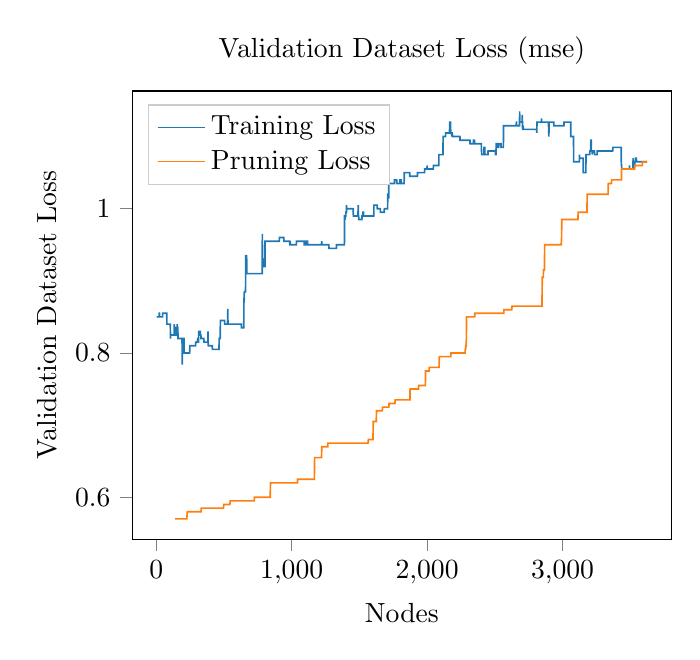
\begin{tikzpicture}

\definecolor{color0}{rgb}{0.12156862745098,0.466666666666667,0.705882352941177}
\definecolor{color1}{rgb}{1,0.498039215686275,0.0549019607843137}

\begin{axis}[
title={Validation Dataset Loss (mse)},
xlabel={Nodes},
ylabel={Validation Dataset Loss},
xmin=-179.15, xmax=3806.15,
ymin=0.54175, ymax=1.16325,
tick align=outside,
tick pos=left,
x grid style={white!69.01960784313725!black},
y grid style={white!69.01960784313725!black},
legend cell align={left},
legend style={at={(0.03,0.97)}, anchor=north west, draw=white!80.0!black},
legend entries={{Training Loss},{Pruning Loss}}
]
\addlegendimage{no markers, color0}
\addlegendimage{no markers, color1}
\addplot [semithick, color0]
table {%
2 0.85
3 0.85
4 0.85
5 0.85
6 0.85
7 0.85
8 0.85
9 0.85
10 0.85
11 0.85
12 0.85
13 0.85
14 0.85
15 0.85
16 0.85
17 0.85
18 0.85
19 0.85
20 0.85
21 0.85
22 0.855
23 0.855
25 0.85
26 0.85
27 0.85
28 0.85
29 0.85
30 0.85
31 0.85
32 0.85
33 0.85
34 0.85
35 0.85
36 0.85
37 0.85
38 0.85
39 0.85
40 0.85
41 0.85
42 0.85
43 0.85
44 0.85
45 0.85
46 0.85
47 0.855
48 0.855
50 0.855
51 0.855
52 0.855
53 0.855
54 0.855
55 0.855
56 0.855
57 0.855
58 0.855
59 0.855
60 0.855
61 0.855
62 0.855
63 0.855
64 0.855
66 0.855
67 0.855
68 0.855
69 0.855
70 0.855
71 0.855
72 0.855
73 0.855
74 0.855
75 0.855
76 0.855
77 0.855
78 0.84
79 0.84
80 0.84
81 0.84
82 0.84
83 0.84
84 0.84
85 0.84
86 0.84
87 0.84
88 0.84
89 0.84
90 0.84
91 0.84
92 0.84
93 0.84
94 0.84
95 0.84
96 0.84
97 0.84
98 0.84
99 0.84
100 0.84
102 0.84
103 0.84
105 0.82
106 0.825
107 0.825
108 0.825
109 0.825
110 0.825
111 0.825
112 0.825
113 0.825
114 0.825
115 0.825
116 0.825
117 0.825
118 0.825
119 0.825
122 0.825
123 0.825
125 0.825
126 0.825
127 0.825
130 0.825
131 0.825
133 0.84
134 0.835
135 0.835
136 0.835
137 0.835
138 0.835
139 0.835
140 0.835
141 0.83
142 0.83
143 0.825
144 0.825
145 0.825
146 0.825
147 0.825
150 0.825
151 0.825
152 0.825
153 0.825
154 0.825
155 0.84
156 0.835
157 0.835
159 0.835
160 0.82
161 0.82
162 0.82
163 0.82
164 0.82
165 0.82
166 0.82
167 0.82
169 0.82
170 0.82
171 0.82
173 0.82
174 0.82
175 0.82
176 0.82
178 0.82
179 0.82
180 0.82
181 0.82
182 0.82
183 0.82
184 0.82
185 0.82
186 0.82
187 0.82
188 0.82
189 0.82
190 0.82
191 0.785
192 0.785
193 0.82
194 0.82
195 0.82
197 0.82
198 0.82
199 0.82
200 0.82
201 0.82
202 0.82
203 0.82
204 0.82
205 0.8
206 0.8
207 0.8
209 0.8
210 0.8
211 0.8
212 0.8
213 0.8
214 0.8
215 0.8
216 0.8
217 0.8
218 0.8
219 0.8
220 0.8
221 0.8
222 0.8
223 0.8
224 0.8
227 0.8
228 0.8
229 0.8
230 0.8
231 0.8
232 0.8
233 0.8
234 0.8
235 0.8
237 0.8
238 0.8
239 0.8
240 0.8
241 0.8
243 0.8
244 0.8
245 0.8
246 0.8
247 0.805
248 0.81
249 0.81
250 0.81
251 0.81
253 0.81
254 0.81
255 0.81
256 0.81
257 0.81
258 0.81
260 0.81
261 0.81
263 0.81
264 0.81
265 0.81
266 0.81
268 0.81
269 0.81
270 0.81
271 0.81
272 0.81
273 0.81
274 0.81
275 0.81
276 0.81
277 0.81
278 0.81
279 0.81
280 0.81
281 0.81
282 0.81
283 0.81
284 0.81
285 0.81
286 0.81
287 0.81
288 0.81
290 0.81
291 0.815
292 0.815
293 0.815
294 0.815
295 0.815
296 0.815
297 0.815
298 0.815
299 0.815
300 0.815
301 0.815
303 0.815
304 0.815
305 0.82
306 0.82
307 0.82
308 0.82
309 0.815
310 0.815
311 0.815
312 0.815
313 0.83
314 0.83
315 0.83
317 0.83
318 0.83
319 0.83
320 0.83
321 0.83
322 0.83
323 0.83
324 0.83
325 0.825
326 0.825
327 0.825
328 0.825
329 0.825
330 0.82
331 0.82
332 0.82
333 0.82
334 0.82
335 0.82
336 0.82
337 0.82
338 0.82
339 0.82
340 0.82
341 0.82
342 0.82
343 0.82
344 0.82
345 0.82
346 0.82
348 0.82
350 0.82
351 0.82
352 0.815
353 0.815
354 0.815
355 0.815
356 0.815
357 0.815
358 0.815
359 0.815
360 0.815
361 0.815
362 0.815
363 0.815
364 0.815
365 0.815
366 0.815
367 0.815
368 0.815
369 0.815
370 0.815
371 0.815
372 0.815
373 0.815
374 0.815
375 0.815
376 0.815
377 0.815
378 0.815
379 0.815
380 0.815
381 0.815
382 0.83
383 0.815
384 0.81
385 0.81
386 0.81
387 0.81
388 0.81
389 0.81
390 0.81
391 0.81
392 0.81
393 0.81
394 0.81
395 0.81
396 0.81
397 0.81
399 0.81
400 0.81
401 0.81
403 0.81
404 0.81
405 0.81
408 0.81
409 0.81
410 0.81
412 0.81
413 0.81
414 0.805
415 0.805
416 0.805
417 0.805
418 0.805
419 0.805
420 0.805
421 0.805
422 0.805
424 0.805
425 0.805
427 0.805
428 0.805
430 0.805
431 0.805
432 0.805
433 0.805
434 0.805
435 0.805
436 0.805
437 0.805
438 0.805
439 0.805
441 0.805
442 0.805
443 0.805
446 0.805
447 0.805
448 0.805
449 0.805
450 0.805
452 0.805
453 0.805
454 0.805
456 0.805
457 0.805
458 0.805
459 0.805
460 0.805
461 0.805
462 0.805
463 0.805
464 0.82
465 0.82
466 0.82
467 0.82
468 0.82
469 0.82
470 0.82
471 0.82
472 0.82
473 0.845
474 0.845
475 0.845
476 0.845
478 0.845
480 0.845
481 0.845
482 0.845
483 0.845
484 0.845
485 0.845
486 0.845
487 0.845
488 0.845
489 0.845
490 0.845
491 0.845
492 0.845
493 0.845
494 0.845
495 0.845
497 0.845
498 0.845
499 0.845
500 0.845
501 0.845
502 0.845
504 0.845
505 0.84
506 0.84
507 0.84
508 0.84
509 0.84
510 0.84
511 0.84
513 0.84
514 0.84
515 0.84
516 0.84
517 0.84
518 0.84
519 0.84
520 0.84
521 0.84
522 0.84
523 0.84
525 0.84
526 0.84
527 0.86
528 0.86
529 0.84
530 0.84
531 0.84
532 0.84
533 0.84
534 0.84
535 0.84
536 0.84
537 0.84
538 0.84
539 0.84
540 0.84
541 0.84
542 0.84
543 0.84
544 0.84
545 0.84
546 0.84
547 0.84
548 0.84
549 0.84
550 0.84
551 0.84
552 0.84
553 0.84
554 0.84
555 0.84
556 0.84
557 0.84
558 0.84
559 0.84
560 0.84
561 0.84
562 0.84
563 0.84
564 0.84
565 0.84
566 0.84
567 0.84
568 0.84
569 0.84
570 0.84
571 0.84
573 0.84
574 0.84
575 0.84
577 0.84
578 0.84
579 0.84
581 0.84
582 0.84
583 0.84
584 0.84
585 0.84
586 0.84
587 0.84
588 0.84
589 0.84
590 0.84
591 0.84
592 0.84
594 0.84
595 0.84
596 0.84
597 0.84
598 0.84
599 0.84
600 0.84
601 0.84
602 0.84
603 0.84
604 0.84
605 0.84
607 0.84
608 0.84
609 0.84
610 0.84
612 0.84
613 0.84
614 0.84
616 0.84
617 0.84
618 0.84
620 0.84
621 0.84
622 0.84
624 0.84
625 0.84
626 0.84
627 0.84
629 0.835
630 0.835
631 0.835
632 0.835
633 0.835
634 0.835
635 0.835
636 0.835
637 0.835
638 0.835
639 0.835
640 0.835
642 0.835
644 0.835
645 0.835
646 0.835
647 0.875
648 0.875
649 0.875
650 0.885
651 0.885
652 0.885
654 0.885
655 0.885
657 0.885
658 0.885
659 0.885
660 0.935
661 0.935
662 0.935
664 0.935
666 0.935
667 0.935
668 0.91
669 0.91
670 0.91
671 0.91
673 0.91
674 0.91
676 0.91
677 0.91
678 0.91
680 0.91
681 0.91
682 0.91
684 0.91
686 0.91
689 0.91
690 0.91
691 0.91
692 0.91
693 0.91
694 0.91
695 0.91
696 0.91
697 0.91
698 0.91
700 0.91
701 0.91
702 0.91
703 0.91
704 0.91
705 0.91
706 0.91
707 0.91
708 0.91
709 0.91
710 0.91
711 0.91
712 0.91
713 0.91
715 0.91
716 0.91
717 0.91
718 0.91
719 0.91
720 0.91
721 0.91
722 0.91
723 0.91
724 0.91
725 0.91
726 0.91
728 0.91
729 0.91
730 0.91
731 0.91
733 0.91
734 0.91
735 0.91
736 0.91
737 0.91
738 0.91
739 0.91
740 0.91
741 0.91
742 0.91
743 0.91
744 0.91
745 0.91
746 0.91
748 0.91
749 0.91
750 0.91
751 0.91
752 0.91
753 0.91
754 0.91
755 0.91
756 0.91
757 0.91
758 0.91
760 0.91
761 0.91
762 0.91
763 0.91
766 0.91
767 0.91
768 0.91
769 0.91
770 0.91
771 0.91
772 0.91
774 0.91
776 0.91
777 0.91
778 0.91
780 0.91
781 0.91
782 0.91
783 0.965
784 0.935
785 0.93
786 0.93
787 0.93
788 0.93
790 0.93
792 0.93
793 0.93
794 0.93
795 0.93
796 0.93
797 0.92
798 0.92
799 0.92
801 0.92
802 0.92
803 0.955
804 0.955
805 0.955
806 0.955
807 0.955
808 0.955
809 0.955
810 0.955
811 0.955
812 0.955
813 0.955
815 0.955
816 0.955
817 0.955
818 0.955
819 0.955
820 0.955
821 0.955
822 0.955
823 0.955
824 0.955
825 0.955
827 0.955
828 0.955
829 0.955
831 0.955
832 0.955
833 0.955
834 0.955
835 0.955
836 0.955
837 0.955
838 0.955
839 0.955
840 0.955
841 0.955
842 0.955
843 0.955
844 0.955
845 0.955
846 0.955
848 0.955
849 0.955
850 0.955
851 0.955
852 0.955
853 0.955
854 0.955
855 0.955
856 0.955
857 0.955
858 0.955
859 0.955
860 0.955
861 0.955
862 0.955
863 0.955
864 0.955
866 0.955
867 0.955
868 0.955
869 0.955
870 0.955
872 0.955
873 0.955
874 0.955
875 0.955
876 0.955
878 0.955
880 0.955
881 0.955
882 0.955
883 0.955
884 0.955
885 0.955
886 0.955
887 0.955
888 0.955
889 0.955
890 0.955
891 0.955
892 0.955
893 0.955
894 0.955
895 0.955
896 0.955
897 0.955
898 0.955
900 0.955
901 0.955
902 0.955
903 0.955
904 0.955
905 0.955
906 0.955
907 0.955
908 0.955
909 0.96
910 0.96
911 0.96
912 0.96
913 0.96
914 0.96
915 0.96
916 0.96
917 0.96
919 0.96
920 0.96
921 0.96
922 0.96
923 0.96
924 0.96
925 0.96
926 0.96
927 0.96
928 0.96
929 0.96
930 0.96
931 0.96
933 0.96
934 0.96
935 0.96
936 0.96
937 0.96
938 0.96
939 0.96
940 0.96
941 0.96
943 0.955
944 0.955
945 0.955
946 0.955
947 0.955
948 0.955
949 0.955
950 0.955
951 0.955
953 0.955
954 0.955
955 0.955
956 0.955
957 0.955
958 0.955
959 0.955
960 0.955
962 0.955
964 0.955
965 0.955
967 0.955
968 0.955
969 0.955
970 0.955
971 0.955
972 0.955
973 0.955
975 0.955
976 0.955
979 0.955
980 0.955
981 0.955
982 0.955
983 0.955
984 0.955
985 0.955
986 0.95
987 0.95
988 0.955
989 0.95
990 0.95
991 0.95
992 0.95
993 0.95
994 0.95
996 0.95
998 0.95
999 0.95
1000 0.95
1001 0.95
1002 0.95
1003 0.95
1006 0.95
1007 0.95
1008 0.95
1010 0.95
1011 0.95
1012 0.95
1013 0.95
1014 0.95
1015 0.95
1017 0.95
1018 0.95
1019 0.95
1021 0.95
1022 0.95
1024 0.95
1025 0.95
1026 0.95
1028 0.95
1029 0.95
1030 0.95
1033 0.95
1034 0.95
1035 0.955
1036 0.955
1037 0.955
1038 0.955
1040 0.955
1041 0.955
1043 0.955
1044 0.955
1045 0.955
1046 0.955
1047 0.955
1048 0.955
1049 0.955
1050 0.955
1051 0.955
1052 0.955
1053 0.955
1054 0.955
1055 0.955
1056 0.955
1057 0.955
1058 0.955
1059 0.955
1060 0.955
1061 0.955
1062 0.955
1063 0.955
1064 0.955
1067 0.955
1068 0.955
1069 0.955
1070 0.955
1071 0.955
1073 0.955
1074 0.955
1075 0.955
1077 0.955
1079 0.955
1080 0.955
1081 0.955
1082 0.955
1083 0.955
1084 0.955
1085 0.955
1086 0.955
1087 0.955
1088 0.955
1089 0.955
1090 0.955
1091 0.955
1092 0.95
1093 0.95
1094 0.95
1095 0.95
1096 0.95
1097 0.95
1098 0.95
1099 0.95
1100 0.95
1101 0.95
1102 0.95
1103 0.95
1104 0.95
1105 0.955
1106 0.955
1107 0.955
1108 0.955
1109 0.955
1110 0.955
1112 0.955
1114 0.955
1115 0.955
1116 0.955
1117 0.95
1118 0.95
1119 0.95
1121 0.95
1122 0.95
1123 0.95
1124 0.95
1125 0.95
1126 0.95
1127 0.95
1128 0.95
1129 0.95
1130 0.95
1131 0.95
1132 0.95
1135 0.95
1137 0.95
1138 0.95
1139 0.95
1141 0.95
1142 0.95
1143 0.95
1144 0.95
1146 0.95
1149 0.95
1150 0.95
1151 0.95
1153 0.95
1154 0.95
1156 0.95
1157 0.95
1160 0.95
1161 0.95
1162 0.95
1163 0.95
1164 0.95
1166 0.95
1167 0.95
1168 0.95
1169 0.95
1170 0.95
1171 0.95
1172 0.95
1173 0.95
1174 0.95
1175 0.95
1176 0.95
1177 0.95
1178 0.95
1179 0.95
1180 0.95
1181 0.95
1182 0.95
1183 0.95
1184 0.95
1186 0.95
1187 0.95
1188 0.95
1189 0.95
1190 0.95
1191 0.95
1192 0.95
1193 0.95
1195 0.95
1196 0.95
1198 0.95
1199 0.95
1201 0.95
1202 0.95
1203 0.95
1204 0.95
1206 0.95
1207 0.95
1208 0.95
1209 0.95
1210 0.95
1211 0.95
1213 0.95
1214 0.95
1216 0.95
1217 0.95
1218 0.95
1219 0.95
1220 0.95
1221 0.955
1222 0.95
1223 0.95
1224 0.95
1226 0.95
1227 0.95
1228 0.95
1230 0.95
1231 0.95
1232 0.95
1233 0.95
1234 0.95
1237 0.95
1238 0.95
1239 0.95
1240 0.95
1241 0.95
1242 0.95
1244 0.95
1245 0.95
1247 0.95
1248 0.95
1249 0.95
1251 0.95
1252 0.95
1253 0.95
1254 0.95
1255 0.95
1256 0.95
1258 0.95
1259 0.95
1260 0.95
1261 0.95
1262 0.95
1264 0.95
1265 0.95
1266 0.95
1267 0.95
1268 0.95
1269 0.95
1270 0.95
1272 0.95
1273 0.95
1274 0.95
1275 0.945
1276 0.945
1277 0.945
1278 0.945
1279 0.945
1280 0.945
1281 0.945
1282 0.945
1283 0.945
1284 0.945
1285 0.945
1286 0.945
1287 0.945
1288 0.945
1289 0.945
1291 0.945
1293 0.945
1294 0.945
1296 0.945
1297 0.945
1298 0.945
1300 0.945
1301 0.945
1302 0.945
1303 0.945
1304 0.945
1305 0.945
1307 0.945
1308 0.945
1309 0.945
1310 0.945
1311 0.945
1312 0.945
1313 0.945
1314 0.945
1315 0.945
1317 0.945
1318 0.945
1320 0.945
1321 0.945
1322 0.945
1323 0.945
1324 0.945
1326 0.945
1327 0.945
1328 0.945
1329 0.945
1330 0.945
1331 0.95
1333 0.95
1334 0.95
1335 0.95
1337 0.95
1338 0.95
1339 0.95
1340 0.95
1341 0.95
1342 0.95
1343 0.95
1344 0.95
1345 0.95
1347 0.95
1348 0.95
1349 0.95
1350 0.95
1351 0.95
1352 0.95
1354 0.95
1357 0.95
1358 0.95
1359 0.95
1360 0.95
1361 0.95
1362 0.95
1364 0.95
1367 0.95
1368 0.95
1369 0.95
1370 0.95
1371 0.95
1373 0.95
1374 0.95
1375 0.95
1376 0.95
1377 0.95
1378 0.95
1379 0.95
1380 0.95
1381 0.95
1382 0.95
1383 0.95
1384 0.95
1386 0.95
1387 0.95
1388 0.95
1389 0.95
1390 0.99
1391 0.99
1392 0.99
1393 0.985
1394 0.99
1395 0.99
1396 0.99
1397 0.99
1399 0.99
1400 0.995
1401 0.995
1402 0.995
1404 0.995
1405 1.005
1406 1
1407 1
1408 1
1410 1
1411 1
1412 1
1413 1
1414 1
1416 1
1417 1
1418 1
1419 1
1420 1
1421 1
1422 1
1423 1
1424 1
1425 1
1426 1
1427 1
1428 1
1429 1
1430 1
1431 1
1432 1
1433 1
1434 1
1436 1
1437 1
1438 1
1439 1
1440 1
1441 1
1442 1
1443 1
1445 1
1446 1
1447 1
1448 1
1450 1
1451 1
1452 1
1453 1
1454 1
1455 0.99
1456 0.99
1457 0.99
1458 0.99
1459 0.99
1460 0.99
1461 0.99
1462 0.99
1463 0.99
1464 0.99
1465 0.99
1466 0.99
1467 0.99
1468 0.99
1469 0.99
1470 0.99
1472 0.99
1474 0.99
1475 0.99
1476 0.99
1477 0.99
1478 0.99
1479 0.99
1480 0.99
1481 0.99
1482 0.99
1484 0.99
1485 0.99
1486 0.99
1487 0.99
1488 0.99
1489 0.99
1491 1.005
1492 0.99
1493 0.99
1494 0.99
1495 0.985
1496 0.985
1497 0.985
1498 0.985
1499 0.985
1501 0.985
1502 0.985
1503 0.985
1504 0.985
1505 0.985
1507 0.985
1508 0.985
1509 0.985
1510 0.985
1511 0.985
1512 0.985
1513 0.985
1514 0.985
1516 0.985
1517 0.985
1518 0.985
1519 0.99
1520 0.99
1521 0.99
1522 0.99
1523 0.99
1524 0.99
1525 0.99
1526 0.995
1527 0.995
1528 0.995
1529 0.995
1530 0.995
1531 0.99
1532 0.99
1533 0.99
1534 0.99
1535 0.99
1537 0.99
1539 0.99
1540 0.99
1541 0.99
1542 0.99
1543 0.99
1544 0.99
1545 0.99
1546 0.99
1547 0.99
1548 0.99
1549 0.99
1550 0.99
1551 0.99
1552 0.99
1553 0.99
1554 0.99
1555 0.99
1556 0.99
1557 0.99
1558 0.99
1559 0.99
1560 0.99
1561 0.99
1562 0.99
1563 0.99
1564 0.99
1566 0.99
1567 0.99
1568 0.99
1569 0.99
1570 0.99
1571 0.99
1572 0.99
1574 0.99
1575 0.99
1576 0.99
1577 0.99
1578 0.99
1579 0.99
1580 0.99
1581 0.99
1582 0.99
1583 0.99
1585 0.99
1586 0.99
1587 0.99
1588 0.99
1589 0.99
1590 0.99
1591 0.99
1592 0.99
1593 0.99
1594 0.99
1595 0.99
1596 0.99
1598 0.99
1600 0.99
1601 0.99
1602 0.99
1603 0.99
1604 0.99
1605 0.99
1606 0.99
1607 1.005
1608 1.005
1609 1.005
1610 1.005
1611 1.005
1612 1.005
1613 1.005
1614 1.005
1615 1.005
1616 1.005
1617 1.005
1620 1.005
1621 1.005
1622 1.005
1623 1.005
1624 1.005
1627 1.005
1628 1.005
1629 1.005
1630 1.005
1632 1
1633 1
1634 1
1635 1
1638 1
1639 1
1641 1
1642 1
1643 1
1644 1
1645 1
1646 1
1647 1
1648 1
1650 1
1651 1
1654 1
1655 0.995
1656 0.995
1657 0.995
1658 0.995
1659 0.995
1660 0.995
1661 0.995
1662 0.995
1663 0.995
1664 0.995
1665 0.995
1668 0.995
1669 0.995
1670 0.995
1671 0.995
1672 0.995
1673 0.995
1674 0.995
1675 0.995
1676 0.995
1677 0.995
1678 0.995
1679 0.995
1680 0.995
1681 0.995
1682 0.995
1683 0.995
1684 1
1685 1
1686 1
1687 1
1690 1
1691 1
1692 1
1693 1
1694 1
1695 1
1696 1
1698 1
1699 1
1701 1
1702 1
1703 1
1704 1
1705 1
1706 1
1707 1
1708 1
1709 1.02
1710 1.02
1711 1.02
1712 1.02
1713 1.02
1714 1.015
1715 1.015
1716 1.015
1717 1.035
1718 1.035
1719 1.035
1720 1.035
1721 1.035
1722 1.035
1723 1.035
1724 1.035
1725 1.035
1726 1.035
1728 1.035
1729 1.035
1730 1.035
1732 1.035
1733 1.035
1735 1.035
1736 1.035
1737 1.035
1738 1.035
1739 1.035
1740 1.035
1741 1.035
1743 1.035
1744 1.035
1745 1.035
1746 1.035
1747 1.035
1748 1.035
1749 1.035
1750 1.035
1751 1.035
1752 1.035
1753 1.035
1754 1.035
1756 1.035
1758 1.035
1759 1.04
1760 1.04
1761 1.04
1762 1.04
1763 1.04
1765 1.04
1766 1.04
1767 1.04
1768 1.04
1771 1.04
1773 1.04
1774 1.04
1775 1.04
1776 1.035
1777 1.035
1778 1.035
1779 1.035
1781 1.035
1782 1.035
1783 1.035
1786 1.035
1787 1.035
1788 1.035
1789 1.035
1790 1.035
1791 1.035
1792 1.035
1794 1.035
1795 1.035
1796 1.035
1797 1.035
1798 1.035
1799 1.04
1800 1.04
1801 1.04
1802 1.04
1803 1.04
1804 1.04
1805 1.04
1808 1.04
1809 1.035
1810 1.035
1811 1.035
1812 1.035
1813 1.035
1814 1.035
1815 1.035
1816 1.035
1818 1.035
1819 1.035
1820 1.035
1823 1.035
1824 1.035
1825 1.035
1826 1.035
1827 1.035
1828 1.035
1829 1.035
1830 1.035
1831 1.05
1832 1.05
1833 1.05
1834 1.05
1835 1.05
1836 1.05
1837 1.05
1838 1.05
1839 1.05
1840 1.05
1841 1.05
1842 1.05
1843 1.05
1844 1.05
1845 1.05
1846 1.05
1847 1.05
1848 1.05
1850 1.05
1851 1.05
1852 1.05
1853 1.05
1855 1.05
1856 1.05
1857 1.05
1859 1.05
1860 1.05
1861 1.05
1863 1.05
1864 1.05
1865 1.05
1866 1.05
1867 1.05
1868 1.05
1869 1.05
1871 1.05
1872 1.045
1873 1.045
1874 1.045
1875 1.045
1876 1.045
1877 1.045
1878 1.045
1879 1.045
1880 1.045
1881 1.045
1882 1.045
1884 1.045
1885 1.045
1886 1.045
1887 1.045
1888 1.045
1889 1.045
1890 1.045
1891 1.045
1892 1.045
1894 1.045
1895 1.045
1897 1.045
1898 1.045
1899 1.045
1901 1.045
1902 1.045
1903 1.045
1904 1.045
1905 1.045
1906 1.045
1908 1.045
1909 1.045
1910 1.045
1911 1.045
1912 1.045
1913 1.045
1914 1.045
1915 1.045
1916 1.045
1918 1.045
1919 1.045
1920 1.045
1921 1.045
1922 1.045
1923 1.045
1925 1.045
1926 1.045
1928 1.045
1929 1.05
1930 1.05
1931 1.05
1932 1.05
1933 1.05
1935 1.05
1937 1.05
1938 1.05
1940 1.05
1941 1.05
1942 1.05
1943 1.05
1945 1.05
1947 1.05
1948 1.05
1949 1.05
1950 1.05
1952 1.05
1953 1.05
1954 1.05
1955 1.05
1956 1.05
1957 1.05
1958 1.05
1960 1.05
1961 1.05
1962 1.05
1963 1.05
1964 1.05
1965 1.05
1966 1.05
1967 1.05
1968 1.05
1969 1.05
1970 1.05
1971 1.05
1972 1.05
1973 1.05
1975 1.05
1976 1.05
1978 1.05
1979 1.05
1980 1.05
1981 1.05
1982 1.055
1983 1.055
1984 1.055
1985 1.055
1986 1.055
1988 1.055
1989 1.055
1990 1.055
1991 1.055
1993 1.055
1995 1.055
1996 1.055
1997 1.055
1998 1.055
1999 1.055
2000 1.06
2001 1.055
2002 1.055
2003 1.055
2004 1.055
2005 1.055
2006 1.055
2007 1.055
2008 1.055
2009 1.055
2010 1.055
2012 1.055
2013 1.055
2014 1.055
2015 1.055
2016 1.055
2017 1.055
2018 1.055
2019 1.055
2021 1.055
2022 1.055
2024 1.055
2026 1.055
2027 1.055
2028 1.055
2029 1.055
2030 1.055
2031 1.055
2032 1.055
2033 1.055
2034 1.055
2035 1.055
2036 1.055
2037 1.055
2039 1.055
2040 1.055
2041 1.055
2043 1.055
2044 1.055
2045 1.055
2047 1.06
2048 1.06
2049 1.06
2050 1.06
2051 1.06
2052 1.06
2053 1.06
2054 1.06
2055 1.06
2056 1.06
2057 1.06
2058 1.06
2059 1.06
2060 1.06
2061 1.06
2062 1.06
2063 1.06
2064 1.06
2065 1.06
2066 1.06
2067 1.06
2068 1.06
2070 1.06
2071 1.06
2072 1.06
2073 1.06
2074 1.06
2075 1.06
2076 1.06
2077 1.06
2078 1.06
2079 1.06
2080 1.06
2081 1.06
2082 1.06
2083 1.06
2084 1.06
2085 1.06
2086 1.06
2087 1.075
2088 1.075
2089 1.075
2090 1.075
2091 1.075
2092 1.075
2093 1.075
2094 1.075
2095 1.075
2096 1.075
2097 1.075
2098 1.075
2099 1.075
2100 1.075
2101 1.075
2102 1.075
2103 1.075
2105 1.075
2106 1.075
2107 1.075
2108 1.075
2109 1.075
2110 1.075
2111 1.075
2112 1.075
2113 1.075
2114 1.075
2116 1.075
2117 1.075
2118 1.1
2120 1.1
2121 1.1
2123 1.1
2124 1.1
2125 1.1
2126 1.1
2127 1.1
2128 1.1
2129 1.1
2130 1.1
2131 1.1
2132 1.1
2133 1.1
2134 1.1
2135 1.1
2136 1.1
2137 1.105
2138 1.105
2139 1.105
2140 1.105
2143 1.105
2144 1.105
2146 1.105
2147 1.105
2148 1.105
2149 1.105
2152 1.105
2154 1.105
2155 1.105
2156 1.105
2157 1.105
2158 1.105
2159 1.105
2160 1.105
2161 1.105
2162 1.105
2163 1.105
2164 1.105
2165 1.105
2167 1.12
2168 1.12
2169 1.12
2170 1.12
2171 1.12
2172 1.12
2173 1.12
2174 1.105
2175 1.105
2176 1.105
2177 1.105
2178 1.105
2179 1.105
2180 1.105
2181 1.1
2182 1.105
2183 1.105
2185 1.105
2188 1.1
2189 1.1
2190 1.1
2191 1.1
2192 1.1
2193 1.1
2194 1.1
2195 1.1
2197 1.1
2198 1.1
2199 1.1
2200 1.1
2201 1.1
2203 1.1
2204 1.1
2206 1.1
2207 1.1
2208 1.1
2210 1.1
2211 1.1
2212 1.1
2214 1.1
2216 1.1
2217 1.1
2218 1.1
2220 1.1
2221 1.1
2222 1.1
2223 1.1
2224 1.1
2225 1.1
2226 1.1
2227 1.1
2228 1.1
2230 1.1
2231 1.1
2232 1.1
2233 1.1
2234 1.1
2235 1.1
2236 1.1
2237 1.1
2238 1.1
2239 1.1
2240 1.1
2241 1.1
2242 1.1
2243 1.095
2244 1.095
2245 1.095
2246 1.095
2248 1.095
2249 1.095
2250 1.095
2251 1.095
2252 1.095
2253 1.095
2255 1.095
2256 1.095
2257 1.095
2258 1.095
2259 1.095
2260 1.095
2262 1.095
2263 1.095
2264 1.095
2265 1.095
2267 1.095
2268 1.095
2269 1.095
2270 1.095
2271 1.095
2272 1.095
2273 1.095
2274 1.095
2276 1.095
2279 1.095
2281 1.095
2282 1.095
2283 1.095
2284 1.095
2285 1.095
2286 1.095
2287 1.095
2288 1.095
2289 1.095
2291 1.095
2292 1.095
2293 1.095
2294 1.095
2295 1.095
2296 1.095
2298 1.095
2299 1.095
2300 1.095
2301 1.095
2302 1.095
2303 1.095
2304 1.095
2305 1.095
2306 1.095
2307 1.095
2308 1.095
2309 1.095
2310 1.095
2311 1.095
2312 1.095
2313 1.095
2314 1.095
2315 1.095
2316 1.095
2317 1.09
2318 1.09
2320 1.09
2321 1.09
2322 1.09
2323 1.09
2324 1.09
2325 1.09
2327 1.09
2329 1.09
2331 1.09
2333 1.09
2334 1.09
2335 1.09
2336 1.09
2338 1.09
2339 1.09
2340 1.09
2341 1.09
2342 1.095
2343 1.095
2344 1.095
2346 1.095
2349 1.095
2350 1.09
2352 1.09
2353 1.09
2355 1.09
2356 1.09
2357 1.09
2358 1.09
2359 1.09
2361 1.09
2362 1.09
2364 1.09
2366 1.09
2368 1.09
2369 1.09
2370 1.09
2372 1.09
2373 1.09
2374 1.09
2376 1.09
2377 1.09
2379 1.09
2381 1.09
2382 1.09
2383 1.09
2384 1.09
2385 1.09
2386 1.09
2387 1.09
2388 1.09
2389 1.09
2390 1.09
2391 1.09
2392 1.09
2393 1.09
2394 1.09
2395 1.09
2397 1.09
2398 1.09
2399 1.09
2400 1.09
2401 1.08
2402 1.08
2403 1.075
2404 1.075
2405 1.075
2406 1.075
2408 1.075
2409 1.075
2410 1.075
2411 1.075
2412 1.075
2413 1.075
2414 1.075
2415 1.075
2416 1.075
2417 1.075
2418 1.075
2419 1.075
2420 1.085
2421 1.085
2422 1.085
2423 1.085
2424 1.085
2425 1.085
2427 1.075
2428 1.075
2429 1.075
2430 1.075
2433 1.075
2434 1.075
2435 1.075
2436 1.075
2437 1.075
2438 1.075
2439 1.075
2440 1.075
2441 1.075
2442 1.075
2443 1.075
2444 1.075
2445 1.075
2446 1.075
2447 1.075
2449 1.075
2450 1.08
2451 1.08
2452 1.08
2453 1.08
2454 1.08
2456 1.08
2457 1.08
2458 1.08
2459 1.08
2460 1.08
2462 1.08
2463 1.08
2464 1.08
2465 1.08
2467 1.08
2469 1.08
2470 1.08
2471 1.08
2472 1.08
2473 1.08
2474 1.08
2475 1.08
2476 1.08
2477 1.08
2478 1.08
2479 1.08
2480 1.08
2481 1.08
2482 1.08
2483 1.08
2484 1.08
2485 1.08
2486 1.08
2488 1.08
2489 1.08
2490 1.08
2491 1.08
2492 1.08
2493 1.08
2494 1.08
2495 1.08
2496 1.08
2497 1.08
2499 1.08
2500 1.08
2502 1.08
2503 1.08
2504 1.08
2505 1.075
2506 1.075
2507 1.075
2508 1.075
2510 1.09
2511 1.09
2512 1.09
2513 1.09
2514 1.09
2516 1.09
2517 1.085
2518 1.09
2519 1.09
2520 1.09
2522 1.085
2523 1.085
2524 1.085
2525 1.085
2526 1.085
2527 1.085
2528 1.085
2530 1.09
2531 1.09
2532 1.09
2533 1.09
2534 1.09
2535 1.09
2536 1.09
2537 1.09
2538 1.09
2539 1.09
2540 1.09
2541 1.09
2542 1.09
2543 1.09
2545 1.09
2546 1.085
2547 1.085
2548 1.085
2549 1.085
2552 1.085
2553 1.085
2554 1.085
2555 1.085
2556 1.085
2557 1.085
2558 1.085
2559 1.085
2560 1.085
2561 1.085
2563 1.085
2564 1.115
2565 1.115
2566 1.115
2567 1.115
2570 1.115
2571 1.115
2572 1.115
2573 1.115
2574 1.115
2575 1.115
2576 1.115
2577 1.115
2578 1.115
2579 1.115
2580 1.115
2581 1.115
2583 1.115
2584 1.115
2585 1.115
2587 1.115
2588 1.115
2589 1.115
2590 1.115
2591 1.115
2593 1.115
2594 1.115
2595 1.115
2596 1.115
2597 1.115
2598 1.115
2600 1.115
2601 1.115
2602 1.115
2603 1.115
2604 1.115
2605 1.115
2606 1.115
2607 1.115
2608 1.115
2611 1.115
2612 1.115
2614 1.115
2615 1.115
2616 1.115
2618 1.115
2619 1.115
2620 1.115
2621 1.115
2623 1.115
2624 1.115
2625 1.115
2626 1.115
2628 1.115
2629 1.115
2630 1.115
2631 1.115
2632 1.115
2633 1.115
2634 1.115
2635 1.115
2636 1.115
2637 1.115
2638 1.115
2639 1.115
2640 1.115
2641 1.115
2642 1.115
2643 1.115
2644 1.115
2645 1.115
2646 1.115
2647 1.115
2648 1.115
2649 1.115
2650 1.115
2651 1.115
2652 1.115
2653 1.115
2654 1.115
2656 1.115
2657 1.115
2658 1.115
2659 1.12
2660 1.12
2661 1.115
2662 1.115
2663 1.115
2664 1.115
2665 1.115
2666 1.115
2667 1.115
2668 1.115
2669 1.115
2670 1.115
2671 1.115
2672 1.115
2673 1.115
2674 1.115
2676 1.115
2677 1.115
2679 1.115
2680 1.115
2681 1.115
2682 1.115
2683 1.135
2684 1.12
2685 1.12
2687 1.12
2689 1.12
2690 1.12
2692 1.12
2693 1.12
2694 1.12
2695 1.12
2696 1.12
2698 1.12
2699 1.12
2700 1.12
2701 1.12
2702 1.12
2703 1.13
2704 1.115
2705 1.11
2706 1.11
2707 1.11
2709 1.115
2710 1.11
2711 1.11
2712 1.11
2713 1.11
2714 1.11
2716 1.11
2717 1.11
2718 1.11
2719 1.11
2720 1.11
2721 1.11
2722 1.11
2723 1.11
2724 1.11
2725 1.11
2726 1.11
2727 1.11
2728 1.11
2729 1.11
2730 1.11
2731 1.11
2733 1.11
2735 1.11
2736 1.11
2737 1.11
2741 1.11
2742 1.11
2743 1.11
2744 1.11
2746 1.11
2747 1.11
2749 1.11
2750 1.11
2751 1.11
2752 1.11
2753 1.11
2754 1.11
2755 1.11
2756 1.11
2758 1.11
2760 1.11
2761 1.11
2762 1.11
2763 1.11
2764 1.11
2765 1.11
2766 1.11
2767 1.11
2768 1.11
2769 1.11
2770 1.11
2772 1.11
2773 1.11
2774 1.11
2775 1.11
2776 1.11
2777 1.11
2779 1.11
2780 1.11
2781 1.11
2783 1.11
2784 1.11
2785 1.11
2786 1.11
2787 1.11
2788 1.11
2789 1.11
2791 1.11
2792 1.11
2795 1.11
2796 1.11
2797 1.11
2798 1.11
2799 1.11
2800 1.11
2801 1.11
2802 1.11
2803 1.11
2804 1.11
2805 1.11
2806 1.11
2807 1.11
2808 1.11
2809 1.11
2810 1.105
2811 1.12
2812 1.12
2813 1.12
2814 1.12
2815 1.12
2816 1.12
2817 1.12
2818 1.12
2820 1.12
2822 1.12
2823 1.12
2824 1.12
2825 1.12
2826 1.12
2827 1.12
2829 1.12
2830 1.12
2831 1.12
2833 1.12
2834 1.12
2835 1.12
2836 1.12
2837 1.12
2838 1.12
2839 1.12
2840 1.12
2841 1.12
2842 1.12
2843 1.12
2845 1.125
2846 1.12
2848 1.12
2850 1.12
2851 1.12
2852 1.12
2853 1.12
2854 1.12
2855 1.12
2856 1.12
2858 1.12
2860 1.12
2861 1.12
2862 1.12
2863 1.12
2864 1.12
2865 1.12
2866 1.12
2867 1.12
2868 1.12
2869 1.12
2870 1.12
2872 1.12
2873 1.12
2874 1.12
2875 1.12
2876 1.12
2877 1.12
2878 1.12
2879 1.12
2880 1.12
2881 1.12
2882 1.12
2883 1.12
2884 1.12
2885 1.12
2886 1.12
2887 1.12
2888 1.12
2889 1.12
2890 1.12
2891 1.12
2892 1.12
2893 1.12
2894 1.12
2895 1.12
2896 1.12
2898 1.105
2899 1.1
2900 1.12
2901 1.12
2902 1.12
2903 1.12
2904 1.12
2905 1.12
2906 1.12
2907 1.12
2908 1.12
2909 1.12
2910 1.12
2912 1.12
2914 1.12
2915 1.12
2916 1.12
2917 1.12
2918 1.12
2920 1.12
2921 1.12
2923 1.12
2924 1.12
2925 1.12
2927 1.12
2929 1.12
2930 1.12
2931 1.12
2932 1.12
2933 1.12
2934 1.12
2935 1.12
2936 1.115
2937 1.115
2938 1.115
2939 1.115
2940 1.115
2941 1.115
2943 1.115
2944 1.115
2945 1.115
2947 1.115
2948 1.115
2949 1.115
2950 1.115
2951 1.115
2952 1.115
2953 1.115
2955 1.115
2956 1.115
2957 1.115
2958 1.115
2959 1.115
2960 1.115
2961 1.115
2962 1.115
2964 1.115
2965 1.115
2966 1.115
2967 1.115
2968 1.115
2969 1.115
2971 1.115
2972 1.115
2973 1.115
2974 1.115
2975 1.115
2976 1.115
2977 1.115
2978 1.115
2979 1.115
2980 1.115
2981 1.115
2982 1.115
2983 1.115
2984 1.115
2985 1.115
2986 1.115
2987 1.115
2988 1.115
2989 1.115
2990 1.115
2991 1.115
2992 1.115
2993 1.115
2996 1.115
2998 1.115
2999 1.115
3000 1.115
3001 1.115
3002 1.115
3004 1.115
3005 1.115
3006 1.115
3007 1.115
3009 1.115
3010 1.115
3011 1.12
3012 1.12
3013 1.12
3014 1.12
3015 1.12
3016 1.12
3017 1.12
3018 1.12
3019 1.12
3020 1.12
3021 1.12
3022 1.12
3023 1.12
3024 1.12
3025 1.12
3026 1.12
3027 1.12
3028 1.12
3029 1.12
3030 1.12
3031 1.12
3032 1.12
3033 1.12
3034 1.12
3035 1.12
3036 1.12
3037 1.12
3038 1.12
3039 1.12
3040 1.12
3041 1.12
3043 1.12
3044 1.12
3045 1.12
3046 1.12
3047 1.12
3048 1.12
3049 1.12
3050 1.12
3052 1.12
3053 1.12
3054 1.12
3055 1.12
3056 1.12
3057 1.12
3060 1.12
3061 1.1
3062 1.1
3063 1.1
3064 1.1
3065 1.1
3066 1.1
3067 1.1
3068 1.1
3069 1.1
3070 1.1
3072 1.1
3073 1.1
3074 1.1
3076 1.1
3077 1.1
3078 1.1
3079 1.1
3080 1.1
3081 1.1
3082 1.065
3083 1.065
3084 1.065
3085 1.065
3086 1.065
3089 1.065
3091 1.065
3093 1.065
3095 1.065
3097 1.065
3099 1.065
3100 1.065
3102 1.065
3103 1.065
3104 1.065
3105 1.065
3108 1.065
3110 1.065
3111 1.065
3114 1.065
3116 1.065
3118 1.065
3120 1.065
3121 1.065
3122 1.065
3123 1.065
3124 1.065
3125 1.075
3126 1.07
3127 1.07
3128 1.07
3129 1.07
3131 1.07
3132 1.07
3133 1.07
3135 1.07
3137 1.07
3138 1.07
3140 1.07
3141 1.07
3142 1.07
3143 1.07
3144 1.07
3145 1.07
3146 1.07
3147 1.07
3149 1.07
3150 1.07
3151 1.07
3152 1.07
3153 1.05
3154 1.05
3155 1.05
3156 1.05
3157 1.05
3158 1.05
3159 1.05
3160 1.05
3161 1.05
3163 1.05
3164 1.05
3165 1.05
3166 1.05
3167 1.05
3168 1.05
3169 1.05
3170 1.05
3172 1.05
3173 1.075
3174 1.075
3175 1.075
3176 1.075
3177 1.075
3178 1.075
3179 1.075
3180 1.075
3181 1.075
3182 1.075
3183 1.075
3185 1.075
3187 1.075
3188 1.075
3189 1.075
3190 1.075
3191 1.075
3192 1.075
3194 1.075
3195 1.075
3196 1.075
3197 1.075
3198 1.075
3199 1.075
3200 1.075
3202 1.08
3203 1.08
3204 1.08
3205 1.08
3206 1.08
3207 1.08
3208 1.08
3209 1.095
3210 1.095
3211 1.095
3212 1.095
3213 1.08
3214 1.08
3215 1.08
3216 1.08
3217 1.08
3218 1.08
3219 1.08
3220 1.075
3221 1.08
3222 1.08
3223 1.08
3224 1.08
3225 1.08
3226 1.08
3227 1.08
3228 1.08
3229 1.08
3231 1.08
3232 1.08
3233 1.08
3234 1.08
3235 1.08
3237 1.075
3238 1.075
3239 1.075
3240 1.075
3241 1.075
3242 1.075
3243 1.075
3244 1.075
3245 1.075
3246 1.075
3248 1.075
3249 1.075
3250 1.075
3251 1.075
3252 1.075
3253 1.075
3255 1.075
3256 1.08
3257 1.08
3258 1.08
3259 1.08
3260 1.08
3261 1.08
3263 1.08
3265 1.08
3266 1.08
3267 1.08
3268 1.08
3269 1.08
3270 1.08
3271 1.08
3272 1.08
3273 1.08
3274 1.08
3275 1.08
3276 1.08
3277 1.08
3278 1.08
3279 1.08
3280 1.08
3281 1.08
3282 1.08
3283 1.08
3284 1.08
3285 1.08
3286 1.08
3287 1.08
3288 1.08
3289 1.08
3290 1.08
3291 1.08
3292 1.08
3293 1.08
3294 1.08
3295 1.08
3297 1.08
3298 1.08
3299 1.08
3301 1.08
3302 1.08
3303 1.08
3304 1.08
3305 1.08
3306 1.08
3310 1.08
3312 1.08
3313 1.08
3314 1.08
3315 1.08
3316 1.08
3317 1.08
3319 1.08
3320 1.08
3321 1.08
3324 1.08
3326 1.08
3327 1.08
3328 1.08
3329 1.08
3330 1.08
3331 1.08
3332 1.08
3334 1.08
3335 1.08
3336 1.08
3337 1.08
3338 1.08
3341 1.08
3342 1.08
3343 1.08
3344 1.08
3345 1.08
3346 1.08
3347 1.08
3348 1.08
3351 1.08
3353 1.08
3354 1.08
3355 1.08
3357 1.08
3358 1.08
3360 1.08
3361 1.08
3363 1.08
3365 1.08
3366 1.08
3367 1.08
3368 1.08
3369 1.08
3370 1.08
3372 1.085
3373 1.085
3374 1.085
3375 1.085
3376 1.085
3377 1.085
3378 1.085
3379 1.085
3380 1.085
3381 1.085
3382 1.085
3383 1.085
3384 1.085
3385 1.085
3386 1.085
3387 1.085
3388 1.085
3389 1.085
3390 1.085
3391 1.085
3392 1.085
3393 1.085
3395 1.085
3396 1.085
3397 1.085
3399 1.085
3400 1.085
3401 1.085
3402 1.085
3403 1.085
3404 1.085
3406 1.085
3407 1.085
3408 1.085
3409 1.085
3410 1.085
3411 1.085
3412 1.085
3413 1.085
3414 1.085
3415 1.085
3416 1.085
3417 1.085
3418 1.085
3419 1.085
3420 1.085
3421 1.085
3422 1.085
3423 1.085
3424 1.085
3425 1.085
3426 1.085
3428 1.085
3429 1.085
3430 1.085
3431 1.085
3432 1.085
3433 1.085
3434 1.065
3435 1.06
3436 1.06
3437 1.055
3438 1.055
3439 1.055
3440 1.055
3441 1.055
3442 1.055
3443 1.055
3444 1.055
3445 1.055
3447 1.055
3448 1.055
3449 1.055
3450 1.055
3451 1.055
3452 1.055
3453 1.055
3454 1.055
3455 1.055
3456 1.055
3457 1.055
3458 1.055
3459 1.055
3460 1.055
3461 1.055
3462 1.055
3463 1.055
3464 1.055
3466 1.055
3467 1.055
3468 1.055
3469 1.055
3470 1.055
3472 1.055
3473 1.055
3474 1.055
3475 1.055
3476 1.055
3478 1.055
3480 1.055
3481 1.055
3482 1.055
3483 1.055
3485 1.055
3486 1.055
3487 1.055
3488 1.055
3490 1.055
3491 1.055
3492 1.055
3493 1.055
3494 1.06
3495 1.055
3496 1.055
3499 1.055
3500 1.055
3501 1.055
3502 1.055
3503 1.055
3504 1.055
3505 1.055
3506 1.055
3509 1.055
3510 1.055
3511 1.055
3512 1.055
3513 1.055
3514 1.055
3515 1.055
3516 1.055
3517 1.055
3518 1.055
3520 1.055
3521 1.07
3522 1.06
3523 1.06
3524 1.06
3525 1.06
3526 1.06
3527 1.06
3528 1.06
3529 1.06
3530 1.06
3533 1.06
3534 1.065
3535 1.065
3536 1.065
3537 1.065
3538 1.07
3539 1.07
3540 1.07
3541 1.07
3543 1.07
3545 1.07
3546 1.065
3547 1.065
3548 1.065
3549 1.065
3550 1.065
3551 1.065
3552 1.065
3553 1.065
3554 1.065
3555 1.065
3556 1.065
3557 1.065
3559 1.065
3560 1.065
3561 1.065
3562 1.065
3563 1.065
3564 1.065
3565 1.065
3566 1.065
3567 1.065
3568 1.065
3569 1.065
3570 1.065
3571 1.065
3572 1.065
3573 1.065
3574 1.065
3577 1.065
3578 1.065
3579 1.065
3580 1.065
3582 1.065
3584 1.065
3585 1.065
3586 1.065
3587 1.065
3588 1.065
3589 1.065
3590 1.065
3592 1.065
3594 1.065
3595 1.065
3596 1.065
3597 1.065
3598 1.065
3599 1.065
3600 1.065
3601 1.065
3602 1.065
3603 1.065
3605 1.065
3606 1.065
3607 1.065
3608 1.065
3609 1.065
3610 1.065
3612 1.065
3613 1.065
3614 1.065
3615 1.065
3616 1.065
3617 1.065
3618 1.065
3619 1.065
3620 1.065
3621 1.065
3622 1.065
3623 1.065
3624 1.065
3625 1.065
};
\addplot [semithick, color1]
table {%
3625 1.065
3625 1.065
3623 1.065
3622 1.065
3622 1.065
3621 1.065
3621 1.065
3620 1.065
3619 1.065
3617 1.065
3615 1.065
3615 1.065
3614 1.065
3614 1.065
3614 1.065
3614 1.065
3612 1.065
3611 1.065
3609 1.065
3608 1.065
3605 1.065
3605 1.065
3604 1.065
3604 1.065
3603 1.065
3602 1.065
3602 1.065
3600 1.065
3598 1.065
3597 1.065
3597 1.065
3597 1.065
3595 1.065
3593 1.065
3591 1.065
3591 1.065
3590 1.065
3589 1.06
3589 1.06
3589 1.06
3588 1.06
3586 1.06
3584 1.06
3584 1.06
3583 1.06
3582 1.06
3580 1.06
3580 1.06
3580 1.06
3580 1.06
3579 1.06
3578 1.06
3576 1.06
3574 1.06
3574 1.06
3574 1.06
3573 1.06
3571 1.06
3569 1.06
3569 1.06
3569 1.06
3567 1.06
3566 1.06
3565 1.06
3565 1.06
3564 1.06
3562 1.06
3560 1.06
3558 1.06
3556 1.06
3556 1.06
3555 1.06
3555 1.06
3553 1.06
3553 1.06
3552 1.06
3552 1.06
3551 1.06
3549 1.06
3547 1.06
3547 1.06
3546 1.06
3545 1.06
3544 1.06
3544 1.06
3544 1.06
3544 1.06
3542 1.06
3542 1.06
3541 1.06
3540 1.06
3538 1.06
3536 1.06
3534 1.06
3534 1.06
3534 1.06
3532 1.055
3531 1.055
3530 1.055
3529 1.055
3529 1.055
3528 1.055
3528 1.055
3527 1.055
3526 1.055
3526 1.055
3526 1.055
3524 1.055
3524 1.055
3523 1.055
3522 1.055
3520 1.055
3518 1.055
3516 1.055
3516 1.055
3516 1.055
3514 1.055
3513 1.055
3512 1.055
3510 1.055
3510 1.055
3510 1.055
3508 1.055
3506 1.055
3505 1.055
3504 1.055
3504 1.055
3504 1.055
3502 1.055
3501 1.055
3501 1.055
3501 1.055
3500 1.055
3500 1.055
3498 1.055
3496 1.055
3495 1.055
3495 1.055
3494 1.055
3494 1.055
3493 1.055
3492 1.055
3491 1.055
3490 1.055
3490 1.055
3490 1.055
3488 1.055
3487 1.055
3487 1.055
3486 1.055
3486 1.055
3486 1.055
3485 1.055
3484 1.055
3483 1.055
3483 1.055
3481 1.055
3480 1.055
3480 1.055
3479 1.055
3479 1.055
3478 1.055
3478 1.055
3477 1.055
3475 1.055
3473 1.055
3471 1.055
3470 1.055
3470 1.055
3470 1.055
3469 1.055
3469 1.055
3469 1.055
3468 1.055
3467 1.055
3467 1.055
3466 1.055
3464 1.055
3462 1.055
3462 1.055
3460 1.055
3458 1.055
3457 1.055
3457 1.055
3456 1.055
3456 1.055
3455 1.055
3454 1.055
3454 1.055
3453 1.055
3453 1.055
3451 1.055
3449 1.055
3447 1.055
3447 1.055
3446 1.055
3446 1.055
3445 1.055
3443 1.055
3443 1.055
3443 1.055
3443 1.055
3441 1.055
3439 1.055
3438 1.055
3436 1.055
3435 1.04
3435 1.04
3434 1.04
3434 1.04
3432 1.04
3429 1.04
3429 1.04
3428 1.04
3428 1.04
3426 1.04
3426 1.04
3425 1.04
3423 1.04
3423 1.04
3423 1.04
3423 1.04
3421 1.04
3420 1.04
3420 1.04
3420 1.04
3419 1.04
3417 1.04
3417 1.04
3416 1.04
3414 1.04
3412 1.04
3410 1.04
3409 1.04
3409 1.04
3407 1.04
3405 1.04
3403 1.04
3403 1.04
3403 1.04
3403 1.04
3403 1.04
3401 1.04
3401 1.04
3401 1.04
3400 1.04
3398 1.04
3398 1.04
3397 1.04
3397 1.04
3397 1.04
3396 1.04
3394 1.04
3393 1.04
3391 1.04
3389 1.04
3388 1.04
3386 1.04
3386 1.04
3385 1.04
3384 1.04
3384 1.04
3383 1.04
3382 1.04
3380 1.04
3378 1.04
3378 1.04
3378 1.04
3378 1.04
3376 1.04
3376 1.04
3376 1.04
3374 1.04
3373 1.04
3371 1.04
3369 1.04
3369 1.04
3368 1.04
3367 1.04
3367 1.04
3365 1.04
3363 1.04
3361 1.035
3361 1.035
3361 1.035
3361 1.035
3361 1.035
3360 1.035
3360 1.035
3358 1.035
3356 1.035
3354 1.035
3352 1.035
3352 1.035
3351 1.035
3350 1.035
3350 1.035
3349 1.035
3348 1.035
3348 1.035
3345 1.035
3343 1.035
3343 1.035
3343 1.035
3341 1.035
3340 1.035
3340 1.035
3339 1.035
3338 1.035
3336 1.02
3336 1.02
3335 1.02
3334 1.02
3333 1.02
3331 1.02
3329 1.02
3329 1.02
3328 1.02
3328 1.02
3328 1.02
3326 1.02
3325 1.02
3324 1.02
3324 1.02
3323 1.02
3322 1.02
3322 1.02
3322 1.02
3321 1.02
3319 1.02
3319 1.02
3319 1.02
3319 1.02
3319 1.02
3319 1.02
3317 1.02
3315 1.02
3313 1.02
3312 1.02
3310 1.02
3308 1.02
3307 1.02
3306 1.02
3305 1.02
3305 1.02
3305 1.02
3304 1.02
3304 1.02
3302 1.02
3300 1.02
3300 1.02
3299 1.02
3298 1.02
3297 1.02
3295 1.02
3295 1.02
3294 1.02
3294 1.02
3293 1.02
3291 1.02
3291 1.02
3290 1.02
3289 1.02
3289 1.02
3288 1.02
3288 1.02
3287 1.02
3285 1.02
3284 1.02
3282 1.02
3281 1.02
3279 1.02
3277 1.02
3277 1.02
3276 1.02
3275 1.02
3275 1.02
3274 1.02
3274 1.02
3273 1.02
3273 1.02
3271 1.02
3270 1.02
3270 1.02
3269 1.02
3268 1.02
3266 1.02
3264 1.02
3263 1.02
3263 1.02
3263 1.02
3261 1.02
3260 1.02
3260 1.02
3260 1.02
3258 1.02
3258 1.02
3257 1.02
3256 1.02
3256 1.02
3255 1.02
3253 1.02
3251 1.02
3249 1.02
3248 1.02
3247 1.02
3247 1.02
3246 1.02
3245 1.02
3245 1.02
3244 1.02
3244 1.02
3243 1.02
3242 1.02
3240 1.02
3239 1.02
3237 1.02
3237 1.02
3236 1.02
3236 1.02
3234 1.02
3232 1.02
3232 1.02
3231 1.02
3231 1.02
3231 1.02
3231 1.02
3231 1.02
3231 1.02
3229 1.02
3227 1.02
3225 1.02
3223 1.02
3222 1.02
3220 1.02
3220 1.02
3219 1.02
3218 1.02
3217 1.02
3216 1.02
3215 1.02
3213 1.02
3213 1.02
3213 1.02
3213 1.02
3212 1.02
3210 1.02
3208 1.02
3207 1.02
3207 1.02
3206 1.02
3204 1.02
3202 1.02
3200 1.02
3200 1.02
3194 1.02
3194 1.02
3194 1.02
3193 1.02
3192 1.02
3190 1.02
3190 1.02
3189 1.02
3189 1.02
3189 1.02
3187 1.02
3185 1.02
3184 1.02
3184 1.02
3184 1.02
3182 1.02
3180 0.995
3178 0.995
3178 0.995
3178 0.995
3176 0.995
3175 0.995
3174 0.995
3172 0.995
3172 0.995
3171 0.995
3170 0.995
3170 0.995
3168 0.995
3168 0.995
3168 0.995
3168 0.995
3167 0.995
3166 0.995
3165 0.995
3164 0.995
3162 0.995
3160 0.995
3158 0.995
3156 0.995
3156 0.995
3155 0.995
3155 0.995
3154 0.995
3153 0.995
3153 0.995
3151 0.995
3149 0.995
3149 0.995
3149 0.995
3147 0.995
3147 0.995
3145 0.995
3144 0.995
3144 0.995
3143 0.995
3142 0.995
3142 0.995
3140 0.995
3138 0.995
3136 0.995
3136 0.995
3135 0.995
3134 0.995
3134 0.995
3134 0.995
3133 0.995
3133 0.995
3132 0.995
3130 0.995
3129 0.995
3129 0.995
3129 0.995
3128 0.995
3127 0.995
3125 0.995
3125 0.995
3124 0.995
3124 0.995
3122 0.995
3120 0.995
3116 0.995
3115 0.995
3114 0.985
3114 0.985
3114 0.985
3112 0.985
3111 0.985
3110 0.985
3110 0.985
3110 0.985
3108 0.985
3106 0.985
3106 0.985
3106 0.985
3105 0.985
3104 0.985
3102 0.985
3100 0.985
3100 0.985
3100 0.985
3099 0.985
3099 0.985
3098 0.985
3096 0.985
3095 0.985
3094 0.985
3094 0.985
3093 0.985
3091 0.985
3089 0.985
3089 0.985
3088 0.985
3087 0.985
3086 0.985
3084 0.985
3082 0.985
3082 0.985
3081 0.985
3081 0.985
3080 0.985
3080 0.985
3080 0.985
3078 0.985
3077 0.985
3075 0.985
3073 0.985
3073 0.985
3072 0.985
3071 0.985
3070 0.985
3068 0.985
3068 0.985
3067 0.985
3067 0.985
3066 0.985
3065 0.985
3064 0.985
3063 0.985
3061 0.985
3061 0.985
3060 0.985
3059 0.985
3058 0.985
3058 0.985
3057 0.985
3056 0.985
3055 0.985
3053 0.985
3051 0.985
3049 0.985
3049 0.985
3048 0.985
3048 0.985
3048 0.985
3046 0.985
3045 0.985
3045 0.985
3044 0.985
3043 0.985
3042 0.985
3040 0.985
3038 0.985
3038 0.985
3037 0.985
3036 0.985
3036 0.985
3035 0.985
3033 0.985
3033 0.985
3032 0.985
3032 0.985
3031 0.985
3029 0.985
3028 0.985
3027 0.985
3027 0.985
3026 0.985
3025 0.985
3023 0.985
3021 0.985
3020 0.985
3019 0.985
3018 0.985
3015 0.985
3015 0.985
3015 0.985
3015 0.985
3013 0.985
3012 0.985
3010 0.985
3010 0.985
3009 0.985
3007 0.985
3007 0.985
3007 0.985
3007 0.985
3006 0.985
3004 0.985
3002 0.985
3001 0.985
3001 0.985
3000 0.985
3000 0.985
2998 0.985
2998 0.985
2996 0.985
2996 0.985
2994 0.985
2993 0.96
2990 0.95
2990 0.95
2990 0.95
2988 0.95
2987 0.95
2987 0.95
2987 0.95
2987 0.95
2987 0.95
2985 0.95
2983 0.95
2981 0.95
2980 0.95
2978 0.95
2976 0.95
2976 0.95
2975 0.95
2975 0.95
2975 0.95
2973 0.95
2971 0.95
2971 0.95
2969 0.95
2968 0.95
2968 0.95
2966 0.95
2966 0.95
2965 0.95
2965 0.95
2964 0.95
2964 0.95
2963 0.95
2961 0.95
2959 0.95
2957 0.95
2955 0.95
2955 0.95
2955 0.95
2954 0.95
2952 0.95
2952 0.95
2951 0.95
2950 0.95
2949 0.95
2949 0.95
2949 0.95
2948 0.95
2947 0.95
2947 0.95
2945 0.95
2943 0.95
2941 0.95
2939 0.95
2939 0.95
2938 0.95
2938 0.95
2936 0.95
2934 0.95
2934 0.95
2934 0.95
2933 0.95
2933 0.95
2931 0.95
2929 0.95
2927 0.95
2927 0.95
2927 0.95
2926 0.95
2925 0.95
2923 0.95
2923 0.95
2922 0.95
2922 0.95
2920 0.95
2918 0.95
2918 0.95
2917 0.95
2916 0.95
2916 0.95
2915 0.95
2914 0.95
2914 0.95
2912 0.95
2910 0.95
2908 0.95
2908 0.95
2908 0.95
2906 0.95
2906 0.95
2905 0.95
2904 0.95
2902 0.95
2902 0.95
2902 0.95
2901 0.95
2899 0.95
2898 0.95
2898 0.95
2897 0.95
2897 0.95
2895 0.95
2893 0.95
2893 0.95
2892 0.95
2891 0.95
2889 0.95
2887 0.95
2885 0.95
2885 0.95
2884 0.95
2884 0.95
2882 0.95
2882 0.95
2881 0.95
2879 0.95
2879 0.95
2878 0.95
2878 0.95
2876 0.95
2876 0.95
2875 0.95
2874 0.95
2874 0.95
2872 0.95
2871 0.95
2871 0.95
2871 0.95
2871 0.95
2869 0.95
2868 0.95
2868 0.95
2866 0.915
2866 0.915
2866 0.915
2865 0.915
2864 0.915
2862 0.915
2861 0.915
2859 0.915
2858 0.905
2852 0.905
2850 0.905
2848 0.865
2847 0.865
2847 0.865
2845 0.865
2845 0.865
2844 0.865
2842 0.865
2842 0.865
2841 0.865
2840 0.865
2840 0.865
2839 0.865
2839 0.865
2839 0.865
2837 0.865
2835 0.865
2833 0.865
2831 0.865
2831 0.865
2831 0.865
2830 0.865
2828 0.865
2828 0.865
2828 0.865
2827 0.865
2825 0.865
2824 0.865
2822 0.865
2822 0.865
2821 0.865
2820 0.865
2819 0.865
2818 0.865
2818 0.865
2817 0.865
2816 0.865
2814 0.865
2814 0.865
2813 0.865
2812 0.865
2812 0.865
2811 0.865
2811 0.865
2810 0.865
2808 0.865
2806 0.865
2806 0.865
2806 0.865
2805 0.865
2803 0.865
2801 0.865
2799 0.865
2797 0.865
2795 0.865
2795 0.865
2794 0.865
2794 0.865
2793 0.865
2791 0.865
2790 0.865
2790 0.865
2790 0.865
2788 0.865
2787 0.865
2785 0.865
2785 0.865
2784 0.865
2784 0.865
2783 0.865
2781 0.865
2781 0.865
2779 0.865
2778 0.865
2778 0.865
2777 0.865
2776 0.865
2776 0.865
2776 0.865
2775 0.865
2773 0.865
2773 0.865
2772 0.865
2772 0.865
2771 0.865
2769 0.865
2768 0.865
2766 0.865
2764 0.865
2762 0.865
2760 0.865
2758 0.865
2758 0.865
2757 0.865
2756 0.865
2756 0.865
2755 0.865
2753 0.865
2752 0.865
2751 0.865
2750 0.865
2750 0.865
2750 0.865
2748 0.865
2746 0.865
2746 0.865
2745 0.865
2745 0.865
2743 0.865
2742 0.865
2742 0.865
2742 0.865
2740 0.865
2740 0.865
2739 0.865
2739 0.865
2738 0.865
2738 0.865
2737 0.865
2736 0.865
2734 0.865
2732 0.865
2730 0.865
2728 0.865
2726 0.865
2726 0.865
2726 0.865
2725 0.865
2724 0.865
2723 0.865
2721 0.865
2721 0.865
2720 0.865
2720 0.865
2719 0.865
2718 0.865
2716 0.865
2714 0.865
2713 0.865
2713 0.865
2712 0.865
2712 0.865
2711 0.865
2709 0.865
2708 0.865
2708 0.865
2708 0.865
2706 0.865
2706 0.865
2706 0.865
2705 0.865
2705 0.865
2704 0.865
2704 0.865
2702 0.865
2700 0.865
2699 0.865
2697 0.865
2697 0.865
2695 0.865
2693 0.865
2691 0.865
2691 0.865
2691 0.865
2690 0.865
2689 0.865
2687 0.865
2685 0.865
2682 0.865
2680 0.865
2680 0.865
2680 0.865
2679 0.865
2679 0.865
2678 0.865
2676 0.865
2676 0.865
2674 0.865
2673 0.865
2671 0.865
2671 0.865
2671 0.865
2669 0.865
2668 0.865
2667 0.865
2667 0.865
2666 0.865
2664 0.865
2664 0.865
2663 0.865
2661 0.865
2660 0.865
2660 0.865
2659 0.865
2659 0.865
2659 0.865
2658 0.865
2656 0.865
2654 0.865
2654 0.865
2653 0.865
2651 0.865
2651 0.865
2651 0.865
2650 0.865
2649 0.865
2648 0.865
2646 0.865
2646 0.865
2646 0.865
2646 0.865
2644 0.865
2642 0.865
2640 0.865
2638 0.865
2635 0.865
2635 0.865
2634 0.865
2633 0.865
2633 0.865
2632 0.865
2631 0.865
2629 0.865
2629 0.865
2628 0.865
2627 0.865
2625 0.86
2625 0.86
2625 0.86
2623 0.86
2623 0.86
2622 0.86
2620 0.86
2620 0.86
2619 0.86
2618 0.86
2617 0.86
2615 0.86
2613 0.86
2613 0.86
2612 0.86
2612 0.86
2612 0.86
2610 0.86
2609 0.86
2607 0.86
2607 0.86
2606 0.86
2605 0.86
2603 0.86
2603 0.86
2602 0.86
2602 0.86
2602 0.86
2602 0.86
2601 0.86
2599 0.86
2597 0.86
2595 0.86
2593 0.86
2593 0.86
2592 0.86
2592 0.86
2592 0.86
2590 0.86
2590 0.86
2590 0.86
2588 0.86
2587 0.86
2585 0.86
2583 0.86
2581 0.86
2579 0.86
2577 0.86
2577 0.86
2576 0.86
2576 0.86
2576 0.86
2576 0.86
2574 0.86
2572 0.86
2570 0.86
2570 0.86
2569 0.86
2567 0.86
2567 0.86
2566 0.855
2566 0.855
2565 0.855
2565 0.855
2564 0.855
2562 0.855
2561 0.855
2561 0.855
2560 0.855
2559 0.855
2557 0.855
2555 0.855
2553 0.855
2553 0.855
2552 0.855
2552 0.855
2552 0.855
2551 0.855
2550 0.855
2548 0.855
2547 0.855
2545 0.855
2545 0.855
2545 0.855
2543 0.855
2543 0.855
2542 0.855
2540 0.855
2540 0.855
2540 0.855
2539 0.855
2537 0.855
2535 0.855
2535 0.855
2534 0.855
2534 0.855
2534 0.855
2532 0.855
2530 0.855
2530 0.855
2530 0.855
2529 0.855
2527 0.855
2525 0.855
2525 0.855
2524 0.855
2524 0.855
2524 0.855
2522 0.855
2521 0.855
2519 0.855
2517 0.855
2515 0.855
2514 0.855
2514 0.855
2514 0.855
2514 0.855
2512 0.855
2510 0.855
2509 0.855
2509 0.855
2507 0.855
2505 0.855
2503 0.855
2503 0.855
2503 0.855
2503 0.855
2503 0.855
2502 0.855
2500 0.855
2500 0.855
2499 0.855
2497 0.855
2496 0.855
2494 0.855
2494 0.855
2494 0.855
2492 0.855
2491 0.855
2491 0.855
2489 0.855
2487 0.855
2487 0.855
2487 0.855
2486 0.855
2486 0.855
2485 0.855
2483 0.855
2482 0.855
2480 0.855
2480 0.855
2480 0.855
2479 0.855
2479 0.855
2477 0.855
2475 0.855
2475 0.855
2474 0.855
2473 0.855
2473 0.855
2473 0.855
2472 0.855
2471 0.855
2471 0.855
2469 0.855
2469 0.855
2468 0.855
2466 0.855
2464 0.855
2462 0.855
2460 0.855
2458 0.855
2456 0.855
2455 0.855
2455 0.855
2454 0.855
2454 0.855
2453 0.855
2451 0.855
2451 0.855
2451 0.855
2451 0.855
2450 0.855
2448 0.855
2446 0.855
2445 0.855
2445 0.855
2445 0.855
2445 0.855
2443 0.855
2441 0.855
2438 0.855
2438 0.855
2438 0.855
2436 0.855
2436 0.855
2434 0.855
2433 0.855
2433 0.855
2433 0.855
2433 0.855
2433 0.855
2431 0.855
2429 0.855
2427 0.855
2425 0.855
2425 0.855
2424 0.855
2423 0.855
2422 0.855
2422 0.855
2422 0.855
2421 0.855
2420 0.855
2418 0.855
2418 0.855
2417 0.855
2415 0.855
2413 0.855
2413 0.855
2412 0.855
2411 0.855
2411 0.855
2410 0.855
2408 0.855
2406 0.855
2404 0.855
2402 0.855
2402 0.855
2402 0.855
2400 0.855
2399 0.855
2399 0.855
2398 0.855
2397 0.855
2396 0.855
2394 0.855
2394 0.855
2393 0.855
2392 0.855
2391 0.855
2391 0.855
2391 0.855
2390 0.855
2390 0.855
2388 0.855
2386 0.855
2384 0.855
2383 0.855
2382 0.855
2381 0.855
2381 0.855
2381 0.855
2380 0.855
2379 0.855
2378 0.855
2376 0.855
2376 0.855
2375 0.855
2375 0.855
2373 0.855
2371 0.855
2370 0.855
2370 0.855
2369 0.855
2368 0.855
2368 0.855
2367 0.855
2367 0.855
2367 0.855
2366 0.855
2364 0.855
2363 0.855
2361 0.855
2359 0.855
2359 0.855
2358 0.855
2357 0.855
2357 0.855
2356 0.855
2354 0.855
2352 0.855
2352 0.855
2351 0.85
2350 0.85
2350 0.85
2350 0.85
2348 0.85
2347 0.85
2345 0.85
2345 0.85
2344 0.85
2344 0.85
2343 0.85
2343 0.85
2342 0.85
2340 0.85
2338 0.85
2338 0.85
2337 0.85
2337 0.85
2336 0.85
2336 0.85
2335 0.85
2333 0.85
2333 0.85
2331 0.85
2329 0.85
2327 0.85
2326 0.85
2324 0.85
2322 0.85
2321 0.85
2320 0.85
2320 0.85
2320 0.85
2320 0.85
2320 0.85
2318 0.85
2316 0.85
2314 0.85
2314 0.85
2313 0.85
2312 0.85
2312 0.85
2310 0.85
2310 0.85
2310 0.85
2308 0.85
2308 0.85
2307 0.85
2305 0.85
2304 0.85
2302 0.85
2302 0.85
2302 0.85
2300 0.85
2300 0.85
2298 0.85
2298 0.85
2296 0.85
2295 0.85
2293 0.85
2291 0.85
2291 0.85
2291 0.85
2289 0.81
2289 0.81
2288 0.81
2288 0.81
2288 0.81
2286 0.81
2284 0.805
2284 0.805
2283 0.805
2283 0.805
2281 0.805
2280 0.8
2278 0.8
2277 0.8
2276 0.8
2276 0.8
2276 0.8
2275 0.8
2275 0.8
2273 0.8
2271 0.8
2271 0.8
2270 0.8
2268 0.8
2268 0.8
2268 0.8
2267 0.8
2265 0.8
2265 0.8
2264 0.8
2263 0.8
2263 0.8
2262 0.8
2261 0.8
2260 0.8
2258 0.8
2256 0.8
2256 0.8
2255 0.8
2255 0.8
2254 0.8
2252 0.8
2252 0.8
2251 0.8
2250 0.8
2250 0.8
2249 0.8
2248 0.8
2247 0.8
2247 0.8
2247 0.8
2246 0.8
2245 0.8
2243 0.8
2241 0.8
2239 0.8
2237 0.8
2235 0.8
2233 0.8
2233 0.8
2232 0.8
2231 0.8
2231 0.8
2230 0.8
2230 0.8
2229 0.8
2227 0.8
2227 0.8
2227 0.8
2225 0.8
2224 0.8
2222 0.8
2221 0.8
2220 0.8
2220 0.8
2220 0.8
2220 0.8
2220 0.8
2219 0.8
2217 0.8
2215 0.8
2213 0.8
2212 0.8
2212 0.8
2212 0.8
2212 0.8
2212 0.8
2211 0.8
2210 0.8
2209 0.8
2209 0.8
2207 0.8
2207 0.8
2206 0.8
2206 0.8
2205 0.8
2204 0.8
2202 0.8
2200 0.8
2200 0.8
2199 0.8
2199 0.8
2198 0.8
2198 0.8
2197 0.8
2196 0.8
2196 0.8
2194 0.8
2194 0.8
2194 0.8
2192 0.8
2192 0.8
2190 0.8
2188 0.8
2187 0.8
2186 0.8
2186 0.8
2185 0.8
2185 0.8
2184 0.8
2184 0.8
2183 0.8
2181 0.8
2180 0.8
2178 0.8
2178 0.8
2177 0.8
2176 0.8
2175 0.795
2175 0.795
2174 0.795
2172 0.795
2170 0.795
2170 0.795
2169 0.795
2168 0.795
2167 0.795
2167 0.795
2166 0.795
2165 0.795
2164 0.795
2164 0.795
2164 0.795
2163 0.795
2161 0.795
2161 0.795
2160 0.795
2158 0.795
2155 0.795
2153 0.795
2152 0.795
2152 0.795
2151 0.795
2150 0.795
2149 0.795
2149 0.795
2149 0.795
2148 0.795
2148 0.795
2148 0.795
2146 0.795
2144 0.795
2142 0.795
2140 0.795
2140 0.795
2140 0.795
2139 0.795
2138 0.795
2136 0.795
2136 0.795
2136 0.795
2135 0.795
2133 0.795
2131 0.795
2129 0.795
2129 0.795
2129 0.795
2128 0.795
2127 0.795
2126 0.795
2124 0.795
2124 0.795
2123 0.795
2122 0.795
2121 0.795
2119 0.795
2119 0.795
2119 0.795
2117 0.795
2117 0.795
2116 0.795
2116 0.795
2115 0.795
2114 0.795
2112 0.795
2110 0.795
2108 0.795
2106 0.795
2105 0.795
2105 0.795
2104 0.795
2104 0.795
2103 0.795
2103 0.795
2102 0.795
2100 0.795
2098 0.795
2098 0.795
2097 0.795
2097 0.795
2096 0.795
2094 0.795
2092 0.795
2092 0.795
2091 0.795
2091 0.795
2090 0.795
2088 0.78
2088 0.78
2088 0.78
2088 0.78
2086 0.78
2086 0.78
2084 0.78
2083 0.78
2081 0.78
2081 0.78
2079 0.78
2077 0.78
2077 0.78
2077 0.78
2077 0.78
2075 0.78
2073 0.78
2071 0.78
2069 0.78
2069 0.78
2068 0.78
2067 0.78
2067 0.78
2067 0.78
2065 0.78
2065 0.78
2064 0.78
2063 0.78
2061 0.78
2061 0.78
2060 0.78
2058 0.78
2058 0.78
2057 0.78
2056 0.78
2054 0.78
2053 0.78
2053 0.78
2053 0.78
2052 0.78
2052 0.78
2050 0.78
2048 0.78
2047 0.78
2047 0.78
2045 0.78
2044 0.78
2043 0.78
2043 0.78
2043 0.78
2042 0.78
2041 0.78
2039 0.78
2038 0.78
2038 0.78
2038 0.78
2036 0.78
2036 0.78
2035 0.78
2035 0.78
2033 0.78
2032 0.78
2030 0.78
2028 0.78
2028 0.78
2028 0.78
2026 0.78
2026 0.78
2025 0.78
2024 0.78
2022 0.78
2022 0.78
2021 0.78
2021 0.78
2021 0.78
2019 0.78
2018 0.78
2018 0.78
2016 0.78
2015 0.775
2013 0.775
2011 0.775
2009 0.775
2009 0.775
2009 0.775
2009 0.775
2008 0.775
2007 0.775
2005 0.775
2005 0.775
2004 0.775
2003 0.775
2001 0.775
2000 0.775
1998 0.775
1998 0.775
1998 0.775
1997 0.775
1996 0.775
1994 0.775
1992 0.775
1990 0.775
1990 0.775
1990 0.775
1990 0.775
1990 0.775
1988 0.775
1987 0.755
1987 0.755
1987 0.755
1986 0.755
1984 0.755
1983 0.755
1981 0.755
1981 0.755
1981 0.755
1981 0.755
1979 0.755
1979 0.755
1979 0.755
1978 0.755
1976 0.755
1974 0.755
1974 0.755
1973 0.755
1972 0.755
1972 0.755
1971 0.755
1969 0.755
1968 0.755
1967 0.755
1965 0.755
1963 0.755
1961 0.755
1961 0.755
1960 0.755
1960 0.755
1960 0.755
1959 0.755
1957 0.755
1955 0.755
1955 0.755
1955 0.755
1955 0.755
1953 0.755
1951 0.755
1951 0.755
1950 0.755
1949 0.755
1949 0.755
1947 0.755
1947 0.755
1947 0.755
1945 0.755
1944 0.755
1944 0.755
1943 0.755
1941 0.755
1939 0.755
1939 0.755
1938 0.755
1936 0.75
1934 0.75
1932 0.75
1930 0.75
1930 0.75
1929 0.75
1929 0.75
1929 0.75
1929 0.75
1927 0.75
1925 0.75
1923 0.75
1923 0.75
1922 0.75
1922 0.75
1921 0.75
1920 0.75
1920 0.75
1918 0.75
1916 0.75
1916 0.75
1916 0.75
1915 0.75
1913 0.75
1911 0.75
1909 0.75
1909 0.75
1908 0.75
1908 0.75
1908 0.75
1908 0.75
1906 0.75
1904 0.75
1902 0.75
1902 0.75
1901 0.75
1901 0.75
1900 0.75
1896 0.75
1896 0.75
1895 0.75
1895 0.75
1894 0.75
1893 0.75
1892 0.75
1890 0.75
1889 0.75
1889 0.75
1887 0.75
1887 0.75
1887 0.75
1887 0.75
1886 0.75
1884 0.75
1882 0.75
1880 0.75
1880 0.75
1879 0.75
1879 0.75
1879 0.75
1877 0.75
1876 0.75
1874 0.75
1873 0.735
1873 0.735
1872 0.735
1872 0.735
1870 0.735
1868 0.735
1868 0.735
1868 0.735
1867 0.735
1865 0.735
1865 0.735
1865 0.735
1863 0.735
1863 0.735
1861 0.735
1859 0.735
1859 0.735
1859 0.735
1857 0.735
1856 0.735
1856 0.735
1855 0.735
1854 0.735
1852 0.735
1850 0.735
1849 0.735
1847 0.735
1845 0.735
1844 0.735
1844 0.735
1844 0.735
1843 0.735
1843 0.735
1841 0.735
1841 0.735
1841 0.735
1839 0.735
1839 0.735
1839 0.735
1837 0.735
1835 0.735
1835 0.735
1835 0.735
1833 0.735
1833 0.735
1832 0.735
1830 0.735
1828 0.735
1827 0.735
1826 0.735
1826 0.735
1826 0.735
1825 0.735
1823 0.735
1823 0.735
1823 0.735
1821 0.735
1821 0.735
1820 0.735
1820 0.735
1818 0.735
1816 0.735
1814 0.735
1814 0.735
1814 0.735
1813 0.735
1812 0.735
1810 0.735
1810 0.735
1810 0.735
1808 0.735
1806 0.735
1804 0.735
1804 0.735
1804 0.735
1803 0.735
1802 0.735
1800 0.735
1800 0.735
1799 0.735
1797 0.735
1797 0.735
1797 0.735
1796 0.735
1794 0.735
1794 0.735
1793 0.735
1793 0.735
1791 0.735
1789 0.735
1787 0.735
1785 0.735
1784 0.735
1784 0.735
1784 0.735
1783 0.735
1781 0.735
1781 0.735
1780 0.735
1779 0.735
1777 0.735
1777 0.735
1777 0.735
1776 0.735
1774 0.735
1774 0.735
1773 0.735
1771 0.735
1769 0.735
1768 0.735
1768 0.735
1768 0.735
1767 0.735
1766 0.735
1764 0.735
1762 0.73
1761 0.73
1761 0.73
1761 0.73
1759 0.73
1758 0.73
1758 0.73
1757 0.73
1756 0.73
1754 0.73
1754 0.73
1753 0.73
1752 0.73
1752 0.73
1751 0.73
1750 0.73
1748 0.73
1748 0.73
1748 0.73
1748 0.73
1748 0.73
1746 0.73
1744 0.73
1742 0.73
1740 0.73
1738 0.73
1738 0.73
1738 0.73
1736 0.73
1735 0.73
1733 0.73
1733 0.73
1733 0.73
1732 0.73
1730 0.73
1730 0.73
1729 0.73
1727 0.73
1727 0.73
1726 0.73
1726 0.73
1726 0.73
1726 0.73
1725 0.73
1723 0.73
1721 0.73
1719 0.73
1717 0.725
1715 0.725
1714 0.725
1714 0.725
1714 0.725
1713 0.725
1711 0.725
1711 0.725
1711 0.725
1710 0.725
1710 0.725
1709 0.725
1707 0.725
1705 0.725
1703 0.725
1703 0.725
1702 0.725
1700 0.725
1700 0.725
1699 0.725
1699 0.725
1697 0.725
1697 0.725
1697 0.725
1696 0.725
1694 0.725
1694 0.725
1693 0.725
1691 0.725
1689 0.725
1688 0.725
1688 0.725
1688 0.725
1688 0.725
1687 0.725
1685 0.725
1683 0.725
1682 0.725
1682 0.725
1681 0.725
1681 0.725
1680 0.725
1678 0.725
1678 0.725
1677 0.725
1675 0.725
1673 0.725
1673 0.725
1672 0.725
1672 0.725
1671 0.725
1669 0.72
1667 0.72
1667 0.72
1667 0.72
1666 0.72
1665 0.72
1663 0.72
1663 0.72
1663 0.72
1662 0.72
1660 0.72
1659 0.72
1658 0.72
1656 0.72
1654 0.72
1654 0.72
1654 0.72
1654 0.72
1652 0.72
1650 0.72
1649 0.72
1648 0.72
1646 0.72
1643 0.72
1642 0.72
1642 0.72
1642 0.72
1642 0.72
1642 0.72
1640 0.72
1639 0.72
1639 0.72
1639 0.72
1637 0.72
1635 0.72
1634 0.72
1632 0.72
1632 0.72
1631 0.72
1630 0.72
1630 0.72
1628 0.72
1628 0.72
1627 0.72
1626 0.72
1624 0.705
1622 0.705
1622 0.705
1622 0.705
1622 0.705
1622 0.705
1620 0.705
1618 0.705
1616 0.705
1616 0.705
1616 0.705
1614 0.705
1614 0.705
1612 0.705
1610 0.705
1610 0.705
1610 0.705
1609 0.705
1608 0.705
1606 0.705
1604 0.705
1604 0.705
1604 0.705
1604 0.705
1603 0.705
1602 0.705
1600 0.68
1598 0.68
1596 0.68
1594 0.68
1594 0.68
1593 0.68
1592 0.68
1591 0.68
1590 0.68
1590 0.68
1590 0.68
1589 0.68
1587 0.68
1587 0.68
1586 0.68
1584 0.68
1582 0.68
1582 0.68
1581 0.68
1581 0.68
1579 0.68
1578 0.68
1578 0.68
1577 0.68
1577 0.68
1576 0.68
1576 0.68
1574 0.68
1574 0.68
1574 0.68
1573 0.68
1571 0.68
1569 0.68
1568 0.68
1566 0.68
1564 0.675
1562 0.675
1560 0.675
1560 0.675
1559 0.675
1559 0.675
1559 0.675
1558 0.675
1556 0.675
1554 0.675
1553 0.675
1553 0.675
1553 0.675
1552 0.675
1550 0.675
1550 0.675
1548 0.675
1548 0.675
1548 0.675
1546 0.675
1545 0.675
1544 0.675
1541 0.675
1541 0.675
1540 0.675
1539 0.675
1537 0.675
1537 0.675
1537 0.675
1537 0.675
1535 0.675
1533 0.675
1533 0.675
1533 0.675
1531 0.675
1530 0.675
1530 0.675
1530 0.675
1530 0.675
1528 0.675
1527 0.675
1525 0.675
1525 0.675
1525 0.675
1523 0.675
1523 0.675
1522 0.675
1520 0.675
1520 0.675
1519 0.675
1518 0.675
1518 0.675
1517 0.675
1517 0.675
1516 0.675
1514 0.675
1513 0.675
1511 0.675
1509 0.675
1509 0.675
1508 0.675
1507 0.675
1506 0.675
1504 0.675
1502 0.675
1499 0.675
1498 0.675
1497 0.675
1497 0.675
1496 0.675
1496 0.675
1496 0.675
1495 0.675
1493 0.675
1492 0.675
1492 0.675
1492 0.675
1490 0.675
1488 0.675
1486 0.675
1486 0.675
1486 0.675
1485 0.675
1483 0.675
1483 0.675
1481 0.675
1480 0.675
1479 0.675
1477 0.675
1477 0.675
1477 0.675
1475 0.675
1474 0.675
1474 0.675
1473 0.675
1472 0.675
1472 0.675
1471 0.675
1469 0.675
1468 0.675
1467 0.675
1465 0.675
1465 0.675
1465 0.675
1463 0.675
1463 0.675
1462 0.675
1460 0.675
1460 0.675
1459 0.675
1457 0.675
1457 0.675
1456 0.675
1456 0.675
1455 0.675
1455 0.675
1455 0.675
1453 0.675
1451 0.675
1451 0.675
1450 0.675
1448 0.675
1448 0.675
1447 0.675
1445 0.675
1443 0.675
1442 0.675
1440 0.675
1438 0.675
1437 0.675
1437 0.675
1436 0.675
1435 0.675
1435 0.675
1435 0.675
1434 0.675
1432 0.675
1430 0.675
1430 0.675
1430 0.675
1428 0.675
1426 0.675
1426 0.675
1426 0.675
1426 0.675
1425 0.675
1423 0.675
1422 0.675
1420 0.675
1418 0.675
1418 0.675
1418 0.675
1416 0.675
1415 0.675
1415 0.675
1414 0.675
1412 0.675
1412 0.675
1411 0.675
1410 0.675
1408 0.675
1406 0.675
1406 0.675
1405 0.675
1405 0.675
1404 0.675
1403 0.675
1402 0.675
1402 0.675
1402 0.675
1401 0.675
1399 0.675
1397 0.675
1396 0.675
1395 0.675
1393 0.675
1393 0.675
1393 0.675
1393 0.675
1392 0.675
1390 0.675
1390 0.675
1388 0.675
1386 0.675
1385 0.675
1384 0.675
1384 0.675
1384 0.675
1384 0.675
1384 0.675
1384 0.675
1382 0.675
1380 0.675
1380 0.675
1379 0.675
1379 0.675
1378 0.675
1378 0.675
1377 0.675
1376 0.675
1375 0.675
1375 0.675
1374 0.675
1374 0.675
1373 0.675
1371 0.675
1369 0.675
1369 0.675
1369 0.675
1368 0.675
1367 0.675
1366 0.675
1364 0.675
1362 0.675
1360 0.675
1359 0.675
1358 0.675
1358 0.675
1357 0.675
1357 0.675
1357 0.675
1356 0.675
1354 0.675
1353 0.675
1351 0.675
1351 0.675
1350 0.675
1350 0.675
1349 0.675
1347 0.675
1347 0.675
1346 0.675
1346 0.675
1344 0.675
1344 0.675
1343 0.675
1342 0.675
1340 0.675
1340 0.675
1339 0.675
1338 0.675
1336 0.675
1335 0.675
1333 0.675
1331 0.675
1330 0.675
1330 0.675
1330 0.675
1328 0.675
1327 0.675
1327 0.675
1326 0.675
1324 0.675
1324 0.675
1323 0.675
1323 0.675
1323 0.675
1321 0.675
1319 0.675
1318 0.675
1317 0.675
1317 0.675
1315 0.675
1314 0.675
1314 0.675
1314 0.675
1313 0.675
1312 0.675
1310 0.675
1309 0.675
1309 0.675
1309 0.675
1308 0.675
1306 0.675
1306 0.675
1304 0.675
1303 0.675
1301 0.675
1301 0.675
1300 0.675
1299 0.675
1299 0.675
1298 0.675
1297 0.675
1295 0.675
1295 0.675
1295 0.675
1293 0.675
1292 0.675
1292 0.675
1291 0.675
1289 0.675
1287 0.675
1287 0.675
1286 0.675
1286 0.675
1284 0.675
1284 0.675
1284 0.675
1282 0.675
1282 0.675
1280 0.675
1278 0.675
1278 0.675
1277 0.675
1277 0.675
1276 0.675
1274 0.675
1273 0.675
1273 0.675
1272 0.675
1271 0.675
1269 0.675
1267 0.675
1266 0.67
1266 0.67
1265 0.67
1265 0.67
1263 0.67
1262 0.67
1262 0.67
1261 0.67
1259 0.67
1257 0.67
1255 0.67
1254 0.67
1250 0.67
1250 0.67
1249 0.67
1249 0.67
1247 0.67
1247 0.67
1245 0.67
1244 0.67
1244 0.67
1243 0.67
1242 0.67
1241 0.67
1241 0.67
1241 0.67
1239 0.67
1238 0.67
1238 0.67
1238 0.67
1237 0.67
1235 0.67
1233 0.67
1231 0.67
1229 0.67
1229 0.67
1229 0.67
1227 0.67
1226 0.67
1226 0.67
1226 0.67
1225 0.67
1223 0.67
1222 0.67
1222 0.67
1220 0.655
1218 0.655
1218 0.655
1217 0.655
1216 0.655
1216 0.655
1215 0.655
1214 0.655
1213 0.655
1213 0.655
1213 0.655
1212 0.655
1211 0.655
1209 0.655
1206 0.655
1206 0.655
1205 0.655
1205 0.655
1204 0.655
1204 0.655
1204 0.655
1202 0.655
1200 0.655
1200 0.655
1200 0.655
1199 0.655
1198 0.655
1196 0.655
1194 0.655
1193 0.655
1193 0.655
1193 0.655
1191 0.655
1191 0.655
1191 0.655
1189 0.655
1188 0.655
1187 0.655
1187 0.655
1186 0.655
1186 0.655
1185 0.655
1185 0.655
1184 0.655
1184 0.655
1182 0.655
1180 0.655
1178 0.655
1178 0.655
1177 0.655
1176 0.655
1176 0.655
1174 0.655
1174 0.655
1173 0.655
1173 0.655
1172 0.655
1171 0.655
1169 0.655
1167 0.625
1165 0.625
1165 0.625
1165 0.625
1163 0.625
1163 0.625
1162 0.625
1162 0.625
1160 0.625
1160 0.625
1158 0.625
1156 0.625
1156 0.625
1155 0.625
1155 0.625
1153 0.625
1153 0.625
1151 0.625
1149 0.625
1148 0.625
1148 0.625
1147 0.625
1146 0.625
1145 0.625
1145 0.625
1143 0.625
1141 0.625
1139 0.625
1138 0.625
1134 0.625
1134 0.625
1134 0.625
1134 0.625
1134 0.625
1132 0.625
1132 0.625
1131 0.625
1130 0.625
1128 0.625
1126 0.625
1126 0.625
1125 0.625
1124 0.625
1124 0.625
1123 0.625
1122 0.625
1121 0.625
1121 0.625
1120 0.625
1119 0.625
1118 0.625
1117 0.625
1115 0.625
1113 0.625
1111 0.625
1111 0.625
1110 0.625
1109 0.625
1108 0.625
1108 0.625
1106 0.625
1106 0.625
1105 0.625
1105 0.625
1103 0.625
1101 0.625
1101 0.625
1101 0.625
1099 0.625
1099 0.625
1098 0.625
1097 0.625
1097 0.625
1097 0.625
1095 0.625
1095 0.625
1094 0.625
1093 0.625
1091 0.625
1089 0.625
1089 0.625
1088 0.625
1086 0.625
1084 0.625
1082 0.625
1080 0.625
1080 0.625
1079 0.625
1079 0.625
1077 0.625
1077 0.625
1076 0.625
1075 0.625
1075 0.625
1074 0.625
1073 0.625
1073 0.625
1072 0.625
1071 0.625
1069 0.625
1069 0.625
1068 0.625
1067 0.625
1065 0.625
1065 0.625
1065 0.625
1064 0.625
1062 0.625
1060 0.625
1059 0.625
1059 0.625
1058 0.625
1058 0.625
1057 0.625
1055 0.625
1055 0.625
1055 0.625
1055 0.625
1053 0.625
1053 0.625
1052 0.625
1050 0.625
1048 0.625
1048 0.625
1047 0.625
1047 0.625
1045 0.625
1043 0.625
1042 0.62
1037 0.62
1035 0.62
1035 0.62
1034 0.62
1033 0.62
1032 0.62
1032 0.62
1031 0.62
1031 0.62
1030 0.62
1030 0.62
1029 0.62
1027 0.62
1027 0.62
1027 0.62
1025 0.62
1025 0.62
1023 0.62
1022 0.62
1020 0.62
1019 0.62
1017 0.62
1017 0.62
1016 0.62
1015 0.62
1015 0.62
1014 0.62
1012 0.62
1011 0.62
1010 0.62
1010 0.62
1009 0.62
1008 0.62
1008 0.62
1006 0.62
1004 0.62
1004 0.62
1002 0.62
1002 0.62
1002 0.62
1001 0.62
999 0.62
999 0.62
998 0.62
997 0.62
995 0.62
993 0.62
992 0.62
992 0.62
991 0.62
991 0.62
991 0.62
990 0.62
988 0.62
988 0.62
988 0.62
986 0.62
984 0.62
982 0.62
982 0.62
981 0.62
981 0.62
980 0.62
978 0.62
976 0.62
976 0.62
975 0.62
974 0.62
973 0.62
971 0.62
971 0.62
971 0.62
969 0.62
969 0.62
968 0.62
968 0.62
966 0.62
964 0.62
964 0.62
963 0.62
963 0.62
962 0.62
961 0.62
959 0.62
958 0.62
956 0.62
956 0.62
956 0.62
954 0.62
954 0.62
953 0.62
951 0.62
949 0.62
948 0.62
948 0.62
947 0.62
947 0.62
947 0.62
947 0.62
945 0.62
945 0.62
944 0.62
942 0.62
941 0.62
939 0.62
937 0.62
935 0.62
933 0.62
932 0.62
931 0.62
931 0.62
930 0.62
929 0.62
929 0.62
928 0.62
926 0.62
926 0.62
926 0.62
924 0.62
922 0.62
922 0.62
922 0.62
922 0.62
921 0.62
919 0.62
917 0.62
917 0.62
916 0.62
914 0.62
914 0.62
913 0.62
913 0.62
911 0.62
909 0.62
907 0.62
907 0.62
906 0.62
906 0.62
904 0.62
904 0.62
903 0.62
903 0.62
902 0.62
901 0.62
898 0.62
898 0.62
897 0.62
896 0.62
896 0.62
895 0.62
894 0.62
894 0.62
893 0.62
891 0.62
889 0.62
887 0.62
885 0.62
885 0.62
884 0.62
883 0.62
883 0.62
882 0.62
881 0.62
881 0.62
880 0.62
878 0.62
878 0.62
876 0.62
875 0.62
873 0.62
873 0.62
872 0.62
872 0.62
872 0.62
870 0.62
868 0.62
866 0.62
866 0.62
865 0.62
865 0.62
864 0.62
862 0.62
862 0.62
861 0.62
861 0.62
859 0.62
857 0.62
857 0.62
857 0.62
856 0.62
855 0.62
853 0.62
852 0.62
850 0.62
848 0.62
846 0.62
846 0.62
845 0.62
844 0.62
844 0.62
843 0.62
841 0.6
841 0.6
841 0.6
840 0.6
838 0.6
838 0.6
838 0.6
836 0.6
834 0.6
834 0.6
833 0.6
832 0.6
832 0.6
832 0.6
830 0.6
830 0.6
829 0.6
828 0.6
826 0.6
824 0.6
824 0.6
823 0.6
821 0.6
819 0.6
817 0.6
817 0.6
817 0.6
817 0.6
815 0.6
813 0.6
813 0.6
812 0.6
812 0.6
812 0.6
811 0.6
809 0.6
807 0.6
807 0.6
805 0.6
804 0.6
803 0.6
803 0.6
801 0.6
800 0.6
800 0.6
800 0.6
799 0.6
798 0.6
796 0.6
795 0.6
794 0.6
794 0.6
793 0.6
793 0.6
792 0.6
791 0.6
791 0.6
791 0.6
789 0.6
788 0.6
786 0.6
786 0.6
785 0.6
784 0.6
782 0.6
782 0.6
781 0.6
781 0.6
781 0.6
779 0.6
778 0.6
777 0.6
775 0.6
775 0.6
775 0.6
774 0.6
773 0.6
772 0.6
770 0.6
768 0.6
766 0.6
766 0.6
765 0.6
764 0.6
764 0.6
764 0.6
762 0.6
762 0.6
762 0.6
760 0.6
758 0.6
757 0.6
755 0.6
755 0.6
754 0.6
753 0.6
753 0.6
753 0.6
753 0.6
751 0.6
749 0.6
747 0.6
746 0.6
744 0.6
742 0.6
742 0.6
741 0.6
741 0.6
740 0.6
740 0.6
738 0.6
736 0.6
736 0.6
735 0.6
734 0.6
733 0.6
731 0.6
731 0.6
731 0.6
730 0.6
728 0.6
727 0.6
727 0.6
725 0.6
723 0.595
723 0.595
722 0.595
722 0.595
720 0.595
720 0.595
719 0.595
719 0.595
717 0.595
716 0.595
716 0.595
714 0.595
714 0.595
713 0.595
713 0.595
711 0.595
711 0.595
710 0.595
710 0.595
710 0.595
708 0.595
708 0.595
708 0.595
706 0.595
706 0.595
704 0.595
702 0.595
700 0.595
698 0.595
696 0.595
694 0.595
692 0.595
692 0.595
691 0.595
690 0.595
689 0.595
689 0.595
688 0.595
688 0.595
686 0.595
685 0.595
685 0.595
684 0.595
683 0.595
681 0.595
681 0.595
680 0.595
680 0.595
679 0.595
678 0.595
676 0.595
674 0.595
672 0.595
671 0.595
670 0.595
670 0.595
670 0.595
668 0.595
668 0.595
668 0.595
668 0.595
667 0.595
665 0.595
663 0.595
661 0.595
661 0.595
661 0.595
660 0.595
658 0.595
656 0.595
656 0.595
656 0.595
656 0.595
654 0.595
654 0.595
653 0.595
651 0.595
651 0.595
651 0.595
649 0.595
648 0.595
646 0.595
646 0.595
646 0.595
646 0.595
645 0.595
643 0.595
641 0.595
639 0.595
637 0.595
637 0.595
637 0.595
635 0.595
635 0.595
633 0.595
631 0.595
629 0.595
629 0.595
628 0.595
628 0.595
627 0.595
627 0.595
627 0.595
625 0.595
623 0.595
623 0.595
622 0.595
620 0.595
618 0.595
618 0.595
618 0.595
617 0.595
615 0.595
615 0.595
613 0.595
611 0.595
611 0.595
611 0.595
610 0.595
609 0.595
607 0.595
606 0.595
604 0.595
604 0.595
603 0.595
603 0.595
602 0.595
602 0.595
602 0.595
600 0.595
598 0.595
598 0.595
597 0.595
595 0.595
593 0.595
593 0.595
592 0.595
591 0.595
591 0.595
590 0.595
590 0.595
588 0.595
586 0.595
585 0.595
585 0.595
584 0.595
584 0.595
584 0.595
584 0.595
584 0.595
584 0.595
584 0.595
582 0.595
580 0.595
578 0.595
576 0.595
576 0.595
575 0.595
575 0.595
575 0.595
573 0.595
572 0.595
570 0.595
568 0.595
568 0.595
567 0.595
567 0.595
565 0.595
565 0.595
564 0.595
562 0.595
560 0.595
560 0.595
559 0.595
559 0.595
557 0.595
557 0.595
555 0.595
555 0.595
554 0.595
553 0.595
553 0.595
553 0.595
552 0.595
551 0.595
549 0.595
549 0.595
547 0.595
546 0.595
543 0.59
541 0.59
541 0.59
540 0.59
540 0.59
538 0.59
538 0.59
538 0.59
537 0.59
535 0.59
535 0.59
534 0.59
533 0.59
532 0.59
530 0.59
529 0.59
527 0.59
527 0.59
526 0.59
526 0.59
525 0.59
523 0.59
522 0.59
522 0.59
522 0.59
522 0.59
520 0.59
518 0.59
516 0.59
515 0.59
515 0.59
514 0.59
513 0.59
513 0.59
511 0.59
511 0.59
511 0.59
510 0.59
510 0.59
510 0.59
508 0.59
506 0.59
504 0.59
504 0.59
504 0.59
502 0.59
500 0.59
500 0.59
500 0.59
498 0.59
496 0.585
494 0.585
494 0.585
493 0.585
492 0.585
492 0.585
491 0.585
489 0.585
489 0.585
489 0.585
489 0.585
488 0.585
486 0.585
485 0.585
483 0.585
481 0.585
479 0.585
476 0.585
475 0.585
475 0.585
474 0.585
473 0.585
472 0.585
472 0.585
471 0.585
470 0.585
470 0.585
468 0.585
466 0.585
466 0.585
466 0.585
466 0.585
464 0.585
463 0.585
462 0.585
460 0.585
458 0.585
457 0.585
457 0.585
455 0.585
455 0.585
455 0.585
454 0.585
453 0.585
453 0.585
453 0.585
451 0.585
449 0.585
447 0.585
445 0.585
445 0.585
445 0.585
443 0.585
443 0.585
442 0.585
440 0.585
440 0.585
439 0.585
439 0.585
437 0.585
436 0.585
436 0.585
436 0.585
436 0.585
434 0.585
432 0.585
431 0.585
429 0.585
429 0.585
429 0.585
429 0.585
427 0.585
427 0.585
427 0.585
425 0.585
425 0.585
424 0.585
422 0.585
420 0.585
418 0.585
416 0.585
416 0.585
415 0.585
415 0.585
414 0.585
414 0.585
413 0.585
413 0.585
412 0.585
410 0.585
408 0.585
406 0.585
406 0.585
406 0.585
405 0.585
403 0.585
401 0.585
399 0.585
399 0.585
398 0.585
397 0.585
395 0.585
393 0.585
391 0.585
391 0.585
390 0.585
390 0.585
389 0.585
388 0.585
386 0.585
385 0.585
385 0.585
383 0.585
383 0.585
382 0.585
381 0.585
379 0.585
379 0.585
379 0.585
379 0.585
378 0.585
376 0.585
375 0.585
373 0.585
373 0.585
373 0.585
371 0.585
371 0.585
371 0.585
370 0.585
368 0.585
367 0.585
366 0.585
364 0.585
364 0.585
363 0.585
363 0.585
363 0.585
361 0.585
359 0.585
357 0.585
355 0.585
353 0.585
353 0.585
353 0.585
352 0.585
350 0.585
349 0.585
348 0.585
348 0.585
348 0.585
347 0.585
346 0.585
346 0.585
344 0.585
343 0.585
343 0.585
343 0.585
342 0.585
340 0.585
338 0.585
336 0.585
336 0.585
334 0.585
332 0.585
330 0.58
328 0.58
327 0.58
327 0.58
326 0.58
325 0.58
325 0.58
325 0.58
323 0.58
321 0.58
321 0.58
320 0.58
318 0.58
317 0.58
317 0.58
317 0.58
315 0.58
315 0.58
313 0.58
313 0.58
312 0.58
310 0.58
310 0.58
309 0.58
308 0.58
306 0.58
304 0.58
304 0.58
304 0.58
302 0.58
302 0.58
302 0.58
301 0.58
300 0.58
298 0.58
296 0.58
296 0.58
295 0.58
295 0.58
295 0.58
294 0.58
292 0.58
290 0.58
290 0.58
289 0.58
289 0.58
288 0.58
286 0.58
284 0.58
282 0.58
282 0.58
281 0.58
280 0.58
279 0.58
279 0.58
278 0.58
277 0.58
275 0.58
273 0.58
272 0.58
272 0.58
272 0.58
270 0.58
269 0.58
269 0.58
268 0.58
267 0.58
267 0.58
267 0.58
265 0.58
264 0.58
263 0.58
262 0.58
260 0.58
259 0.58
259 0.58
258 0.58
257 0.58
257 0.58
255 0.58
255 0.58
254 0.58
253 0.58
252 0.58
252 0.58
250 0.58
248 0.58
245 0.58
244 0.58
244 0.58
243 0.58
243 0.58
243 0.58
241 0.58
241 0.58
239 0.58
238 0.58
237 0.58
235 0.58
235 0.58
234 0.58
233 0.58
233 0.58
233 0.58
232 0.58
232 0.58
231 0.58
229 0.58
227 0.575
225 0.57
223 0.57
223 0.57
223 0.57
221 0.57
221 0.57
220 0.57
220 0.57
218 0.57
218 0.57
218 0.57
217 0.57
215 0.57
213 0.57
213 0.57
213 0.57
212 0.57
210 0.57
208 0.57
207 0.57
205 0.57
205 0.57
204 0.57
204 0.57
204 0.57
202 0.57
201 0.57
199 0.57
198 0.57
197 0.57
197 0.57
197 0.57
195 0.57
195 0.57
195 0.57
195 0.57
194 0.57
192 0.57
190 0.57
189 0.57
187 0.57
187 0.57
187 0.57
187 0.57
186 0.57
184 0.57
182 0.57
181 0.57
181 0.57
180 0.57
179 0.57
177 0.57
177 0.57
176 0.57
176 0.57
175 0.57
174 0.57
174 0.57
174 0.57
172 0.57
172 0.57
171 0.57
170 0.57
168 0.57
166 0.57
164 0.57
164 0.57
163 0.57
163 0.57
162 0.57
160 0.57
158 0.57
156 0.57
156 0.57
156 0.57
154 0.57
153 0.57
153 0.57
153 0.57
151 0.57
150 0.57
148 0.57
146 0.57
144 0.57
143 0.57
139 0.57
};
\end{axis}

\end{tikzpicture}
% This file was created by matplotlib2tikz v0.6.17.
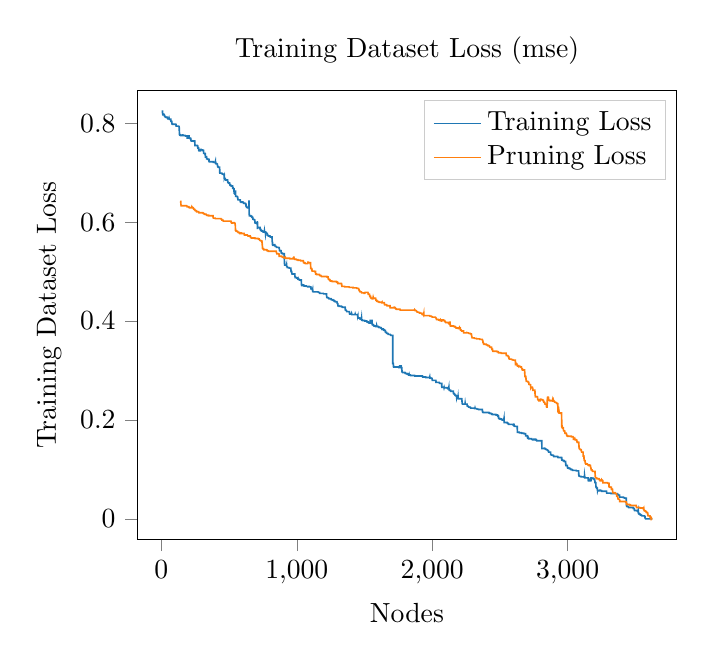
\begin{tikzpicture}

\definecolor{color0}{rgb}{0.12156862745098,0.466666666666667,0.705882352941177}
\definecolor{color1}{rgb}{1,0.498039215686275,0.0549019607843137}

\begin{axis}[
title={Training Dataset Loss (mse)},
xlabel={Nodes},
ylabel={Training Dataset Loss},
xmin=-179.15, xmax=3806.15,
ymin=-0.0412, ymax=0.8652,
tick align=outside,
tick pos=left,
x grid style={white!69.01960784313725!black},
y grid style={white!69.01960784313725!black},
legend cell align={left},
legend style={draw=white!80.0!black},
legend entries={{Training Loss},{Pruning Loss}}
]
\addlegendimage{no markers, color0}
\addlegendimage{no markers, color1}
\addplot [semithick, color0]
table {%
2 0.824
3 0.824
4 0.824
5 0.824
6 0.824
7 0.824
8 0.824
9 0.819
10 0.819
11 0.817
12 0.817
13 0.817
14 0.817
15 0.817
16 0.818
17 0.818
18 0.818
19 0.817
20 0.817
21 0.817
22 0.815
23 0.815
25 0.814
26 0.814
27 0.813
28 0.813
29 0.813
30 0.813
31 0.813
32 0.812
33 0.812
34 0.812
35 0.812
36 0.812
37 0.812
38 0.812
39 0.812
40 0.812
41 0.812
42 0.812
43 0.812
44 0.812
45 0.81
46 0.81
47 0.809
48 0.809
50 0.809
51 0.809
52 0.809
53 0.809
54 0.809
55 0.809
56 0.809
57 0.81
58 0.809
59 0.808
60 0.808
61 0.808
62 0.808
63 0.808
64 0.808
66 0.808
67 0.808
68 0.808
69 0.808
70 0.804
71 0.804
72 0.804
73 0.804
74 0.804
75 0.804
76 0.803
77 0.803
78 0.799
79 0.799
80 0.799
81 0.799
82 0.798
83 0.798
84 0.798
85 0.798
86 0.798
87 0.798
88 0.798
89 0.798
90 0.798
91 0.798
92 0.798
93 0.798
94 0.798
95 0.798
96 0.798
97 0.798
98 0.798
99 0.798
100 0.798
102 0.798
103 0.798
105 0.798
106 0.797
107 0.797
108 0.797
109 0.794
110 0.794
111 0.794
112 0.794
113 0.794
114 0.794
115 0.794
116 0.794
117 0.794
118 0.794
119 0.794
122 0.794
123 0.794
125 0.794
126 0.794
127 0.794
130 0.793
131 0.793
133 0.781
134 0.777
135 0.777
136 0.776
137 0.776
138 0.776
139 0.776
140 0.776
141 0.775
142 0.775
143 0.775
144 0.775
145 0.775
146 0.775
147 0.775
150 0.775
151 0.775
152 0.775
153 0.775
154 0.775
155 0.776
156 0.776
157 0.776
159 0.776
160 0.775
161 0.775
162 0.775
163 0.775
164 0.775
165 0.775
166 0.775
167 0.775
169 0.775
170 0.775
171 0.775
173 0.775
174 0.775
175 0.775
176 0.775
178 0.774
179 0.774
180 0.774
181 0.774
182 0.774
183 0.774
184 0.774
185 0.774
186 0.774
187 0.774
188 0.774
189 0.774
190 0.773
191 0.77
192 0.77
193 0.774
194 0.774
195 0.774
197 0.774
198 0.774
199 0.774
200 0.774
201 0.774
202 0.774
203 0.774
204 0.774
205 0.77
206 0.77
207 0.77
209 0.77
210 0.77
211 0.769
212 0.769
213 0.769
214 0.769
215 0.769
216 0.769
217 0.769
218 0.765
219 0.765
220 0.765
221 0.765
222 0.765
223 0.764
224 0.764
227 0.764
228 0.764
229 0.764
230 0.764
231 0.764
232 0.764
233 0.764
234 0.764
235 0.764
237 0.764
238 0.764
239 0.764
240 0.764
241 0.764
243 0.764
244 0.764
245 0.764
246 0.764
247 0.76
248 0.755
249 0.755
250 0.755
251 0.755
253 0.755
254 0.755
255 0.755
256 0.755
257 0.755
258 0.755
260 0.755
261 0.755
263 0.755
264 0.755
265 0.755
266 0.755
268 0.754
269 0.75
270 0.75
271 0.75
272 0.75
273 0.75
274 0.75
275 0.75
276 0.746
277 0.746
278 0.744
279 0.744
280 0.744
281 0.744
282 0.744
283 0.744
284 0.744
285 0.744
286 0.744
287 0.744
288 0.744
290 0.744
291 0.747
292 0.747
293 0.747
294 0.746
295 0.746
296 0.746
297 0.746
298 0.746
299 0.746
300 0.746
301 0.746
303 0.746
304 0.746
305 0.746
306 0.745
307 0.745
308 0.745
309 0.745
310 0.745
311 0.745
312 0.739
313 0.739
314 0.739
315 0.739
317 0.739
318 0.739
319 0.739
320 0.739
321 0.738
322 0.738
323 0.738
324 0.738
325 0.73
326 0.733
327 0.732
328 0.732
329 0.732
330 0.732
331 0.732
332 0.732
333 0.732
334 0.728
335 0.728
336 0.728
337 0.728
338 0.728
339 0.728
340 0.728
341 0.727
342 0.727
343 0.727
344 0.727
345 0.727
346 0.727
348 0.727
350 0.727
351 0.727
352 0.723
353 0.723
354 0.722
355 0.722
356 0.722
357 0.722
358 0.722
359 0.722
360 0.722
361 0.722
362 0.722
363 0.722
364 0.722
365 0.722
366 0.722
367 0.722
368 0.722
369 0.722
370 0.722
371 0.722
372 0.722
373 0.722
374 0.722
375 0.722
376 0.722
377 0.722
378 0.722
379 0.722
380 0.722
381 0.722
382 0.722
383 0.721
384 0.721
385 0.721
386 0.721
387 0.721
388 0.721
389 0.721
390 0.721
391 0.721
392 0.721
393 0.721
394 0.721
395 0.721
396 0.721
397 0.721
399 0.723
400 0.719
401 0.719
403 0.719
404 0.718
405 0.718
408 0.718
409 0.718
410 0.718
412 0.717
413 0.717
414 0.715
415 0.713
416 0.712
417 0.712
418 0.712
419 0.712
420 0.711
421 0.711
422 0.711
424 0.711
425 0.711
427 0.711
428 0.711
430 0.711
431 0.7
432 0.699
433 0.699
434 0.699
435 0.699
436 0.699
437 0.699
438 0.699
439 0.699
441 0.699
442 0.699
443 0.699
446 0.699
447 0.698
448 0.698
449 0.698
450 0.698
452 0.697
453 0.697
454 0.697
456 0.697
457 0.697
458 0.697
459 0.697
460 0.696
461 0.696
462 0.696
463 0.696
464 0.691
465 0.692
466 0.688
467 0.688
468 0.688
469 0.688
470 0.688
471 0.688
472 0.688
473 0.686
474 0.685
475 0.685
476 0.685
478 0.685
480 0.685
481 0.685
482 0.685
483 0.685
484 0.685
485 0.685
486 0.685
487 0.685
488 0.685
489 0.685
490 0.681
491 0.68
492 0.68
493 0.68
494 0.68
495 0.68
497 0.679
498 0.679
499 0.679
500 0.679
501 0.679
502 0.679
504 0.679
505 0.676
506 0.675
507 0.675
508 0.675
509 0.675
510 0.674
511 0.674
513 0.674
514 0.674
515 0.674
516 0.673
517 0.673
518 0.673
519 0.673
520 0.673
521 0.673
522 0.673
523 0.673
525 0.673
526 0.673
527 0.669
528 0.669
529 0.669
530 0.669
531 0.669
532 0.668
533 0.667
534 0.667
535 0.667
536 0.667
537 0.659
538 0.659
539 0.659
540 0.658
541 0.658
542 0.658
543 0.657
544 0.657
545 0.657
546 0.657
547 0.664
548 0.656
549 0.652
550 0.652
551 0.652
552 0.652
553 0.652
554 0.652
555 0.652
556 0.652
557 0.652
558 0.652
559 0.652
560 0.652
561 0.651
562 0.651
563 0.651
564 0.647
565 0.646
566 0.646
567 0.645
568 0.645
569 0.645
570 0.645
571 0.645
573 0.645
574 0.645
575 0.645
577 0.645
578 0.645
579 0.645
581 0.645
582 0.645
583 0.641
584 0.641
585 0.641
586 0.641
587 0.641
588 0.641
589 0.64
590 0.64
591 0.64
592 0.64
594 0.64
595 0.64
596 0.64
597 0.64
598 0.641
599 0.641
600 0.641
601 0.641
602 0.64
603 0.64
604 0.64
605 0.64
607 0.638
608 0.638
609 0.638
610 0.638
612 0.638
613 0.638
614 0.638
616 0.638
617 0.638
618 0.638
620 0.637
621 0.637
622 0.637
624 0.637
625 0.633
626 0.633
627 0.633
629 0.63
630 0.63
631 0.63
632 0.63
633 0.63
634 0.63
635 0.63
636 0.63
637 0.629
638 0.629
639 0.629
640 0.629
642 0.629
644 0.629
645 0.629
646 0.629
647 0.644
648 0.616
649 0.616
650 0.613
651 0.613
652 0.613
654 0.613
655 0.613
657 0.613
658 0.613
659 0.613
660 0.613
661 0.612
662 0.612
664 0.612
666 0.612
667 0.612
668 0.61
669 0.61
670 0.61
671 0.61
673 0.61
674 0.61
676 0.606
677 0.606
678 0.606
680 0.606
681 0.605
682 0.605
684 0.605
686 0.605
689 0.604
690 0.604
691 0.6
692 0.598
693 0.598
694 0.598
695 0.598
696 0.598
697 0.598
698 0.598
700 0.598
701 0.599
702 0.599
703 0.599
704 0.597
705 0.597
706 0.597
707 0.597
708 0.597
709 0.602
710 0.586
711 0.589
712 0.589
713 0.589
715 0.589
716 0.589
717 0.589
718 0.589
719 0.589
720 0.589
721 0.589
722 0.589
723 0.589
724 0.589
725 0.589
726 0.589
728 0.589
729 0.585
730 0.585
731 0.585
733 0.585
734 0.585
735 0.583
736 0.583
737 0.583
738 0.583
739 0.583
740 0.583
741 0.583
742 0.582
743 0.582
744 0.582
745 0.582
746 0.582
748 0.581
749 0.581
750 0.581
751 0.581
752 0.58
753 0.58
754 0.58
755 0.58
756 0.58
757 0.58
758 0.58
760 0.58
761 0.582
762 0.58
763 0.58
766 0.58
767 0.58
768 0.58
769 0.577
770 0.579
771 0.579
772 0.579
774 0.579
776 0.577
777 0.577
778 0.577
780 0.577
781 0.577
782 0.577
783 0.574
784 0.574
785 0.573
786 0.573
787 0.573
788 0.573
790 0.573
792 0.572
793 0.572
794 0.572
795 0.572
796 0.572
797 0.572
798 0.572
799 0.572
801 0.572
802 0.571
803 0.571
804 0.57
805 0.57
806 0.57
807 0.57
808 0.57
809 0.57
810 0.57
811 0.57
812 0.57
813 0.57
815 0.57
816 0.57
817 0.57
818 0.561
819 0.561
820 0.559
821 0.554
822 0.554
823 0.554
824 0.553
825 0.553
827 0.553
828 0.553
829 0.553
831 0.553
832 0.553
833 0.553
834 0.553
835 0.553
836 0.553
837 0.556
838 0.553
839 0.552
840 0.551
841 0.551
842 0.551
843 0.551
844 0.551
845 0.551
846 0.551
848 0.551
849 0.55
850 0.55
851 0.549
852 0.549
853 0.549
854 0.549
855 0.549
856 0.549
857 0.549
858 0.549
859 0.549
860 0.549
861 0.549
862 0.549
863 0.549
864 0.549
866 0.549
867 0.549
868 0.548
869 0.548
870 0.548
872 0.544
873 0.542
874 0.542
875 0.542
876 0.542
878 0.542
880 0.542
881 0.542
882 0.542
883 0.542
884 0.542
885 0.538
886 0.537
887 0.537
888 0.537
889 0.537
890 0.537
891 0.537
892 0.537
893 0.537
894 0.537
895 0.536
896 0.536
897 0.536
898 0.536
900 0.536
901 0.536
902 0.536
903 0.536
904 0.536
905 0.536
906 0.536
907 0.536
908 0.523
909 0.519
910 0.513
911 0.513
912 0.513
913 0.513
914 0.513
915 0.513
916 0.513
917 0.513
919 0.513
920 0.513
921 0.513
922 0.513
923 0.513
924 0.514
925 0.51
926 0.51
927 0.51
928 0.51
929 0.51
930 0.51
931 0.508
933 0.508
934 0.508
935 0.508
936 0.508
937 0.508
938 0.508
939 0.508
940 0.508
941 0.508
943 0.508
944 0.507
945 0.507
946 0.507
947 0.507
948 0.507
949 0.507
950 0.507
951 0.507
953 0.507
954 0.507
955 0.507
956 0.507
957 0.501
958 0.5
959 0.5
960 0.5
962 0.5
964 0.496
965 0.495
967 0.495
968 0.495
969 0.495
970 0.495
971 0.495
972 0.495
973 0.495
975 0.495
976 0.495
979 0.495
980 0.495
981 0.495
982 0.495
983 0.495
984 0.495
985 0.495
986 0.491
987 0.49
988 0.488
989 0.488
990 0.488
991 0.488
992 0.488
993 0.488
994 0.488
996 0.488
998 0.488
999 0.487
1000 0.487
1001 0.487
1002 0.487
1003 0.487
1006 0.486
1007 0.485
1008 0.485
1010 0.486
1011 0.485
1012 0.485
1013 0.484
1014 0.484
1015 0.484
1017 0.484
1018 0.484
1019 0.484
1021 0.483
1022 0.483
1024 0.483
1025 0.483
1026 0.483
1028 0.483
1029 0.483
1030 0.483
1033 0.483
1034 0.476
1035 0.473
1036 0.472
1037 0.472
1038 0.472
1040 0.472
1041 0.472
1043 0.472
1044 0.472
1045 0.472
1046 0.473
1047 0.473
1048 0.473
1049 0.473
1050 0.473
1051 0.472
1052 0.472
1053 0.471
1054 0.471
1055 0.471
1056 0.471
1057 0.471
1058 0.471
1059 0.471
1060 0.471
1061 0.471
1062 0.471
1063 0.471
1064 0.471
1067 0.471
1068 0.471
1069 0.471
1070 0.47
1071 0.47
1073 0.47
1074 0.47
1075 0.47
1077 0.47
1079 0.47
1080 0.47
1081 0.47
1082 0.469
1083 0.469
1084 0.469
1085 0.469
1086 0.469
1087 0.469
1088 0.469
1089 0.469
1090 0.469
1091 0.469
1092 0.47
1093 0.47
1094 0.469
1095 0.469
1096 0.469
1097 0.469
1098 0.469
1099 0.469
1100 0.469
1101 0.469
1102 0.469
1103 0.469
1104 0.469
1105 0.465
1106 0.465
1107 0.465
1108 0.465
1109 0.465
1110 0.465
1112 0.465
1114 0.464
1115 0.463
1116 0.463
1117 0.464
1118 0.46
1119 0.46
1121 0.459
1122 0.459
1123 0.459
1124 0.459
1125 0.459
1126 0.459
1127 0.459
1128 0.459
1129 0.459
1130 0.459
1131 0.459
1132 0.459
1135 0.459
1137 0.459
1138 0.459
1139 0.459
1141 0.459
1142 0.459
1143 0.459
1144 0.459
1146 0.459
1149 0.459
1150 0.459
1151 0.459
1153 0.459
1154 0.459
1156 0.459
1157 0.459
1160 0.458
1161 0.458
1162 0.458
1163 0.458
1164 0.458
1166 0.458
1167 0.458
1168 0.458
1169 0.456
1170 0.456
1171 0.456
1172 0.456
1173 0.456
1174 0.456
1175 0.456
1176 0.456
1177 0.456
1178 0.456
1179 0.456
1180 0.456
1181 0.456
1182 0.456
1183 0.456
1184 0.456
1186 0.456
1187 0.456
1188 0.456
1189 0.456
1190 0.456
1191 0.456
1192 0.456
1193 0.456
1195 0.456
1196 0.456
1198 0.455
1199 0.455
1201 0.455
1202 0.455
1203 0.455
1204 0.455
1206 0.455
1207 0.455
1208 0.455
1209 0.455
1210 0.455
1211 0.455
1213 0.455
1214 0.455
1216 0.455
1217 0.455
1218 0.455
1219 0.455
1220 0.451
1221 0.449
1222 0.448
1223 0.448
1224 0.448
1226 0.447
1227 0.447
1228 0.447
1230 0.447
1231 0.447
1232 0.447
1233 0.447
1234 0.447
1237 0.446
1238 0.445
1239 0.445
1240 0.445
1241 0.445
1242 0.445
1244 0.445
1245 0.445
1247 0.445
1248 0.445
1249 0.445
1251 0.445
1252 0.445
1253 0.445
1254 0.444
1255 0.443
1256 0.443
1258 0.443
1259 0.443
1260 0.443
1261 0.443
1262 0.443
1264 0.443
1265 0.443
1266 0.443
1267 0.442
1268 0.442
1269 0.442
1270 0.442
1272 0.442
1273 0.442
1274 0.442
1275 0.441
1276 0.44
1277 0.44
1278 0.44
1279 0.44
1280 0.44
1281 0.44
1282 0.44
1283 0.44
1284 0.439
1285 0.439
1286 0.439
1287 0.439
1288 0.439
1289 0.439
1291 0.439
1293 0.439
1294 0.439
1296 0.439
1297 0.438
1298 0.436
1300 0.435
1301 0.435
1302 0.435
1303 0.435
1304 0.431
1305 0.431
1307 0.431
1308 0.431
1309 0.431
1310 0.431
1311 0.431
1312 0.43
1313 0.43
1314 0.43
1315 0.43
1317 0.43
1318 0.43
1320 0.43
1321 0.43
1322 0.43
1323 0.43
1324 0.43
1326 0.43
1327 0.43
1328 0.43
1329 0.43
1330 0.429
1331 0.429
1333 0.429
1334 0.429
1335 0.429
1337 0.428
1338 0.428
1339 0.428
1340 0.428
1341 0.428
1342 0.428
1343 0.428
1344 0.428
1345 0.428
1347 0.428
1348 0.428
1349 0.428
1350 0.428
1351 0.428
1352 0.428
1354 0.428
1357 0.428
1358 0.424
1359 0.422
1360 0.422
1361 0.422
1362 0.422
1364 0.422
1367 0.42
1368 0.42
1369 0.419
1370 0.419
1371 0.419
1373 0.419
1374 0.419
1375 0.419
1376 0.419
1377 0.419
1378 0.419
1379 0.419
1380 0.419
1381 0.419
1382 0.419
1383 0.419
1384 0.419
1386 0.419
1387 0.419
1388 0.419
1389 0.418
1390 0.414
1391 0.414
1392 0.414
1393 0.415
1394 0.415
1395 0.415
1396 0.415
1397 0.415
1399 0.415
1400 0.414
1401 0.414
1402 0.414
1404 0.414
1405 0.415
1406 0.414
1407 0.413
1408 0.413
1410 0.413
1411 0.413
1412 0.413
1413 0.413
1414 0.413
1416 0.413
1417 0.413
1418 0.413
1419 0.413
1420 0.413
1421 0.413
1422 0.413
1423 0.413
1424 0.413
1425 0.413
1426 0.413
1427 0.413
1428 0.413
1429 0.413
1430 0.413
1431 0.414
1432 0.413
1433 0.413
1434 0.413
1436 0.413
1437 0.413
1438 0.413
1439 0.413
1440 0.413
1441 0.413
1442 0.413
1443 0.413
1445 0.413
1446 0.413
1447 0.413
1448 0.413
1450 0.409
1451 0.41
1452 0.406
1453 0.406
1454 0.406
1455 0.406
1456 0.406
1457 0.406
1458 0.406
1459 0.406
1460 0.406
1461 0.406
1462 0.406
1463 0.406
1464 0.406
1465 0.406
1466 0.405
1467 0.405
1468 0.404
1469 0.404
1470 0.404
1472 0.404
1474 0.404
1475 0.404
1476 0.404
1477 0.404
1478 0.406
1479 0.402
1480 0.402
1481 0.402
1482 0.402
1484 0.402
1485 0.401
1486 0.401
1487 0.401
1488 0.401
1489 0.401
1491 0.401
1492 0.401
1493 0.401
1494 0.401
1495 0.401
1496 0.401
1497 0.401
1498 0.401
1499 0.401
1501 0.401
1502 0.4
1503 0.4
1504 0.4
1505 0.4
1507 0.4
1508 0.4
1509 0.4
1510 0.4
1511 0.4
1512 0.4
1513 0.4
1514 0.4
1516 0.4
1517 0.4
1518 0.399
1519 0.398
1520 0.398
1521 0.398
1522 0.398
1523 0.398
1524 0.398
1525 0.398
1526 0.398
1527 0.398
1528 0.397
1529 0.397
1530 0.397
1531 0.397
1532 0.397
1533 0.397
1534 0.396
1535 0.396
1537 0.396
1539 0.396
1540 0.396
1541 0.396
1542 0.401
1543 0.401
1544 0.401
1545 0.401
1546 0.401
1547 0.401
1548 0.401
1549 0.401
1550 0.401
1551 0.401
1552 0.401
1553 0.401
1554 0.401
1555 0.401
1556 0.393
1557 0.393
1558 0.393
1559 0.393
1560 0.393
1561 0.393
1562 0.393
1563 0.392
1564 0.392
1566 0.392
1567 0.391
1568 0.391
1569 0.391
1570 0.39
1571 0.39
1572 0.39
1574 0.39
1575 0.39
1576 0.39
1577 0.39
1578 0.39
1579 0.39
1580 0.39
1581 0.389
1582 0.389
1583 0.389
1585 0.389
1586 0.389
1587 0.389
1588 0.389
1589 0.389
1590 0.391
1591 0.39
1592 0.389
1593 0.389
1594 0.389
1595 0.389
1596 0.389
1598 0.389
1600 0.389
1601 0.389
1602 0.389
1603 0.388
1604 0.388
1605 0.388
1606 0.388
1607 0.388
1608 0.387
1609 0.387
1610 0.387
1611 0.387
1612 0.387
1613 0.387
1614 0.387
1615 0.387
1616 0.387
1617 0.387
1620 0.387
1621 0.386
1622 0.386
1623 0.386
1624 0.386
1627 0.384
1628 0.384
1629 0.383
1630 0.383
1632 0.383
1633 0.384
1634 0.384
1635 0.384
1638 0.384
1639 0.384
1641 0.383
1642 0.383
1643 0.382
1644 0.382
1645 0.382
1646 0.382
1647 0.381
1648 0.381
1650 0.381
1651 0.381
1654 0.381
1655 0.378
1656 0.378
1657 0.377
1658 0.377
1659 0.377
1660 0.377
1661 0.377
1662 0.377
1663 0.377
1664 0.375
1665 0.375
1668 0.375
1669 0.375
1670 0.375
1671 0.375
1672 0.375
1673 0.375
1674 0.374
1675 0.373
1676 0.373
1677 0.373
1678 0.373
1679 0.373
1680 0.373
1681 0.373
1682 0.373
1683 0.373
1684 0.373
1685 0.373
1686 0.373
1687 0.373
1690 0.373
1691 0.372
1692 0.372
1693 0.372
1694 0.371
1695 0.371
1696 0.371
1698 0.371
1699 0.371
1701 0.371
1702 0.371
1703 0.371
1704 0.371
1705 0.371
1706 0.371
1707 0.371
1708 0.371
1709 0.314
1710 0.314
1711 0.314
1712 0.314
1713 0.314
1714 0.308
1715 0.308
1716 0.307
1717 0.307
1718 0.307
1719 0.307
1720 0.307
1721 0.307
1722 0.307
1723 0.307
1724 0.307
1725 0.307
1726 0.307
1728 0.307
1729 0.307
1730 0.307
1732 0.307
1733 0.307
1735 0.307
1736 0.307
1737 0.307
1738 0.307
1739 0.307
1740 0.307
1741 0.307
1743 0.307
1744 0.307
1745 0.307
1746 0.307
1747 0.307
1748 0.307
1749 0.307
1750 0.307
1751 0.307
1752 0.307
1753 0.306
1754 0.306
1756 0.306
1758 0.306
1759 0.309
1760 0.309
1761 0.309
1762 0.309
1763 0.309
1765 0.309
1766 0.309
1767 0.309
1768 0.309
1771 0.309
1773 0.305
1774 0.305
1775 0.305
1776 0.299
1777 0.299
1778 0.297
1779 0.297
1781 0.296
1782 0.296
1783 0.296
1786 0.296
1787 0.296
1788 0.296
1789 0.296
1790 0.296
1791 0.296
1792 0.296
1794 0.296
1795 0.296
1796 0.296
1797 0.296
1798 0.296
1799 0.295
1800 0.295
1801 0.295
1802 0.294
1803 0.294
1804 0.294
1805 0.294
1808 0.294
1809 0.294
1810 0.294
1811 0.294
1812 0.294
1813 0.294
1814 0.293
1815 0.293
1816 0.293
1818 0.293
1819 0.293
1820 0.293
1823 0.292
1824 0.292
1825 0.291
1826 0.291
1827 0.291
1828 0.291
1829 0.291
1830 0.292
1831 0.291
1832 0.291
1833 0.291
1834 0.291
1835 0.291
1836 0.291
1837 0.291
1838 0.291
1839 0.29
1840 0.29
1841 0.29
1842 0.29
1843 0.29
1844 0.29
1845 0.29
1846 0.29
1847 0.29
1848 0.29
1850 0.29
1851 0.29
1852 0.29
1853 0.29
1855 0.29
1856 0.29
1857 0.29
1859 0.29
1860 0.29
1861 0.29
1863 0.29
1864 0.29
1865 0.29
1866 0.29
1867 0.29
1868 0.29
1869 0.29
1871 0.29
1872 0.289
1873 0.289
1874 0.289
1875 0.289
1876 0.289
1877 0.289
1878 0.289
1879 0.289
1880 0.289
1881 0.289
1882 0.289
1884 0.289
1885 0.289
1886 0.289
1887 0.289
1888 0.289
1889 0.289
1890 0.289
1891 0.289
1892 0.289
1894 0.289
1895 0.289
1897 0.289
1898 0.289
1899 0.289
1901 0.289
1902 0.289
1903 0.289
1904 0.289
1905 0.289
1906 0.289
1908 0.289
1909 0.289
1910 0.289
1911 0.289
1912 0.289
1913 0.289
1914 0.289
1915 0.289
1916 0.289
1918 0.289
1919 0.289
1920 0.289
1921 0.289
1922 0.289
1923 0.289
1925 0.289
1926 0.289
1928 0.289
1929 0.287
1930 0.287
1931 0.287
1932 0.287
1933 0.287
1935 0.287
1937 0.287
1938 0.287
1940 0.287
1941 0.287
1942 0.287
1943 0.287
1945 0.287
1947 0.287
1948 0.287
1949 0.287
1950 0.287
1952 0.287
1953 0.286
1954 0.286
1955 0.286
1956 0.286
1957 0.286
1958 0.286
1960 0.286
1961 0.286
1962 0.286
1963 0.286
1964 0.286
1965 0.286
1966 0.286
1967 0.286
1968 0.286
1969 0.286
1970 0.286
1971 0.286
1972 0.286
1973 0.286
1975 0.286
1976 0.286
1978 0.286
1979 0.286
1980 0.286
1981 0.286
1982 0.287
1983 0.285
1984 0.285
1985 0.285
1986 0.285
1988 0.285
1989 0.285
1990 0.285
1991 0.285
1993 0.284
1995 0.284
1996 0.284
1997 0.284
1998 0.284
1999 0.284
2000 0.281
2001 0.28
2002 0.28
2003 0.28
2004 0.28
2005 0.28
2006 0.28
2007 0.28
2008 0.28
2009 0.28
2010 0.28
2012 0.28
2013 0.28
2014 0.28
2015 0.28
2016 0.28
2017 0.28
2018 0.28
2019 0.28
2021 0.28
2022 0.28
2024 0.28
2026 0.28
2027 0.28
2028 0.276
2029 0.276
2030 0.276
2031 0.276
2032 0.276
2033 0.276
2034 0.276
2035 0.276
2036 0.276
2037 0.276
2039 0.276
2040 0.276
2041 0.276
2043 0.276
2044 0.276
2045 0.276
2047 0.276
2048 0.276
2049 0.276
2050 0.276
2051 0.276
2052 0.276
2053 0.275
2054 0.275
2055 0.274
2056 0.274
2057 0.274
2058 0.274
2059 0.274
2060 0.274
2061 0.274
2062 0.274
2063 0.274
2064 0.274
2065 0.274
2066 0.274
2067 0.274
2068 0.274
2070 0.274
2071 0.266
2072 0.266
2073 0.266
2074 0.266
2075 0.266
2076 0.266
2077 0.266
2078 0.266
2079 0.266
2080 0.266
2081 0.266
2082 0.266
2083 0.266
2084 0.266
2085 0.266
2086 0.266
2087 0.265
2088 0.266
2089 0.265
2090 0.265
2091 0.265
2092 0.265
2093 0.265
2094 0.265
2095 0.265
2096 0.265
2097 0.265
2098 0.265
2099 0.265
2100 0.265
2101 0.265
2102 0.265
2103 0.265
2105 0.265
2106 0.265
2107 0.265
2108 0.265
2109 0.265
2110 0.265
2111 0.264
2112 0.264
2113 0.264
2114 0.264
2116 0.263
2117 0.263
2118 0.263
2120 0.263
2121 0.263
2123 0.266
2124 0.262
2125 0.261
2126 0.26
2127 0.26
2128 0.26
2129 0.26
2130 0.26
2131 0.26
2132 0.26
2133 0.26
2134 0.26
2135 0.26
2136 0.26
2137 0.258
2138 0.258
2139 0.258
2140 0.258
2143 0.258
2144 0.258
2146 0.258
2147 0.258
2148 0.258
2149 0.258
2152 0.258
2154 0.258
2155 0.258
2156 0.258
2157 0.254
2158 0.254
2159 0.254
2160 0.253
2161 0.253
2162 0.253
2163 0.253
2164 0.253
2165 0.253
2167 0.251
2168 0.25
2169 0.25
2170 0.25
2171 0.25
2172 0.25
2173 0.25
2174 0.249
2175 0.249
2176 0.249
2177 0.249
2178 0.249
2179 0.249
2180 0.249
2181 0.245
2182 0.246
2183 0.246
2185 0.246
2188 0.245
2189 0.245
2190 0.245
2191 0.247
2192 0.244
2193 0.243
2194 0.243
2195 0.243
2197 0.243
2198 0.243
2199 0.243
2200 0.243
2201 0.243
2203 0.243
2204 0.243
2206 0.243
2207 0.243
2208 0.243
2210 0.243
2211 0.243
2212 0.243
2214 0.243
2216 0.243
2217 0.243
2218 0.243
2220 0.238
2221 0.235
2222 0.233
2223 0.233
2224 0.232
2225 0.232
2226 0.232
2227 0.232
2228 0.232
2230 0.232
2231 0.232
2232 0.232
2233 0.232
2234 0.232
2235 0.232
2236 0.232
2237 0.232
2238 0.232
2239 0.232
2240 0.232
2241 0.232
2242 0.232
2243 0.234
2244 0.232
2245 0.232
2246 0.232
2248 0.232
2249 0.232
2250 0.232
2251 0.232
2252 0.232
2253 0.232
2255 0.232
2256 0.232
2257 0.232
2258 0.23
2259 0.228
2260 0.228
2262 0.228
2263 0.228
2264 0.228
2265 0.228
2267 0.227
2268 0.227
2269 0.226
2270 0.226
2271 0.226
2272 0.226
2273 0.226
2274 0.226
2276 0.226
2279 0.226
2281 0.226
2282 0.226
2283 0.224
2284 0.224
2285 0.224
2286 0.224
2287 0.224
2288 0.224
2289 0.224
2291 0.224
2292 0.224
2293 0.224
2294 0.224
2295 0.224
2296 0.224
2298 0.224
2299 0.224
2300 0.224
2301 0.224
2302 0.224
2303 0.224
2304 0.224
2305 0.224
2306 0.224
2307 0.224
2308 0.224
2309 0.224
2310 0.224
2311 0.224
2312 0.223
2313 0.223
2314 0.223
2315 0.223
2316 0.224
2317 0.223
2318 0.223
2320 0.223
2321 0.223
2322 0.223
2323 0.223
2324 0.223
2325 0.223
2327 0.223
2329 0.223
2331 0.222
2333 0.222
2334 0.222
2335 0.222
2336 0.222
2338 0.222
2339 0.222
2340 0.222
2341 0.222
2342 0.222
2343 0.221
2344 0.221
2346 0.221
2349 0.221
2350 0.221
2352 0.221
2353 0.221
2355 0.221
2356 0.221
2357 0.221
2358 0.221
2359 0.221
2361 0.221
2362 0.221
2364 0.221
2366 0.221
2368 0.221
2369 0.221
2370 0.221
2372 0.216
2373 0.216
2374 0.216
2376 0.215
2377 0.215
2379 0.215
2381 0.215
2382 0.215
2383 0.215
2384 0.215
2385 0.215
2386 0.215
2387 0.215
2388 0.215
2389 0.215
2390 0.215
2391 0.215
2392 0.215
2393 0.215
2394 0.215
2395 0.215
2397 0.215
2398 0.215
2399 0.215
2400 0.215
2401 0.215
2402 0.215
2403 0.215
2404 0.215
2405 0.215
2406 0.215
2408 0.215
2409 0.215
2410 0.215
2411 0.215
2412 0.215
2413 0.215
2414 0.215
2415 0.215
2416 0.215
2417 0.215
2418 0.215
2419 0.215
2420 0.214
2421 0.214
2422 0.214
2423 0.214
2424 0.214
2425 0.214
2427 0.213
2428 0.213
2429 0.213
2430 0.213
2433 0.213
2434 0.213
2435 0.213
2436 0.213
2437 0.213
2438 0.213
2439 0.212
2440 0.212
2441 0.212
2442 0.212
2443 0.211
2444 0.211
2445 0.211
2446 0.211
2447 0.211
2449 0.211
2450 0.211
2451 0.211
2452 0.211
2453 0.211
2454 0.211
2456 0.211
2457 0.211
2458 0.211
2459 0.211
2460 0.211
2462 0.211
2463 0.211
2464 0.211
2465 0.211
2467 0.211
2469 0.211
2470 0.211
2471 0.211
2472 0.21
2473 0.21
2474 0.21
2475 0.21
2476 0.21
2477 0.21
2478 0.21
2479 0.21
2480 0.21
2481 0.21
2482 0.21
2483 0.21
2484 0.208
2485 0.208
2486 0.208
2488 0.208
2489 0.208
2490 0.204
2491 0.204
2492 0.203
2493 0.203
2494 0.203
2495 0.203
2496 0.203
2497 0.203
2499 0.203
2500 0.202
2502 0.202
2503 0.202
2504 0.202
2505 0.202
2506 0.202
2507 0.202
2508 0.202
2510 0.202
2511 0.201
2512 0.201
2513 0.201
2514 0.201
2516 0.201
2517 0.2
2518 0.2
2519 0.2
2520 0.2
2522 0.2
2523 0.2
2524 0.2
2525 0.2
2526 0.2
2527 0.2
2528 0.2
2530 0.203
2531 0.195
2532 0.195
2533 0.195
2534 0.195
2535 0.195
2536 0.195
2537 0.195
2538 0.195
2539 0.195
2540 0.195
2541 0.195
2542 0.195
2543 0.195
2545 0.195
2546 0.195
2547 0.195
2548 0.195
2549 0.195
2552 0.195
2553 0.195
2554 0.194
2555 0.194
2556 0.194
2557 0.193
2558 0.193
2559 0.193
2560 0.193
2561 0.193
2563 0.193
2564 0.191
2565 0.191
2566 0.191
2567 0.191
2570 0.191
2571 0.191
2572 0.191
2573 0.191
2574 0.191
2575 0.191
2576 0.191
2577 0.191
2578 0.191
2579 0.191
2580 0.191
2581 0.191
2583 0.191
2584 0.191
2585 0.191
2587 0.191
2588 0.191
2589 0.191
2590 0.191
2591 0.191
2593 0.191
2594 0.191
2595 0.191
2596 0.19
2597 0.19
2598 0.19
2600 0.19
2601 0.19
2602 0.19
2603 0.193
2604 0.188
2605 0.188
2606 0.188
2607 0.188
2608 0.188
2611 0.187
2612 0.187
2614 0.187
2615 0.187
2616 0.187
2618 0.187
2619 0.187
2620 0.187
2621 0.187
2623 0.187
2624 0.187
2625 0.187
2626 0.187
2628 0.187
2629 0.175
2630 0.175
2631 0.175
2632 0.175
2633 0.175
2634 0.175
2635 0.175
2636 0.175
2637 0.175
2638 0.175
2639 0.175
2640 0.175
2641 0.175
2642 0.175
2643 0.175
2644 0.174
2645 0.174
2646 0.174
2647 0.174
2648 0.174
2649 0.174
2650 0.174
2651 0.174
2652 0.174
2653 0.174
2654 0.174
2656 0.174
2657 0.174
2658 0.174
2659 0.174
2660 0.174
2661 0.173
2662 0.173
2663 0.173
2664 0.173
2665 0.173
2666 0.173
2667 0.173
2668 0.173
2669 0.173
2670 0.173
2671 0.173
2672 0.173
2673 0.173
2674 0.173
2676 0.173
2677 0.173
2679 0.172
2680 0.172
2681 0.172
2682 0.172
2683 0.172
2684 0.172
2685 0.172
2687 0.172
2689 0.172
2690 0.168
2692 0.168
2693 0.168
2694 0.168
2695 0.168
2696 0.168
2698 0.168
2699 0.168
2700 0.168
2701 0.168
2702 0.168
2703 0.168
2704 0.164
2705 0.163
2706 0.163
2707 0.163
2709 0.164
2710 0.163
2711 0.163
2712 0.163
2713 0.162
2714 0.162
2716 0.162
2717 0.162
2718 0.162
2719 0.162
2720 0.162
2721 0.162
2722 0.162
2723 0.162
2724 0.162
2725 0.162
2726 0.162
2727 0.162
2728 0.162
2729 0.162
2730 0.162
2731 0.162
2733 0.162
2735 0.162
2736 0.161
2737 0.161
2741 0.16
2742 0.16
2743 0.16
2744 0.16
2746 0.16
2747 0.16
2749 0.16
2750 0.161
2751 0.161
2752 0.16
2753 0.16
2754 0.16
2755 0.16
2756 0.16
2758 0.16
2760 0.16
2761 0.16
2762 0.16
2763 0.161
2764 0.161
2765 0.161
2766 0.16
2767 0.16
2768 0.159
2769 0.159
2770 0.159
2772 0.159
2773 0.158
2774 0.158
2775 0.158
2776 0.158
2777 0.158
2779 0.158
2780 0.158
2781 0.158
2783 0.158
2784 0.158
2785 0.158
2786 0.158
2787 0.158
2788 0.158
2789 0.158
2791 0.158
2792 0.158
2795 0.158
2796 0.158
2797 0.158
2798 0.158
2799 0.158
2800 0.158
2801 0.158
2802 0.158
2803 0.158
2804 0.158
2805 0.158
2806 0.158
2807 0.158
2808 0.158
2809 0.158
2810 0.142
2811 0.142
2812 0.142
2813 0.142
2814 0.142
2815 0.142
2816 0.142
2817 0.142
2818 0.142
2820 0.142
2822 0.142
2823 0.142
2824 0.142
2825 0.142
2826 0.143
2827 0.143
2829 0.143
2830 0.143
2831 0.143
2833 0.142
2834 0.142
2835 0.141
2836 0.141
2837 0.141
2838 0.141
2839 0.141
2840 0.141
2841 0.141
2842 0.14
2843 0.14
2845 0.14
2846 0.14
2848 0.14
2850 0.139
2851 0.139
2852 0.139
2853 0.139
2854 0.138
2855 0.138
2856 0.138
2858 0.138
2860 0.135
2861 0.135
2862 0.135
2863 0.135
2864 0.135
2865 0.135
2866 0.135
2867 0.135
2868 0.135
2869 0.135
2870 0.135
2872 0.135
2873 0.135
2874 0.135
2875 0.13
2876 0.13
2877 0.13
2878 0.13
2879 0.13
2880 0.13
2881 0.129
2882 0.129
2883 0.129
2884 0.129
2885 0.129
2886 0.129
2887 0.129
2888 0.129
2889 0.129
2890 0.129
2891 0.129
2892 0.128
2893 0.128
2894 0.128
2895 0.128
2896 0.128
2898 0.126
2899 0.126
2900 0.126
2901 0.126
2902 0.126
2903 0.126
2904 0.126
2905 0.126
2906 0.126
2907 0.126
2908 0.126
2909 0.126
2910 0.126
2912 0.126
2914 0.126
2915 0.126
2916 0.126
2917 0.126
2918 0.126
2920 0.126
2921 0.126
2923 0.126
2924 0.126
2925 0.126
2927 0.126
2929 0.124
2930 0.124
2931 0.124
2932 0.124
2933 0.124
2934 0.124
2935 0.124
2936 0.124
2937 0.124
2938 0.124
2939 0.124
2940 0.124
2941 0.124
2943 0.124
2944 0.124
2945 0.124
2947 0.124
2948 0.124
2949 0.124
2950 0.124
2951 0.124
2952 0.124
2953 0.124
2955 0.124
2956 0.124
2957 0.119
2958 0.119
2959 0.119
2960 0.119
2961 0.119
2962 0.119
2964 0.118
2965 0.118
2966 0.118
2967 0.118
2968 0.118
2969 0.118
2971 0.118
2972 0.118
2973 0.117
2974 0.117
2975 0.116
2976 0.116
2977 0.116
2978 0.116
2979 0.116
2980 0.116
2981 0.116
2982 0.116
2983 0.116
2984 0.116
2985 0.116
2986 0.11
2987 0.108
2988 0.108
2989 0.108
2990 0.108
2991 0.108
2992 0.108
2993 0.108
2996 0.108
2998 0.108
2999 0.104
3000 0.103
3001 0.103
3002 0.103
3004 0.103
3005 0.103
3006 0.103
3007 0.103
3009 0.103
3010 0.103
3011 0.102
3012 0.102
3013 0.102
3014 0.102
3015 0.102
3016 0.102
3017 0.102
3018 0.102
3019 0.102
3020 0.101
3021 0.101
3022 0.101
3023 0.101
3024 0.1
3025 0.1
3026 0.1
3027 0.1
3028 0.1
3029 0.1
3030 0.1
3031 0.1
3032 0.1
3033 0.099
3034 0.099
3035 0.099
3036 0.099
3037 0.098
3038 0.098
3039 0.098
3040 0.098
3041 0.098
3043 0.098
3044 0.098
3045 0.098
3046 0.098
3047 0.098
3048 0.098
3049 0.098
3050 0.098
3052 0.098
3053 0.098
3054 0.098
3055 0.098
3056 0.098
3057 0.098
3060 0.098
3061 0.098
3062 0.098
3063 0.098
3064 0.097
3065 0.097
3066 0.097
3067 0.097
3068 0.097
3069 0.097
3070 0.097
3072 0.097
3073 0.097
3074 0.097
3076 0.097
3077 0.097
3078 0.097
3079 0.097
3080 0.097
3081 0.097
3082 0.09
3083 0.09
3084 0.087
3085 0.087
3086 0.087
3089 0.086
3091 0.086
3093 0.086
3095 0.086
3097 0.086
3099 0.086
3100 0.085
3102 0.085
3103 0.085
3104 0.085
3105 0.085
3108 0.085
3110 0.085
3111 0.085
3114 0.085
3116 0.085
3118 0.085
3120 0.085
3121 0.084
3122 0.084
3123 0.084
3124 0.084
3125 0.088
3126 0.086
3127 0.083
3128 0.083
3129 0.083
3131 0.083
3132 0.083
3133 0.083
3135 0.083
3137 0.083
3138 0.083
3140 0.083
3141 0.083
3142 0.083
3143 0.083
3144 0.083
3145 0.083
3146 0.083
3147 0.083
3149 0.083
3150 0.083
3151 0.083
3152 0.081
3153 0.077
3154 0.077
3155 0.077
3156 0.077
3157 0.077
3158 0.077
3159 0.077
3160 0.077
3161 0.077
3163 0.077
3164 0.077
3165 0.078
3166 0.077
3167 0.077
3168 0.077
3169 0.077
3170 0.077
3172 0.077
3173 0.083
3174 0.083
3175 0.083
3176 0.083
3177 0.083
3178 0.083
3179 0.082
3180 0.082
3181 0.082
3182 0.082
3183 0.082
3185 0.082
3187 0.082
3188 0.082
3189 0.082
3190 0.081
3191 0.081
3192 0.081
3194 0.081
3195 0.081
3196 0.08
3197 0.08
3198 0.08
3199 0.08
3200 0.079
3202 0.074
3203 0.074
3204 0.073
3205 0.073
3206 0.073
3207 0.073
3208 0.073
3209 0.065
3210 0.065
3211 0.065
3212 0.065
3213 0.064
3214 0.062
3215 0.062
3216 0.062
3217 0.062
3218 0.062
3219 0.062
3220 0.06
3221 0.057
3222 0.058
3223 0.057
3224 0.057
3225 0.057
3226 0.057
3227 0.057
3228 0.057
3229 0.057
3231 0.057
3232 0.057
3233 0.057
3234 0.057
3235 0.057
3237 0.058
3238 0.058
3239 0.058
3240 0.058
3241 0.058
3242 0.058
3243 0.058
3244 0.057
3245 0.057
3246 0.057
3248 0.057
3249 0.057
3250 0.057
3251 0.057
3252 0.056
3253 0.056
3255 0.056
3256 0.056
3257 0.056
3258 0.056
3259 0.056
3260 0.056
3261 0.056
3263 0.056
3265 0.056
3266 0.056
3267 0.056
3268 0.056
3269 0.056
3270 0.056
3271 0.056
3272 0.056
3273 0.056
3274 0.056
3275 0.056
3276 0.056
3277 0.056
3278 0.056
3279 0.056
3280 0.056
3281 0.056
3282 0.056
3283 0.056
3284 0.056
3285 0.056
3286 0.056
3287 0.056
3288 0.054
3289 0.052
3290 0.052
3291 0.052
3292 0.052
3293 0.052
3294 0.052
3295 0.052
3297 0.052
3298 0.052
3299 0.052
3301 0.052
3302 0.052
3303 0.052
3304 0.052
3305 0.052
3306 0.052
3310 0.052
3312 0.052
3313 0.052
3314 0.052
3315 0.052
3316 0.052
3317 0.052
3319 0.052
3320 0.051
3321 0.051
3324 0.051
3326 0.051
3327 0.051
3328 0.051
3329 0.051
3330 0.051
3331 0.051
3332 0.051
3334 0.051
3335 0.051
3336 0.051
3337 0.051
3338 0.051
3341 0.051
3342 0.051
3343 0.051
3344 0.051
3345 0.051
3346 0.051
3347 0.051
3348 0.051
3351 0.051
3353 0.051
3354 0.051
3355 0.051
3357 0.051
3358 0.051
3360 0.051
3361 0.051
3363 0.051
3365 0.051
3366 0.051
3367 0.051
3368 0.051
3369 0.05
3370 0.05
3372 0.049
3373 0.049
3374 0.049
3375 0.048
3376 0.048
3377 0.048
3378 0.048
3379 0.048
3380 0.048
3381 0.048
3382 0.048
3383 0.048
3384 0.044
3385 0.044
3386 0.044
3387 0.044
3388 0.044
3389 0.044
3390 0.044
3391 0.044
3392 0.044
3393 0.044
3395 0.044
3396 0.044
3397 0.044
3399 0.044
3400 0.044
3401 0.044
3402 0.044
3403 0.044
3404 0.044
3406 0.044
3407 0.044
3408 0.044
3409 0.044
3410 0.044
3411 0.044
3412 0.043
3413 0.043
3414 0.043
3415 0.043
3416 0.043
3417 0.043
3418 0.043
3419 0.043
3420 0.043
3421 0.042
3422 0.042
3423 0.042
3424 0.042
3425 0.042
3426 0.042
3428 0.042
3429 0.042
3430 0.042
3431 0.042
3432 0.042
3433 0.042
3434 0.032
3435 0.027
3436 0.027
3437 0.026
3438 0.026
3439 0.025
3440 0.025
3441 0.025
3442 0.025
3443 0.025
3444 0.025
3445 0.025
3447 0.025
3448 0.025
3449 0.024
3450 0.023
3451 0.023
3452 0.023
3453 0.023
3454 0.023
3455 0.023
3456 0.023
3457 0.023
3458 0.023
3459 0.023
3460 0.023
3461 0.023
3462 0.023
3463 0.023
3464 0.023
3466 0.023
3467 0.023
3468 0.023
3469 0.023
3470 0.023
3472 0.023
3473 0.023
3474 0.023
3475 0.023
3476 0.023
3478 0.023
3480 0.023
3481 0.023
3482 0.023
3483 0.023
3485 0.021
3486 0.021
3487 0.021
3488 0.021
3490 0.021
3491 0.021
3492 0.021
3493 0.019
3494 0.017
3495 0.017
3496 0.017
3499 0.017
3500 0.017
3501 0.017
3502 0.017
3503 0.017
3504 0.017
3505 0.017
3506 0.017
3509 0.017
3510 0.017
3511 0.017
3512 0.017
3513 0.017
3514 0.017
3515 0.016
3516 0.016
3517 0.016
3518 0.016
3520 0.016
3521 0.017
3522 0.011
3523 0.013
3524 0.011
3525 0.011
3526 0.011
3527 0.011
3528 0.01
3529 0.01
3530 0.01
3533 0.01
3534 0.009
3535 0.009
3536 0.009
3537 0.009
3538 0.008
3539 0.008
3540 0.008
3541 0.008
3543 0.008
3545 0.007
3546 0.007
3547 0.007
3548 0.007
3549 0.007
3550 0.006
3551 0.006
3552 0.006
3553 0.006
3554 0.006
3555 0.006
3556 0.006
3557 0.006
3559 0.006
3560 0.006
3561 0.006
3562 0.006
3563 0.006
3564 0.006
3565 0.006
3566 0.006
3567 0.006
3568 0.005
3569 0.005
3570 0.005
3571 0.005
3572 0.002
3573 0.001
3574 0.001
3577 0
3578 0
3579 0
3580 0
3582 0
3584 0
3585 0
3586 0
3587 0
3588 0
3589 0
3590 0
3592 0
3594 0
3595 0
3596 0
3597 0
3598 0
3599 0
3600 0
3601 0
3602 0
3603 0
3605 0
3606 0
3607 0
3608 0
3609 0
3610 0
3612 0
3613 0
3614 0
3615 0
3616 0
3617 0
3618 0
3619 0
3620 0
3621 0
3622 0
3623 0
3624 0
3625 0
};
\addplot [semithick, color1]
table {%
3625 0
3625 0
3623 0
3622 0
3622 0
3621 0
3621 0
3620 0
3619 0.001
3617 0
3615 0.002
3615 0.002
3614 0.002
3614 0.002
3614 0.002
3614 0.002
3612 0.002
3611 0.003
3609 0.003
3608 0.006
3605 0.006
3605 0.006
3604 0.006
3604 0.006
3603 0.006
3602 0.006
3602 0.006
3600 0.006
3598 0.006
3597 0.007
3597 0.007
3597 0.007
3595 0.007
3593 0.007
3591 0.012
3591 0.012
3590 0.012
3589 0.013
3589 0.013
3589 0.013
3588 0.013
3586 0.013
3584 0.013
3584 0.013
3583 0.013
3582 0.013
3580 0.015
3580 0.015
3580 0.015
3580 0.015
3579 0.015
3578 0.015
3576 0.015
3574 0.016
3574 0.016
3574 0.016
3573 0.016
3571 0.016
3569 0.017
3569 0.017
3569 0.017
3567 0.017
3566 0.017
3565 0.017
3565 0.017
3564 0.018
3562 0.022
3560 0.021
3558 0.021
3556 0.021
3556 0.021
3555 0.022
3555 0.022
3553 0.022
3553 0.022
3552 0.022
3552 0.022
3551 0.022
3549 0.022
3547 0.022
3547 0.022
3546 0.022
3545 0.022
3544 0.022
3544 0.022
3544 0.022
3544 0.022
3542 0.022
3542 0.022
3541 0.022
3540 0.022
3538 0.022
3536 0.022
3534 0.022
3534 0.022
3534 0.022
3532 0.023
3531 0.023
3530 0.023
3529 0.023
3529 0.023
3528 0.023
3528 0.023
3527 0.023
3526 0.023
3526 0.023
3526 0.023
3524 0.023
3524 0.023
3523 0.023
3522 0.023
3520 0.023
3518 0.023
3516 0.023
3516 0.023
3516 0.023
3514 0.023
3513 0.023
3512 0.023
3510 0.023
3510 0.023
3510 0.023
3508 0.024
3506 0.027
3505 0.027
3504 0.027
3504 0.027
3504 0.027
3502 0.027
3501 0.027
3501 0.027
3501 0.027
3500 0.027
3500 0.027
3498 0.027
3496 0.027
3495 0.027
3495 0.027
3494 0.027
3494 0.027
3493 0.027
3492 0.027
3491 0.027
3490 0.027
3490 0.027
3490 0.027
3488 0.027
3487 0.027
3487 0.027
3486 0.027
3486 0.027
3486 0.027
3485 0.027
3484 0.027
3483 0.027
3483 0.027
3481 0.027
3480 0.027
3480 0.027
3479 0.027
3479 0.027
3478 0.027
3478 0.027
3477 0.027
3475 0.027
3473 0.027
3471 0.027
3470 0.027
3470 0.027
3470 0.027
3469 0.027
3469 0.027
3469 0.027
3468 0.027
3467 0.027
3467 0.027
3466 0.027
3464 0.027
3462 0.027
3462 0.028
3460 0.028
3458 0.029
3457 0.029
3457 0.029
3456 0.029
3456 0.029
3455 0.029
3454 0.029
3454 0.029
3453 0.029
3453 0.029
3451 0.029
3449 0.029
3447 0.029
3447 0.029
3446 0.029
3446 0.029
3445 0.029
3443 0.029
3443 0.029
3443 0.029
3443 0.029
3441 0.029
3439 0.029
3438 0.03
3436 0.03
3435 0.03
3435 0.03
3434 0.034
3434 0.034
3432 0.034
3429 0.034
3429 0.034
3428 0.034
3428 0.034
3426 0.035
3426 0.035
3425 0.035
3423 0.035
3423 0.035
3423 0.035
3423 0.035
3421 0.035
3420 0.035
3420 0.035
3420 0.035
3419 0.035
3417 0.035
3417 0.035
3416 0.035
3414 0.035
3412 0.035
3410 0.035
3409 0.035
3409 0.035
3407 0.035
3405 0.035
3403 0.035
3403 0.035
3403 0.035
3403 0.035
3403 0.035
3401 0.035
3401 0.035
3401 0.035
3400 0.035
3398 0.035
3398 0.035
3397 0.035
3397 0.035
3397 0.035
3396 0.035
3394 0.035
3393 0.035
3391 0.035
3389 0.035
3388 0.035
3386 0.035
3386 0.035
3385 0.035
3384 0.039
3384 0.039
3383 0.039
3382 0.039
3380 0.04
3378 0.04
3378 0.04
3378 0.04
3378 0.04
3376 0.04
3376 0.04
3376 0.04
3374 0.04
3373 0.04
3371 0.042
3369 0.046
3369 0.046
3368 0.046
3367 0.046
3367 0.046
3365 0.046
3363 0.046
3361 0.051
3361 0.051
3361 0.051
3361 0.051
3361 0.051
3360 0.051
3360 0.051
3358 0.051
3356 0.051
3354 0.051
3352 0.052
3352 0.052
3351 0.052
3350 0.053
3350 0.053
3349 0.053
3348 0.053
3348 0.053
3345 0.053
3343 0.053
3343 0.053
3343 0.053
3341 0.053
3340 0.053
3340 0.053
3339 0.053
3338 0.053
3336 0.053
3336 0.053
3335 0.053
3334 0.053
3333 0.054
3331 0.06
3329 0.06
3329 0.06
3328 0.06
3328 0.06
3328 0.06
3326 0.06
3325 0.06
3324 0.06
3324 0.06
3323 0.064
3322 0.064
3322 0.064
3322 0.064
3321 0.064
3319 0.064
3319 0.064
3319 0.064
3319 0.064
3319 0.064
3319 0.064
3317 0.064
3315 0.064
3313 0.064
3312 0.064
3310 0.065
3308 0.065
3307 0.065
3306 0.065
3305 0.072
3305 0.072
3305 0.072
3304 0.072
3304 0.072
3302 0.072
3300 0.072
3300 0.072
3299 0.072
3298 0.072
3297 0.072
3295 0.073
3295 0.073
3294 0.073
3294 0.073
3293 0.073
3291 0.073
3291 0.073
3290 0.073
3289 0.073
3289 0.073
3288 0.073
3288 0.073
3287 0.073
3285 0.073
3284 0.073
3282 0.073
3281 0.073
3279 0.073
3277 0.073
3277 0.073
3276 0.073
3275 0.073
3275 0.073
3274 0.073
3274 0.073
3273 0.073
3273 0.073
3271 0.073
3270 0.073
3270 0.073
3269 0.073
3268 0.073
3266 0.073
3264 0.073
3263 0.073
3263 0.073
3263 0.073
3261 0.073
3260 0.077
3260 0.077
3260 0.077
3258 0.077
3258 0.077
3257 0.077
3256 0.077
3256 0.077
3255 0.078
3253 0.078
3251 0.079
3249 0.077
3248 0.077
3247 0.077
3247 0.077
3246 0.077
3245 0.077
3245 0.077
3244 0.077
3244 0.077
3243 0.077
3242 0.077
3240 0.077
3239 0.078
3237 0.079
3237 0.079
3236 0.079
3236 0.079
3234 0.079
3232 0.081
3232 0.081
3231 0.081
3231 0.081
3231 0.081
3231 0.081
3231 0.081
3231 0.081
3229 0.081
3227 0.081
3225 0.081
3223 0.081
3222 0.081
3220 0.081
3220 0.081
3219 0.081
3218 0.081
3217 0.081
3216 0.082
3215 0.082
3213 0.083
3213 0.083
3213 0.083
3213 0.083
3212 0.083
3210 0.083
3208 0.083
3207 0.083
3207 0.083
3206 0.084
3204 0.085
3202 0.096
3200 0.096
3200 0.096
3194 0.096
3194 0.096
3194 0.096
3193 0.096
3192 0.096
3190 0.096
3190 0.096
3189 0.096
3189 0.096
3189 0.096
3187 0.096
3185 0.096
3184 0.097
3184 0.097
3184 0.097
3182 0.097
3180 0.099
3178 0.099
3178 0.099
3178 0.099
3176 0.099
3175 0.099
3174 0.099
3172 0.103
3172 0.103
3171 0.103
3170 0.104
3170 0.104
3168 0.108
3168 0.108
3168 0.108
3168 0.108
3167 0.108
3166 0.108
3165 0.108
3164 0.108
3162 0.109
3160 0.109
3158 0.109
3156 0.108
3156 0.108
3155 0.108
3155 0.108
3154 0.108
3153 0.109
3153 0.109
3151 0.109
3149 0.11
3149 0.11
3149 0.11
3147 0.11
3147 0.11
3145 0.111
3144 0.111
3144 0.111
3143 0.111
3142 0.111
3142 0.111
3140 0.111
3138 0.111
3136 0.111
3136 0.111
3135 0.111
3134 0.111
3134 0.111
3134 0.111
3133 0.112
3133 0.112
3132 0.112
3130 0.113
3129 0.117
3129 0.117
3129 0.117
3128 0.117
3127 0.118
3125 0.118
3125 0.118
3124 0.118
3124 0.118
3122 0.119
3120 0.127
3116 0.127
3115 0.127
3114 0.135
3114 0.135
3114 0.135
3112 0.135
3111 0.135
3110 0.135
3110 0.135
3110 0.135
3108 0.135
3106 0.135
3106 0.135
3106 0.135
3105 0.135
3104 0.136
3102 0.136
3100 0.14
3100 0.14
3100 0.14
3099 0.14
3099 0.14
3098 0.14
3096 0.14
3095 0.14
3094 0.14
3094 0.14
3093 0.14
3091 0.141
3089 0.142
3089 0.142
3088 0.142
3087 0.142
3086 0.142
3084 0.146
3082 0.154
3082 0.154
3081 0.154
3081 0.155
3080 0.155
3080 0.155
3080 0.155
3078 0.155
3077 0.155
3075 0.155
3073 0.155
3073 0.155
3072 0.155
3071 0.155
3070 0.155
3068 0.159
3068 0.159
3067 0.159
3067 0.159
3066 0.159
3065 0.159
3064 0.159
3063 0.16
3061 0.16
3061 0.16
3060 0.16
3059 0.16
3058 0.16
3058 0.16
3057 0.16
3056 0.16
3055 0.16
3053 0.162
3051 0.161
3049 0.161
3049 0.161
3048 0.161
3048 0.161
3048 0.161
3046 0.161
3045 0.161
3045 0.161
3044 0.161
3043 0.161
3042 0.165
3040 0.166
3038 0.166
3038 0.166
3037 0.166
3036 0.166
3036 0.166
3035 0.166
3033 0.166
3033 0.166
3032 0.166
3032 0.166
3031 0.166
3029 0.166
3028 0.166
3027 0.167
3027 0.167
3026 0.167
3025 0.167
3023 0.167
3021 0.167
3020 0.167
3019 0.167
3018 0.167
3015 0.167
3015 0.167
3015 0.167
3015 0.167
3013 0.167
3012 0.167
3010 0.167
3010 0.167
3009 0.167
3007 0.167
3007 0.167
3007 0.167
3007 0.167
3006 0.167
3004 0.167
3002 0.167
3001 0.168
3001 0.168
3000 0.168
3000 0.168
2998 0.168
2998 0.168
2996 0.168
2996 0.168
2994 0.168
2993 0.17
2990 0.173
2990 0.173
2990 0.173
2988 0.173
2987 0.173
2987 0.173
2987 0.173
2987 0.173
2987 0.173
2985 0.173
2983 0.173
2981 0.173
2980 0.174
2978 0.178
2976 0.178
2976 0.178
2975 0.178
2975 0.178
2975 0.178
2973 0.178
2971 0.178
2971 0.178
2969 0.18
2968 0.184
2968 0.184
2966 0.184
2966 0.184
2965 0.184
2965 0.184
2964 0.184
2964 0.184
2963 0.184
2961 0.186
2959 0.185
2957 0.186
2955 0.214
2955 0.214
2955 0.214
2954 0.214
2952 0.214
2952 0.214
2951 0.214
2950 0.214
2949 0.214
2949 0.214
2949 0.214
2948 0.214
2947 0.214
2947 0.214
2945 0.214
2943 0.214
2941 0.214
2939 0.214
2939 0.214
2938 0.214
2938 0.214
2936 0.218
2934 0.215
2934 0.215
2934 0.215
2933 0.215
2933 0.215
2931 0.217
2929 0.217
2927 0.233
2927 0.233
2927 0.233
2926 0.233
2925 0.233
2923 0.233
2923 0.233
2922 0.233
2922 0.233
2920 0.234
2918 0.235
2918 0.235
2917 0.235
2916 0.235
2916 0.235
2915 0.235
2914 0.235
2914 0.235
2912 0.235
2910 0.236
2908 0.236
2908 0.236
2908 0.236
2906 0.236
2906 0.236
2905 0.236
2904 0.236
2902 0.238
2902 0.238
2902 0.238
2901 0.238
2899 0.238
2898 0.238
2898 0.238
2897 0.238
2897 0.238
2895 0.24
2893 0.238
2893 0.238
2892 0.238
2891 0.238
2889 0.241
2887 0.239
2885 0.239
2885 0.239
2884 0.239
2884 0.239
2882 0.239
2882 0.239
2881 0.239
2879 0.239
2879 0.239
2878 0.239
2878 0.239
2876 0.239
2876 0.239
2875 0.239
2874 0.239
2874 0.239
2872 0.239
2871 0.239
2871 0.239
2871 0.239
2871 0.239
2869 0.239
2868 0.24
2868 0.24
2866 0.24
2866 0.24
2866 0.24
2865 0.24
2864 0.24
2862 0.24
2861 0.24
2859 0.241
2858 0.246
2852 0.246
2850 0.241
2848 0.226
2847 0.226
2847 0.227
2845 0.227
2845 0.227
2844 0.227
2842 0.232
2842 0.232
2841 0.232
2840 0.232
2840 0.232
2839 0.232
2839 0.232
2839 0.232
2837 0.232
2835 0.232
2833 0.232
2831 0.234
2831 0.235
2831 0.235
2830 0.235
2828 0.236
2828 0.236
2828 0.236
2827 0.236
2825 0.236
2824 0.236
2822 0.239
2822 0.239
2821 0.239
2820 0.239
2819 0.24
2818 0.24
2818 0.24
2817 0.24
2816 0.24
2814 0.241
2814 0.241
2813 0.241
2812 0.241
2812 0.241
2811 0.241
2811 0.241
2810 0.241
2808 0.241
2806 0.241
2806 0.241
2806 0.241
2805 0.241
2803 0.242
2801 0.242
2799 0.242
2797 0.239
2795 0.239
2795 0.239
2794 0.239
2794 0.239
2793 0.239
2791 0.239
2790 0.239
2790 0.239
2790 0.239
2788 0.239
2787 0.239
2785 0.241
2785 0.241
2784 0.241
2784 0.241
2783 0.241
2781 0.241
2781 0.241
2779 0.242
2778 0.246
2778 0.246
2777 0.247
2776 0.247
2776 0.247
2776 0.247
2775 0.247
2773 0.247
2773 0.247
2772 0.247
2772 0.247
2771 0.247
2769 0.247
2768 0.247
2766 0.247
2764 0.247
2762 0.247
2760 0.251
2758 0.26
2758 0.26
2757 0.26
2756 0.26
2756 0.26
2755 0.26
2753 0.26
2752 0.26
2751 0.26
2750 0.26
2750 0.26
2750 0.26
2748 0.26
2746 0.26
2746 0.26
2745 0.26
2745 0.26
2743 0.26
2742 0.264
2742 0.264
2742 0.264
2740 0.266
2740 0.266
2739 0.266
2739 0.266
2738 0.266
2738 0.266
2737 0.266
2736 0.266
2734 0.266
2732 0.266
2730 0.266
2728 0.265
2726 0.271
2726 0.271
2726 0.271
2725 0.271
2724 0.271
2723 0.271
2721 0.272
2721 0.272
2720 0.272
2720 0.272
2719 0.272
2718 0.272
2716 0.272
2714 0.272
2713 0.276
2713 0.276
2712 0.276
2712 0.276
2711 0.276
2709 0.276
2708 0.277
2708 0.277
2708 0.277
2706 0.278
2706 0.278
2706 0.278
2705 0.278
2705 0.278
2704 0.278
2704 0.278
2702 0.278
2700 0.278
2699 0.278
2697 0.278
2697 0.278
2695 0.278
2693 0.282
2691 0.288
2691 0.288
2691 0.288
2690 0.288
2689 0.288
2687 0.288
2685 0.288
2682 0.301
2680 0.301
2680 0.301
2680 0.301
2679 0.301
2679 0.301
2678 0.301
2676 0.301
2676 0.301
2674 0.301
2673 0.301
2671 0.301
2671 0.301
2671 0.301
2669 0.301
2668 0.301
2667 0.301
2667 0.302
2666 0.303
2664 0.303
2664 0.303
2663 0.303
2661 0.304
2660 0.306
2660 0.306
2659 0.307
2659 0.307
2659 0.307
2658 0.307
2656 0.307
2654 0.307
2654 0.307
2653 0.307
2651 0.308
2651 0.308
2651 0.308
2650 0.308
2649 0.308
2648 0.308
2646 0.308
2646 0.308
2646 0.308
2646 0.308
2644 0.308
2642 0.308
2640 0.309
2638 0.308
2635 0.309
2635 0.309
2634 0.309
2633 0.309
2633 0.309
2632 0.309
2631 0.309
2629 0.31
2629 0.31
2628 0.31
2627 0.31
2625 0.313
2625 0.313
2625 0.313
2623 0.313
2623 0.313
2622 0.314
2620 0.314
2620 0.314
2619 0.314
2618 0.314
2617 0.315
2615 0.314
2613 0.321
2613 0.321
2612 0.321
2612 0.321
2612 0.321
2610 0.321
2609 0.321
2607 0.321
2607 0.321
2606 0.321
2605 0.321
2603 0.321
2603 0.321
2602 0.321
2602 0.321
2602 0.321
2602 0.321
2601 0.321
2599 0.321
2597 0.321
2595 0.322
2593 0.322
2593 0.322
2592 0.322
2592 0.322
2592 0.322
2590 0.322
2590 0.322
2590 0.322
2588 0.322
2587 0.322
2585 0.323
2583 0.323
2581 0.323
2579 0.323
2577 0.323
2577 0.323
2576 0.323
2576 0.323
2576 0.323
2576 0.323
2574 0.323
2572 0.323
2570 0.324
2570 0.324
2569 0.324
2567 0.324
2567 0.324
2566 0.328
2566 0.328
2565 0.328
2565 0.328
2564 0.328
2562 0.328
2561 0.328
2561 0.328
2560 0.329
2559 0.33
2557 0.33
2555 0.33
2553 0.33
2553 0.33
2552 0.33
2552 0.33
2552 0.33
2551 0.33
2550 0.33
2548 0.33
2547 0.331
2545 0.335
2545 0.335
2545 0.335
2543 0.335
2543 0.335
2542 0.335
2540 0.335
2540 0.335
2540 0.335
2539 0.335
2537 0.335
2535 0.335
2535 0.335
2534 0.335
2534 0.335
2534 0.335
2532 0.335
2530 0.335
2530 0.335
2530 0.335
2529 0.335
2527 0.335
2525 0.335
2525 0.335
2524 0.335
2524 0.335
2524 0.335
2522 0.335
2521 0.335
2519 0.335
2517 0.335
2515 0.335
2514 0.335
2514 0.335
2514 0.335
2514 0.335
2512 0.335
2510 0.335
2509 0.335
2509 0.335
2507 0.336
2505 0.336
2503 0.336
2503 0.336
2503 0.336
2503 0.336
2503 0.336
2502 0.336
2500 0.336
2500 0.336
2499 0.336
2497 0.336
2496 0.336
2494 0.336
2494 0.336
2494 0.336
2492 0.336
2491 0.336
2491 0.336
2489 0.336
2487 0.338
2487 0.338
2487 0.338
2486 0.338
2486 0.338
2485 0.338
2483 0.338
2482 0.338
2480 0.338
2480 0.338
2480 0.338
2479 0.338
2479 0.338
2477 0.339
2475 0.339
2475 0.339
2474 0.339
2473 0.339
2473 0.339
2473 0.339
2472 0.339
2471 0.339
2471 0.339
2469 0.339
2469 0.339
2468 0.339
2466 0.339
2464 0.339
2462 0.339
2460 0.339
2458 0.339
2456 0.339
2455 0.339
2455 0.339
2454 0.339
2454 0.339
2453 0.339
2451 0.339
2451 0.339
2451 0.339
2451 0.339
2450 0.339
2448 0.339
2446 0.34
2445 0.343
2445 0.343
2445 0.343
2445 0.343
2443 0.343
2441 0.343
2438 0.347
2438 0.347
2438 0.347
2436 0.347
2436 0.347
2434 0.347
2433 0.347
2433 0.347
2433 0.347
2433 0.347
2433 0.347
2431 0.347
2429 0.347
2427 0.347
2425 0.348
2425 0.348
2424 0.348
2423 0.349
2422 0.35
2422 0.35
2422 0.35
2421 0.35
2420 0.35
2418 0.35
2418 0.35
2417 0.35
2415 0.35
2413 0.35
2413 0.35
2412 0.35
2411 0.351
2411 0.351
2410 0.351
2408 0.351
2406 0.351
2404 0.352
2402 0.352
2402 0.352
2402 0.352
2400 0.352
2399 0.353
2399 0.353
2398 0.353
2397 0.353
2396 0.353
2394 0.353
2394 0.353
2393 0.353
2392 0.353
2391 0.353
2391 0.353
2391 0.353
2390 0.353
2390 0.353
2388 0.353
2386 0.353
2384 0.353
2383 0.353
2382 0.354
2381 0.354
2381 0.354
2381 0.354
2380 0.354
2379 0.354
2378 0.355
2376 0.357
2376 0.357
2375 0.357
2375 0.357
2373 0.361
2371 0.362
2370 0.362
2370 0.362
2369 0.363
2368 0.363
2368 0.363
2367 0.363
2367 0.363
2367 0.363
2366 0.363
2364 0.363
2363 0.363
2361 0.363
2359 0.363
2359 0.363
2358 0.363
2357 0.363
2357 0.363
2356 0.363
2354 0.363
2352 0.363
2352 0.363
2351 0.363
2350 0.364
2350 0.364
2350 0.364
2348 0.364
2347 0.364
2345 0.364
2345 0.364
2344 0.364
2344 0.364
2343 0.364
2343 0.364
2342 0.364
2340 0.364
2338 0.364
2338 0.364
2337 0.364
2337 0.364
2336 0.364
2336 0.364
2335 0.364
2333 0.364
2333 0.364
2331 0.364
2329 0.364
2327 0.364
2326 0.365
2324 0.365
2322 0.365
2321 0.365
2320 0.365
2320 0.365
2320 0.365
2320 0.365
2320 0.365
2318 0.365
2316 0.365
2314 0.365
2314 0.365
2313 0.365
2312 0.365
2312 0.365
2310 0.366
2310 0.366
2310 0.366
2308 0.366
2308 0.366
2307 0.366
2305 0.366
2304 0.366
2302 0.366
2302 0.366
2302 0.366
2300 0.366
2300 0.366
2298 0.366
2298 0.366
2296 0.366
2295 0.366
2293 0.368
2291 0.37
2291 0.37
2291 0.37
2289 0.374
2289 0.374
2288 0.374
2288 0.374
2288 0.374
2286 0.374
2284 0.374
2284 0.374
2283 0.374
2283 0.374
2281 0.374
2280 0.375
2278 0.375
2277 0.375
2276 0.375
2276 0.375
2276 0.375
2275 0.375
2275 0.375
2273 0.375
2271 0.375
2271 0.375
2270 0.375
2268 0.376
2268 0.376
2268 0.376
2267 0.376
2265 0.376
2265 0.376
2264 0.376
2263 0.376
2263 0.376
2262 0.376
2261 0.376
2260 0.376
2258 0.376
2256 0.376
2256 0.376
2255 0.377
2255 0.377
2254 0.377
2252 0.376
2252 0.376
2251 0.376
2250 0.376
2250 0.376
2249 0.376
2248 0.376
2247 0.376
2247 0.376
2247 0.376
2246 0.376
2245 0.376
2243 0.376
2241 0.376
2239 0.376
2237 0.376
2235 0.376
2233 0.376
2233 0.376
2232 0.376
2231 0.38
2231 0.38
2230 0.38
2230 0.38
2229 0.38
2227 0.38
2227 0.38
2227 0.38
2225 0.38
2224 0.38
2222 0.38
2221 0.38
2220 0.38
2220 0.38
2220 0.38
2220 0.38
2220 0.38
2219 0.38
2217 0.38
2215 0.381
2213 0.382
2212 0.382
2212 0.382
2212 0.382
2212 0.382
2212 0.382
2211 0.382
2210 0.382
2209 0.382
2209 0.382
2207 0.386
2207 0.386
2206 0.386
2206 0.386
2205 0.386
2204 0.386
2202 0.387
2200 0.385
2200 0.385
2199 0.385
2199 0.385
2198 0.385
2198 0.385
2197 0.385
2196 0.385
2196 0.385
2194 0.385
2194 0.385
2194 0.385
2192 0.385
2192 0.385
2190 0.386
2188 0.386
2187 0.386
2186 0.386
2186 0.386
2185 0.386
2185 0.386
2184 0.386
2184 0.386
2183 0.386
2181 0.386
2180 0.386
2178 0.386
2178 0.386
2177 0.386
2176 0.386
2175 0.387
2175 0.387
2174 0.387
2172 0.388
2170 0.388
2170 0.388
2169 0.388
2168 0.389
2167 0.389
2167 0.389
2166 0.389
2165 0.389
2164 0.389
2164 0.389
2164 0.389
2163 0.389
2161 0.389
2161 0.389
2160 0.389
2158 0.39
2155 0.39
2153 0.39
2152 0.39
2152 0.39
2151 0.39
2150 0.39
2149 0.39
2149 0.39
2149 0.39
2148 0.39
2148 0.39
2148 0.39
2146 0.39
2144 0.39
2142 0.39
2140 0.39
2140 0.39
2140 0.39
2139 0.39
2138 0.39
2136 0.39
2136 0.391
2136 0.391
2135 0.391
2133 0.391
2131 0.399
2129 0.394
2129 0.394
2129 0.394
2128 0.394
2127 0.394
2126 0.395
2124 0.395
2124 0.395
2123 0.395
2122 0.395
2121 0.395
2119 0.396
2119 0.396
2119 0.397
2117 0.397
2117 0.397
2116 0.397
2116 0.397
2115 0.397
2114 0.397
2112 0.397
2110 0.397
2108 0.397
2106 0.397
2105 0.397
2105 0.397
2104 0.397
2104 0.397
2103 0.397
2103 0.397
2102 0.397
2100 0.397
2098 0.398
2098 0.398
2097 0.398
2097 0.398
2096 0.399
2094 0.399
2092 0.4
2092 0.4
2091 0.401
2091 0.401
2090 0.401
2088 0.401
2088 0.401
2088 0.401
2088 0.401
2086 0.401
2086 0.401
2084 0.401
2083 0.401
2081 0.401
2081 0.402
2079 0.402
2077 0.402
2077 0.402
2077 0.402
2077 0.402
2075 0.402
2073 0.402
2071 0.402
2069 0.4
2069 0.4
2068 0.4
2067 0.401
2067 0.401
2067 0.401
2065 0.401
2065 0.401
2064 0.401
2063 0.401
2061 0.401
2061 0.401
2060 0.402
2058 0.401
2058 0.401
2057 0.401
2056 0.402
2054 0.402
2053 0.402
2053 0.402
2053 0.402
2052 0.402
2052 0.402
2050 0.402
2048 0.402
2047 0.403
2047 0.403
2045 0.403
2044 0.403
2043 0.403
2043 0.403
2043 0.403
2042 0.403
2041 0.403
2039 0.403
2038 0.403
2038 0.403
2038 0.403
2036 0.403
2036 0.403
2035 0.403
2035 0.403
2033 0.403
2032 0.403
2030 0.405
2028 0.406
2028 0.406
2028 0.406
2026 0.407
2026 0.407
2025 0.407
2024 0.407
2022 0.408
2022 0.408
2021 0.408
2021 0.408
2021 0.408
2019 0.408
2018 0.408
2018 0.408
2016 0.408
2015 0.408
2013 0.408
2011 0.408
2009 0.408
2009 0.408
2009 0.408
2009 0.408
2008 0.408
2007 0.408
2005 0.408
2005 0.408
2004 0.408
2003 0.408
2001 0.408
2000 0.409
1998 0.409
1998 0.409
1998 0.409
1997 0.409
1996 0.409
1994 0.409
1992 0.41
1990 0.41
1990 0.41
1990 0.41
1990 0.41
1990 0.41
1988 0.41
1987 0.41
1987 0.41
1987 0.41
1986 0.41
1984 0.41
1983 0.41
1981 0.411
1981 0.411
1981 0.411
1981 0.411
1979 0.411
1979 0.411
1979 0.411
1978 0.411
1976 0.411
1974 0.411
1974 0.411
1973 0.411
1972 0.411
1972 0.411
1971 0.411
1969 0.411
1968 0.411
1967 0.411
1965 0.411
1963 0.411
1961 0.411
1961 0.411
1960 0.411
1960 0.411
1960 0.411
1959 0.411
1957 0.411
1955 0.411
1955 0.411
1955 0.411
1955 0.411
1953 0.411
1951 0.411
1951 0.411
1950 0.411
1949 0.411
1949 0.411
1947 0.411
1947 0.411
1947 0.411
1945 0.411
1944 0.411
1944 0.411
1943 0.411
1941 0.411
1939 0.411
1939 0.411
1938 0.415
1936 0.412
1934 0.413
1932 0.413
1930 0.413
1930 0.413
1929 0.413
1929 0.413
1929 0.413
1929 0.413
1927 0.413
1925 0.414
1923 0.416
1923 0.416
1922 0.416
1922 0.416
1921 0.416
1920 0.416
1920 0.416
1918 0.416
1916 0.416
1916 0.416
1916 0.416
1915 0.416
1913 0.416
1911 0.416
1909 0.416
1909 0.417
1908 0.417
1908 0.417
1908 0.417
1908 0.417
1906 0.417
1904 0.417
1902 0.417
1902 0.417
1901 0.417
1901 0.417
1900 0.418
1896 0.418
1896 0.418
1895 0.418
1895 0.418
1894 0.418
1893 0.418
1892 0.418
1890 0.418
1889 0.419
1889 0.419
1887 0.419
1887 0.419
1887 0.419
1887 0.419
1886 0.419
1884 0.42
1882 0.421
1880 0.421
1880 0.421
1879 0.421
1879 0.421
1879 0.421
1877 0.421
1876 0.421
1874 0.421
1873 0.422
1873 0.422
1872 0.422
1872 0.422
1870 0.423
1868 0.422
1868 0.422
1868 0.422
1867 0.422
1865 0.422
1865 0.422
1865 0.422
1863 0.422
1863 0.422
1861 0.422
1859 0.422
1859 0.422
1859 0.422
1857 0.422
1856 0.422
1856 0.422
1855 0.422
1854 0.422
1852 0.422
1850 0.422
1849 0.422
1847 0.422
1845 0.422
1844 0.422
1844 0.422
1844 0.422
1843 0.422
1843 0.422
1841 0.422
1841 0.422
1841 0.422
1839 0.422
1839 0.422
1839 0.422
1837 0.422
1835 0.422
1835 0.422
1835 0.422
1833 0.422
1833 0.422
1832 0.422
1830 0.422
1828 0.422
1827 0.422
1826 0.422
1826 0.422
1826 0.422
1825 0.422
1823 0.422
1823 0.422
1823 0.422
1821 0.422
1821 0.422
1820 0.422
1820 0.422
1818 0.422
1816 0.422
1814 0.422
1814 0.422
1814 0.422
1813 0.422
1812 0.422
1810 0.422
1810 0.422
1810 0.422
1808 0.422
1806 0.422
1804 0.422
1804 0.422
1804 0.422
1803 0.422
1802 0.422
1800 0.422
1800 0.422
1799 0.422
1797 0.422
1797 0.422
1797 0.422
1796 0.422
1794 0.422
1794 0.422
1793 0.422
1793 0.422
1791 0.422
1789 0.422
1787 0.422
1785 0.422
1784 0.422
1784 0.422
1784 0.422
1783 0.422
1781 0.422
1781 0.422
1780 0.422
1779 0.422
1777 0.422
1777 0.422
1777 0.422
1776 0.422
1774 0.422
1774 0.422
1773 0.422
1771 0.422
1769 0.422
1768 0.422
1768 0.422
1768 0.422
1767 0.422
1766 0.422
1764 0.422
1762 0.424
1761 0.424
1761 0.424
1761 0.424
1759 0.424
1758 0.424
1758 0.424
1757 0.424
1756 0.424
1754 0.424
1754 0.424
1753 0.424
1752 0.424
1752 0.424
1751 0.424
1750 0.424
1748 0.424
1748 0.424
1748 0.424
1748 0.424
1748 0.424
1746 0.424
1744 0.424
1742 0.424
1740 0.424
1738 0.424
1738 0.424
1738 0.424
1736 0.424
1735 0.424
1733 0.425
1733 0.425
1733 0.425
1732 0.425
1730 0.425
1730 0.425
1729 0.425
1727 0.427
1727 0.427
1726 0.427
1726 0.427
1726 0.427
1726 0.427
1725 0.427
1723 0.427
1721 0.428
1719 0.428
1717 0.427
1715 0.427
1714 0.427
1714 0.427
1714 0.427
1713 0.427
1711 0.427
1711 0.427
1711 0.427
1710 0.427
1710 0.427
1709 0.427
1707 0.427
1705 0.427
1703 0.427
1703 0.427
1702 0.427
1700 0.427
1700 0.427
1699 0.427
1699 0.427
1697 0.427
1697 0.427
1697 0.427
1696 0.427
1694 0.427
1694 0.427
1693 0.427
1691 0.427
1689 0.427
1688 0.431
1688 0.431
1688 0.431
1688 0.431
1687 0.431
1685 0.431
1683 0.431
1682 0.431
1682 0.431
1681 0.431
1681 0.431
1680 0.431
1678 0.431
1678 0.431
1677 0.431
1675 0.431
1673 0.431
1673 0.431
1672 0.431
1672 0.431
1671 0.431
1669 0.431
1667 0.431
1667 0.431
1667 0.431
1666 0.431
1665 0.432
1663 0.433
1663 0.433
1663 0.433
1662 0.433
1660 0.433
1659 0.433
1658 0.433
1656 0.433
1654 0.433
1654 0.433
1654 0.433
1654 0.433
1652 0.433
1650 0.433
1649 0.433
1648 0.433
1646 0.437
1643 0.437
1642 0.437
1642 0.437
1642 0.437
1642 0.437
1642 0.437
1640 0.437
1639 0.437
1639 0.437
1639 0.437
1637 0.437
1635 0.437
1634 0.437
1632 0.437
1632 0.437
1631 0.437
1630 0.438
1630 0.438
1628 0.437
1628 0.437
1627 0.437
1626 0.437
1624 0.438
1622 0.438
1622 0.438
1622 0.438
1622 0.438
1622 0.438
1620 0.438
1618 0.438
1616 0.438
1616 0.438
1616 0.438
1614 0.438
1614 0.438
1612 0.438
1610 0.438
1610 0.438
1610 0.438
1609 0.438
1608 0.438
1606 0.439
1604 0.439
1604 0.439
1604 0.439
1604 0.439
1603 0.439
1602 0.439
1600 0.439
1598 0.44
1596 0.44
1594 0.44
1594 0.44
1593 0.44
1592 0.44
1591 0.441
1590 0.442
1590 0.442
1590 0.442
1589 0.442
1587 0.442
1587 0.442
1586 0.442
1584 0.442
1582 0.446
1582 0.446
1581 0.446
1581 0.446
1579 0.446
1578 0.446
1578 0.446
1577 0.446
1577 0.446
1576 0.446
1576 0.446
1574 0.446
1574 0.446
1574 0.446
1573 0.446
1571 0.446
1569 0.446
1568 0.446
1566 0.446
1564 0.448
1562 0.445
1560 0.445
1560 0.445
1559 0.445
1559 0.445
1559 0.445
1558 0.445
1556 0.445
1554 0.446
1553 0.446
1553 0.446
1553 0.446
1552 0.446
1550 0.446
1550 0.446
1548 0.447
1548 0.447
1548 0.447
1546 0.447
1545 0.447
1544 0.45
1541 0.45
1541 0.45
1540 0.45
1539 0.45
1537 0.454
1537 0.454
1537 0.454
1537 0.454
1535 0.454
1533 0.454
1533 0.454
1533 0.454
1531 0.454
1530 0.454
1530 0.455
1530 0.455
1530 0.455
1528 0.455
1527 0.455
1525 0.458
1525 0.458
1525 0.458
1523 0.458
1523 0.458
1522 0.458
1520 0.458
1520 0.458
1519 0.458
1518 0.458
1518 0.458
1517 0.458
1517 0.458
1516 0.458
1514 0.458
1513 0.458
1511 0.458
1509 0.458
1509 0.458
1508 0.458
1507 0.458
1506 0.458
1504 0.458
1502 0.456
1499 0.456
1498 0.456
1497 0.456
1497 0.456
1496 0.457
1496 0.457
1496 0.457
1495 0.457
1493 0.457
1492 0.457
1492 0.457
1492 0.457
1490 0.457
1488 0.457
1486 0.457
1486 0.457
1486 0.457
1485 0.457
1483 0.457
1483 0.457
1481 0.457
1480 0.457
1479 0.457
1477 0.459
1477 0.459
1477 0.459
1475 0.459
1474 0.459
1474 0.459
1473 0.459
1472 0.459
1472 0.459
1471 0.459
1469 0.459
1468 0.459
1467 0.459
1465 0.461
1465 0.461
1465 0.461
1463 0.461
1463 0.461
1462 0.461
1460 0.463
1460 0.463
1459 0.463
1457 0.465
1457 0.465
1456 0.466
1456 0.466
1455 0.466
1455 0.466
1455 0.466
1453 0.466
1451 0.466
1451 0.466
1450 0.466
1448 0.466
1448 0.466
1447 0.466
1445 0.466
1443 0.466
1442 0.467
1440 0.467
1438 0.467
1437 0.467
1437 0.467
1436 0.467
1435 0.467
1435 0.467
1435 0.467
1434 0.467
1432 0.467
1430 0.467
1430 0.467
1430 0.467
1428 0.467
1426 0.467
1426 0.467
1426 0.467
1426 0.467
1425 0.467
1423 0.467
1422 0.467
1420 0.467
1418 0.467
1418 0.467
1418 0.467
1416 0.467
1415 0.467
1415 0.468
1414 0.468
1412 0.468
1412 0.468
1411 0.468
1410 0.468
1408 0.468
1406 0.468
1406 0.468
1405 0.468
1405 0.468
1404 0.468
1403 0.468
1402 0.468
1402 0.468
1402 0.468
1401 0.468
1399 0.468
1397 0.468
1396 0.468
1395 0.468
1393 0.468
1393 0.468
1393 0.468
1393 0.468
1392 0.468
1390 0.468
1390 0.468
1388 0.468
1386 0.469
1385 0.469
1384 0.469
1384 0.469
1384 0.469
1384 0.469
1384 0.469
1384 0.469
1382 0.469
1380 0.469
1380 0.469
1379 0.469
1379 0.469
1378 0.469
1378 0.469
1377 0.469
1376 0.469
1375 0.469
1375 0.469
1374 0.469
1374 0.469
1373 0.469
1371 0.469
1369 0.469
1369 0.469
1369 0.469
1368 0.469
1367 0.469
1366 0.469
1364 0.469
1362 0.469
1360 0.469
1359 0.469
1358 0.469
1358 0.469
1357 0.469
1357 0.469
1357 0.469
1356 0.469
1354 0.469
1353 0.47
1351 0.47
1351 0.47
1350 0.47
1350 0.47
1349 0.47
1347 0.47
1347 0.47
1346 0.47
1346 0.47
1344 0.47
1344 0.47
1343 0.47
1342 0.47
1340 0.47
1340 0.47
1339 0.47
1338 0.47
1336 0.47
1335 0.47
1333 0.47
1331 0.475
1330 0.476
1330 0.476
1330 0.476
1328 0.476
1327 0.476
1327 0.476
1326 0.476
1324 0.476
1324 0.476
1323 0.476
1323 0.476
1323 0.476
1321 0.476
1319 0.476
1318 0.476
1317 0.476
1317 0.476
1315 0.476
1314 0.476
1314 0.476
1314 0.476
1313 0.476
1312 0.476
1310 0.476
1309 0.476
1309 0.476
1309 0.476
1308 0.476
1306 0.476
1306 0.476
1304 0.476
1303 0.478
1301 0.478
1301 0.478
1300 0.478
1299 0.478
1299 0.478
1298 0.478
1297 0.479
1295 0.479
1295 0.479
1295 0.479
1293 0.479
1292 0.48
1292 0.48
1291 0.48
1289 0.48
1287 0.48
1287 0.48
1286 0.48
1286 0.48
1284 0.48
1284 0.48
1284 0.48
1282 0.48
1282 0.48
1280 0.48
1278 0.48
1278 0.48
1277 0.48
1277 0.48
1276 0.48
1274 0.48
1273 0.48
1273 0.48
1272 0.48
1271 0.48
1269 0.48
1267 0.48
1266 0.48
1266 0.48
1265 0.48
1265 0.48
1263 0.48
1262 0.48
1262 0.48
1261 0.48
1259 0.481
1257 0.481
1255 0.481
1254 0.481
1250 0.481
1250 0.481
1249 0.481
1249 0.481
1247 0.481
1247 0.481
1245 0.483
1244 0.483
1244 0.483
1243 0.483
1242 0.484
1241 0.484
1241 0.484
1241 0.484
1239 0.484
1238 0.484
1238 0.484
1238 0.484
1237 0.484
1235 0.485
1233 0.485
1231 0.489
1229 0.489
1229 0.489
1229 0.489
1227 0.489
1226 0.489
1226 0.489
1226 0.489
1225 0.489
1223 0.489
1222 0.49
1222 0.49
1220 0.49
1218 0.49
1218 0.49
1217 0.49
1216 0.49
1216 0.49
1215 0.49
1214 0.49
1213 0.49
1213 0.49
1213 0.49
1212 0.49
1211 0.49
1209 0.49
1206 0.49
1206 0.49
1205 0.49
1205 0.49
1204 0.49
1204 0.49
1204 0.49
1202 0.49
1200 0.49
1200 0.49
1200 0.49
1199 0.49
1198 0.49
1196 0.49
1194 0.49
1193 0.49
1193 0.49
1193 0.49
1191 0.49
1191 0.49
1191 0.49
1189 0.49
1188 0.49
1187 0.49
1187 0.49
1186 0.49
1186 0.49
1185 0.49
1185 0.49
1184 0.49
1184 0.49
1182 0.49
1180 0.491
1178 0.492
1178 0.492
1177 0.492
1176 0.492
1176 0.492
1174 0.492
1174 0.492
1173 0.492
1173 0.492
1172 0.492
1171 0.492
1169 0.492
1167 0.494
1165 0.494
1165 0.494
1165 0.494
1163 0.494
1163 0.494
1162 0.494
1162 0.494
1160 0.494
1160 0.494
1158 0.494
1156 0.494
1156 0.494
1155 0.494
1155 0.494
1153 0.494
1153 0.494
1151 0.494
1149 0.494
1148 0.494
1148 0.494
1147 0.494
1146 0.494
1145 0.495
1145 0.495
1143 0.495
1141 0.495
1139 0.495
1138 0.5
1134 0.5
1134 0.5
1134 0.5
1134 0.5
1134 0.5
1132 0.5
1132 0.5
1131 0.5
1130 0.501
1128 0.501
1126 0.501
1126 0.501
1125 0.501
1124 0.501
1124 0.501
1123 0.501
1122 0.501
1121 0.501
1121 0.501
1120 0.501
1119 0.501
1118 0.501
1117 0.501
1115 0.501
1113 0.501
1111 0.506
1111 0.506
1110 0.506
1109 0.506
1108 0.506
1108 0.506
1106 0.506
1106 0.506
1105 0.506
1105 0.506
1103 0.506
1101 0.518
1101 0.518
1101 0.518
1099 0.518
1099 0.518
1098 0.518
1097 0.518
1097 0.518
1097 0.518
1095 0.518
1095 0.518
1094 0.518
1093 0.518
1091 0.518
1089 0.518
1089 0.518
1088 0.518
1086 0.519
1084 0.519
1082 0.519
1080 0.516
1080 0.516
1079 0.516
1079 0.516
1077 0.516
1077 0.516
1076 0.516
1075 0.516
1075 0.516
1074 0.516
1073 0.516
1073 0.516
1072 0.516
1071 0.516
1069 0.516
1069 0.516
1068 0.516
1067 0.516
1065 0.516
1065 0.516
1065 0.516
1064 0.516
1062 0.517
1060 0.517
1059 0.518
1059 0.518
1058 0.518
1058 0.518
1057 0.518
1055 0.518
1055 0.518
1055 0.518
1055 0.518
1053 0.518
1053 0.518
1052 0.518
1050 0.518
1048 0.522
1048 0.522
1047 0.522
1047 0.522
1045 0.522
1043 0.522
1042 0.522
1037 0.522
1035 0.522
1035 0.522
1034 0.522
1033 0.522
1032 0.522
1032 0.522
1031 0.522
1031 0.522
1030 0.522
1030 0.522
1029 0.522
1027 0.523
1027 0.523
1027 0.523
1025 0.523
1025 0.523
1023 0.523
1022 0.523
1020 0.523
1019 0.523
1017 0.523
1017 0.523
1016 0.523
1015 0.523
1015 0.523
1014 0.523
1012 0.523
1011 0.523
1010 0.523
1010 0.523
1009 0.523
1008 0.524
1008 0.524
1006 0.524
1004 0.524
1004 0.524
1002 0.524
1002 0.524
1002 0.524
1001 0.524
999 0.524
999 0.524
998 0.524
997 0.524
995 0.525
993 0.525
992 0.525
992 0.525
991 0.525
991 0.525
991 0.525
990 0.525
988 0.525
988 0.525
988 0.525
986 0.525
984 0.525
982 0.526
982 0.526
981 0.526
981 0.526
980 0.527
978 0.526
976 0.526
976 0.526
975 0.526
974 0.526
973 0.527
971 0.526
971 0.526
971 0.526
969 0.526
969 0.526
968 0.526
968 0.526
966 0.526
964 0.526
964 0.526
963 0.526
963 0.526
962 0.526
961 0.526
959 0.526
958 0.526
956 0.526
956 0.526
956 0.526
954 0.526
954 0.526
953 0.526
951 0.526
949 0.526
948 0.527
948 0.527
947 0.527
947 0.527
947 0.527
947 0.527
945 0.527
945 0.527
944 0.527
942 0.527
941 0.527
939 0.527
937 0.527
935 0.527
933 0.527
932 0.527
931 0.527
931 0.527
930 0.527
929 0.527
929 0.527
928 0.527
926 0.527
926 0.527
926 0.527
924 0.527
922 0.527
922 0.527
922 0.527
922 0.527
921 0.527
919 0.527
917 0.527
917 0.527
916 0.528
914 0.527
914 0.527
913 0.527
913 0.527
911 0.528
909 0.528
907 0.528
907 0.528
906 0.529
906 0.529
904 0.529
904 0.529
903 0.529
903 0.529
902 0.529
901 0.529
898 0.529
898 0.529
897 0.529
896 0.529
896 0.529
895 0.529
894 0.529
894 0.529
893 0.529
891 0.53
889 0.531
887 0.531
885 0.531
885 0.531
884 0.531
883 0.531
883 0.531
882 0.531
881 0.531
881 0.531
880 0.531
878 0.531
878 0.531
876 0.531
875 0.531
873 0.531
873 0.531
872 0.531
872 0.531
872 0.531
870 0.531
868 0.536
866 0.536
866 0.536
865 0.536
865 0.536
864 0.536
862 0.536
862 0.536
861 0.536
861 0.536
859 0.536
857 0.536
857 0.536
857 0.536
856 0.536
855 0.536
853 0.536
852 0.537
850 0.538
848 0.541
846 0.541
846 0.541
845 0.541
844 0.541
844 0.541
843 0.541
841 0.541
841 0.541
841 0.541
840 0.541
838 0.541
838 0.541
838 0.541
836 0.541
834 0.541
834 0.541
833 0.541
832 0.541
832 0.541
832 0.541
830 0.541
830 0.541
829 0.541
828 0.541
826 0.541
824 0.541
824 0.541
823 0.541
821 0.541
819 0.541
817 0.541
817 0.541
817 0.541
817 0.541
815 0.541
813 0.541
813 0.541
812 0.541
812 0.541
812 0.541
811 0.541
809 0.541
807 0.541
807 0.541
805 0.541
804 0.541
803 0.541
803 0.541
801 0.541
800 0.541
800 0.541
800 0.541
799 0.541
798 0.541
796 0.541
795 0.541
794 0.541
794 0.541
793 0.541
793 0.541
792 0.541
791 0.541
791 0.541
791 0.541
789 0.541
788 0.542
786 0.542
786 0.542
785 0.542
784 0.542
782 0.542
782 0.542
781 0.543
781 0.543
781 0.543
779 0.543
778 0.543
777 0.544
775 0.544
775 0.544
775 0.544
774 0.544
773 0.544
772 0.544
770 0.544
768 0.544
766 0.544
766 0.544
765 0.544
764 0.544
764 0.544
764 0.544
762 0.544
762 0.544
762 0.544
760 0.544
758 0.544
757 0.544
755 0.546
755 0.546
754 0.546
753 0.546
753 0.546
753 0.546
753 0.546
751 0.546
749 0.546
747 0.547
746 0.551
744 0.557
742 0.562
742 0.562
741 0.562
741 0.562
740 0.562
740 0.562
738 0.562
736 0.562
736 0.562
735 0.562
734 0.562
733 0.563
731 0.563
731 0.563
731 0.563
730 0.563
728 0.563
727 0.563
727 0.563
725 0.564
723 0.565
723 0.565
722 0.566
722 0.566
720 0.566
720 0.566
719 0.566
719 0.566
717 0.566
716 0.566
716 0.566
714 0.567
714 0.567
713 0.567
713 0.567
711 0.567
711 0.567
710 0.567
710 0.567
710 0.567
708 0.567
708 0.567
708 0.567
706 0.567
706 0.567
704 0.567
702 0.567
700 0.567
698 0.567
696 0.567
694 0.567
692 0.567
692 0.567
691 0.568
690 0.568
689 0.568
689 0.568
688 0.568
688 0.568
686 0.568
685 0.568
685 0.568
684 0.568
683 0.568
681 0.568
681 0.568
680 0.568
680 0.568
679 0.568
678 0.568
676 0.568
674 0.568
672 0.568
671 0.568
670 0.568
670 0.568
670 0.568
668 0.568
668 0.568
668 0.568
668 0.568
667 0.568
665 0.568
663 0.569
661 0.569
661 0.569
661 0.569
660 0.569
658 0.569
656 0.572
656 0.572
656 0.572
656 0.572
654 0.572
654 0.572
653 0.572
651 0.572
651 0.572
651 0.572
649 0.572
648 0.572
646 0.572
646 0.572
646 0.572
646 0.572
645 0.572
643 0.572
641 0.572
639 0.572
637 0.573
637 0.573
637 0.573
635 0.574
635 0.574
633 0.574
631 0.574
629 0.574
629 0.574
628 0.574
628 0.574
627 0.574
627 0.574
627 0.574
625 0.574
623 0.574
623 0.574
622 0.574
620 0.574
618 0.574
618 0.574
618 0.574
617 0.574
615 0.574
615 0.574
613 0.574
611 0.577
611 0.577
611 0.577
610 0.577
609 0.577
607 0.577
606 0.577
604 0.577
604 0.577
603 0.577
603 0.577
602 0.577
602 0.577
602 0.577
600 0.577
598 0.577
598 0.577
597 0.577
595 0.577
593 0.577
593 0.577
592 0.577
591 0.578
591 0.578
590 0.578
590 0.578
588 0.578
586 0.577
585 0.577
585 0.577
584 0.577
584 0.577
584 0.577
584 0.577
584 0.577
584 0.577
584 0.577
582 0.577
580 0.577
578 0.577
576 0.578
576 0.579
575 0.579
575 0.579
575 0.579
573 0.579
572 0.579
570 0.579
568 0.579
568 0.579
567 0.579
567 0.579
565 0.58
565 0.58
564 0.581
562 0.581
560 0.581
560 0.581
559 0.581
559 0.581
557 0.582
557 0.582
555 0.582
555 0.582
554 0.582
553 0.582
553 0.582
553 0.582
552 0.582
551 0.582
549 0.584
549 0.584
547 0.584
546 0.593
543 0.598
541 0.598
541 0.598
540 0.598
540 0.598
538 0.599
538 0.599
538 0.599
537 0.599
535 0.599
535 0.599
534 0.599
533 0.599
532 0.599
530 0.599
529 0.599
527 0.598
527 0.598
526 0.598
526 0.598
525 0.598
523 0.598
522 0.598
522 0.598
522 0.598
522 0.598
520 0.598
518 0.599
516 0.599
515 0.601
515 0.601
514 0.601
513 0.602
513 0.602
511 0.602
511 0.602
511 0.602
510 0.602
510 0.602
510 0.602
508 0.602
506 0.602
504 0.602
504 0.602
504 0.602
502 0.602
500 0.602
500 0.602
500 0.602
498 0.602
496 0.602
494 0.602
494 0.602
493 0.602
492 0.602
492 0.602
491 0.602
489 0.602
489 0.602
489 0.602
489 0.602
488 0.602
486 0.602
485 0.602
483 0.602
481 0.602
479 0.602
476 0.602
475 0.602
475 0.602
474 0.602
473 0.602
472 0.602
472 0.602
471 0.602
470 0.602
470 0.602
468 0.602
466 0.602
466 0.602
466 0.602
466 0.602
464 0.602
463 0.602
462 0.602
460 0.602
458 0.602
457 0.602
457 0.602
455 0.604
455 0.604
455 0.604
454 0.604
453 0.604
453 0.604
453 0.604
451 0.604
449 0.604
447 0.604
445 0.606
445 0.606
445 0.606
443 0.606
443 0.606
442 0.606
440 0.607
440 0.607
439 0.607
439 0.607
437 0.607
436 0.607
436 0.607
436 0.607
436 0.607
434 0.607
432 0.607
431 0.607
429 0.607
429 0.607
429 0.607
429 0.607
427 0.607
427 0.607
427 0.607
425 0.607
425 0.607
424 0.607
422 0.607
420 0.607
418 0.607
416 0.607
416 0.607
415 0.607
415 0.607
414 0.607
414 0.607
413 0.607
413 0.607
412 0.607
410 0.607
408 0.607
406 0.607
406 0.607
406 0.607
405 0.607
403 0.607
401 0.607
399 0.607
399 0.607
398 0.607
397 0.608
395 0.608
393 0.608
391 0.608
391 0.608
390 0.608
390 0.608
389 0.608
388 0.608
386 0.608
385 0.608
385 0.608
383 0.609
383 0.609
382 0.609
381 0.613
379 0.613
379 0.613
379 0.613
379 0.613
378 0.613
376 0.613
375 0.613
373 0.613
373 0.613
373 0.613
371 0.613
371 0.613
371 0.613
370 0.613
368 0.613
367 0.613
366 0.613
364 0.613
364 0.613
363 0.613
363 0.613
363 0.613
361 0.613
359 0.613
357 0.613
355 0.613
353 0.613
353 0.613
353 0.613
352 0.613
350 0.613
349 0.613
348 0.613
348 0.614
348 0.614
347 0.614
346 0.614
346 0.614
344 0.614
343 0.614
343 0.614
343 0.614
342 0.614
340 0.614
338 0.614
336 0.614
336 0.614
334 0.614
332 0.615
330 0.616
328 0.616
327 0.616
327 0.616
326 0.616
325 0.616
325 0.616
325 0.616
323 0.616
321 0.616
321 0.616
320 0.616
318 0.617
317 0.617
317 0.617
317 0.617
315 0.617
315 0.617
313 0.617
313 0.617
312 0.617
310 0.618
310 0.618
309 0.618
308 0.618
306 0.619
304 0.619
304 0.619
304 0.619
302 0.619
302 0.619
302 0.619
301 0.619
300 0.619
298 0.619
296 0.619
296 0.619
295 0.619
295 0.619
295 0.619
294 0.619
292 0.619
290 0.619
290 0.619
289 0.619
289 0.619
288 0.619
286 0.619
284 0.619
282 0.619
282 0.619
281 0.619
280 0.619
279 0.619
279 0.619
278 0.619
277 0.619
275 0.621
273 0.621
272 0.621
272 0.621
272 0.621
270 0.621
269 0.621
269 0.621
268 0.621
267 0.621
267 0.621
267 0.621
265 0.621
264 0.621
263 0.621
262 0.621
260 0.621
259 0.623
259 0.623
258 0.623
257 0.623
257 0.623
255 0.623
255 0.623
254 0.623
253 0.623
252 0.623
252 0.623
250 0.624
248 0.624
245 0.626
244 0.626
244 0.626
243 0.626
243 0.626
243 0.626
241 0.626
241 0.626
239 0.626
238 0.627
237 0.627
235 0.629
235 0.629
234 0.629
233 0.629
233 0.629
233 0.629
232 0.629
232 0.629
231 0.629
229 0.629
227 0.63
225 0.631
223 0.629
223 0.629
223 0.629
221 0.629
221 0.629
220 0.629
220 0.629
218 0.629
218 0.629
218 0.629
217 0.629
215 0.629
213 0.629
213 0.629
213 0.629
212 0.629
210 0.629
208 0.629
207 0.63
205 0.63
205 0.63
204 0.63
204 0.63
204 0.63
202 0.63
201 0.631
199 0.631
198 0.631
197 0.631
197 0.631
197 0.631
195 0.631
195 0.631
195 0.631
195 0.631
194 0.631
192 0.631
190 0.631
189 0.632
187 0.633
187 0.633
187 0.633
187 0.633
186 0.633
184 0.633
182 0.633
181 0.633
181 0.633
180 0.633
179 0.633
177 0.633
177 0.633
176 0.633
176 0.633
175 0.633
174 0.633
174 0.633
174 0.633
172 0.633
172 0.633
171 0.633
170 0.633
168 0.633
166 0.633
164 0.633
164 0.633
163 0.633
163 0.633
162 0.633
160 0.633
158 0.633
156 0.633
156 0.633
156 0.633
154 0.633
153 0.633
153 0.633
153 0.633
151 0.633
150 0.633
148 0.633
146 0.633
144 0.636
143 0.642
139 0.642
};
\end{axis}

\end{tikzpicture}

\newpage

\section{Random Forest}
The existed model could be easily extended to a random forest. Training a forest with 32 trees on Dataset 1 with a feature drop probability of 0.2 yielded a validation loss of approx. \textbf{2.2} for MSE and \textbf{2.3} for absolute error. For Dataset 2, a similar forest with 16 trees and dropout 0.2 yielded MSE on validation data as approx. \textbf{0.25}.

\vspace{2mm}
% This file was created by matplotlib2tikz v0.6.17.
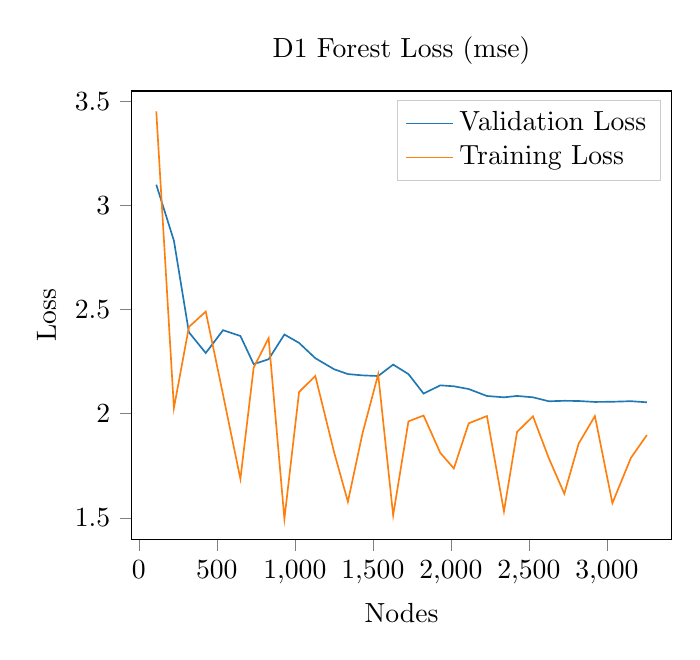
\begin{tikzpicture}

\definecolor{color0}{rgb}{0.12156862745098,0.466666666666667,0.705882352941177}
\definecolor{color1}{rgb}{1,0.498039215686275,0.0549019607843137}

\begin{axis}[
title={D1 Forest Loss (mse)},
xlabel={Nodes},
ylabel={Loss},
xmin=-45.2, xmax=3413.2,
ymin=1.39716473372065, ymax=3.54959287137901,
tick align=outside,
tick pos=left,
x grid style={white!69.01960784313725!black},
y grid style={white!69.01960784313725!black},
legend style={draw=white!80.0!black},
legend entries={{Validation Loss},{Training Loss}},
legend cell align={left}
]
\addlegendimage{no markers, color0}
\addlegendimage{no markers, color1}
\addplot [semithick, color0]
table {%
112 3.099414
225 2.83067283333333
321 2.39102644444444
429 2.29139341666666
540 2.40109925333333
651 2.37339475925926
736 2.23796610884354
832 2.26159860416667
933 2.38018869135802
1027 2.33997216
1131 2.26648565289256
1252 2.21328799074074
1340 2.19023631558185
1433 2.18411544217687
1534 2.18090040888889
1630 2.23576472135417
1728 2.19014305882353
1825 2.09658697530864
1932 2.13618122437673
2019 2.13164489166667
2114 2.11846286016629
2231 2.08506954545454
2340 2.07868846880907
2424 2.08525234722222
2526 2.07870938133334
2627 2.0597403382643
2727 2.06189921902149
2819 2.06102026020408
2923 2.05645187078874
3035 2.05740990666667
3154 2.06004291640652
3256 2.05470395572917
};
\addplot [semithick, color1]
table {%
112 3.45175522875817
225 2.02733741830065
321 2.41624382716049
429 2.49042199754902
540 2.09046266666667
651 1.68696614015977
736 2.22094349739896
832 2.36306469056372
933 1.49500237634148
1027 2.1041017124183
1131 2.18124516555934
1252 1.8136222290305
1340 1.57735496190587
1433 1.9039308206616
1534 2.18887645751634
1630 1.51230433261846
1728 1.96313598728996
1825 1.99136747155652
1932 1.81195049608024
2019 1.73705436111111
2114 1.95361812799194
2231 1.98871866526225
2340 1.53107354670917
2424 1.91228783133624
2526 1.98763636705882
2627 1.78730554298643
2727 1.61609948985538
2819 1.85681363211951
2923 1.98854853193755
3035 1.5705901503268
3154 1.78831822618052
3256 1.89748037300858
};
\end{axis}

\end{tikzpicture}
% This file was created by matplotlib2tikz v0.6.17.
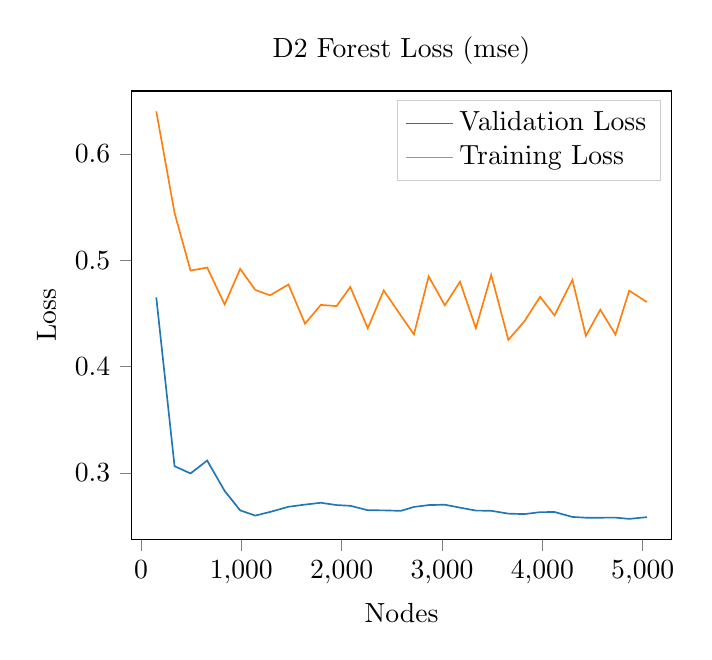
\begin{tikzpicture}

\definecolor{color0}{rgb}{0.12156862745098,0.466666666666667,0.705882352941177}
\definecolor{color1}{rgb}{1,0.498039215686275,0.0549019607843137}

\begin{axis}[
title={D2 Forest Loss (mse)},
xlabel={Nodes},
ylabel={Loss},
xmin=-91.4, xmax=5285.4,
ymin=0.237536420395422, ymax=0.659164932362123,
tick align=outside,
tick pos=left,
x grid style={white!69.01960784313725!black},
y grid style={white!69.01960784313725!black},
legend cell align={left},
legend entries={{Validation Loss},{Training Loss}},
legend style={draw=white!80.0!black}
]
\addlegendimage{no markers, color0}
\addlegendimage{no markers, color1}
\addplot [semithick, color0]
table {%
153 0.465
335 0.30625
494 0.299444444444445
660 0.3115625
834 0.283
989 0.264722222222223
1139 0.259795918367347
1286 0.263203125
1470 0.268086419753087
1635 0.27015
1792 0.271859504132232
1950 0.2696875
2086 0.269023668639053
2260 0.26484693877551
2419 0.264711111111111
2589 0.2642578125
2720 0.267923875432526
2867 0.269691358024692
3028 0.270013850415513
3179 0.2673
3337 0.264512471655329
3490 0.264318181818182
3661 0.261625708884688
3822 0.261206597222222
3977 0.26304
4121 0.263165680473372
4299 0.258539094650206
4433 0.25781887755102
4577 0.257829964328181
4728 0.257894444444444
4865 0.256701352757544
5041 0.258330078125
};
\addplot [semithick, color1]
table {%
153 0.64
335 0.5445
494 0.490222222222221
660 0.4930625
834 0.458360000000002
989 0.491805555555555
1139 0.472102040816325
1286 0.4669375
1470 0.477135802469137
1635 0.44025
1792 0.45794214876033
1950 0.456805555555556
2086 0.474828402366866
2260 0.435918367346937
2419 0.471586666666668
2589 0.447984375
2720 0.430204152249137
2867 0.484719135802468
3028 0.457531855955679
3179 0.479705
3337 0.436056689342402
3490 0.486134297520662
3661 0.425090737240075
3822 0.442678819444443
3977 0.465544
4121 0.448076923076924
4299 0.481530864197532
4433 0.428867346938776
4577 0.453453032104638
4728 0.430060000000001
4865 0.471308012486992
5041 0.46061328125
};
\end{axis}

\end{tikzpicture}

\section{Timings}
The following approximate timings were observed for each operation, taking into account errors due to CPU and memory caching by averaging:
\begin{itemize}
	\item Training - Dataset 1 - MSE - \textbf{0.45s}
	\item Training - Dataset 1 - MAE - \textbf{0.43s}
	\item Training - Dataset 2 - MSE - \textbf{19.95s}
	\item Training - Dataset 2 - MAE - \textbf{18.82s}
	\item Inference - Dataset 1 - \textbf{0.001s} (8$\mu$s per sample)
	\item Inference - Dataset 2 - \textbf{0.004s} (10$\mu$s per sample)
\end{itemize}
Notes:
\begin{enumerate}
	\item All timings were calculated using CPU nano-timing
	\item Training includes pruning
	\item All timings were calculated with the non-verbose mode
\end{enumerate}

\section{Conclusion}
We may conclude that using a decision tree may produce significant and acceptable results on certain types of datasets, with improvements on using random forests. The loss function does not have significant bearing on the results, since it gives contradicting results for two datasets.\\
The only references used for this Assignment were class notes, StackOverflow and python documentation.

\end{document}